% Options for packages loaded elsewhere
\PassOptionsToPackage{unicode}{hyperref}
\PassOptionsToPackage{hyphens}{url}
%
\documentclass[
]{book}
\usepackage{lmodern}
\usepackage{amssymb,amsmath}
\usepackage{ifxetex,ifluatex}
\ifnum 0\ifxetex 1\fi\ifluatex 1\fi=0 % if pdftex
  \usepackage[T1]{fontenc}
  \usepackage[utf8]{inputenc}
  \usepackage{textcomp} % provide euro and other symbols
\else % if luatex or xetex
  \usepackage{unicode-math}
  \defaultfontfeatures{Scale=MatchLowercase}
  \defaultfontfeatures[\rmfamily]{Ligatures=TeX,Scale=1}
\fi
% Use upquote if available, for straight quotes in verbatim environments
\IfFileExists{upquote.sty}{\usepackage{upquote}}{}
\IfFileExists{microtype.sty}{% use microtype if available
  \usepackage[]{microtype}
  \UseMicrotypeSet[protrusion]{basicmath} % disable protrusion for tt fonts
}{}
\makeatletter
\@ifundefined{KOMAClassName}{% if non-KOMA class
  \IfFileExists{parskip.sty}{%
    \usepackage{parskip}
  }{% else
    \setlength{\parindent}{0pt}
    \setlength{\parskip}{6pt plus 2pt minus 1pt}}
}{% if KOMA class
  \KOMAoptions{parskip=half}}
\makeatother
\usepackage{xcolor}
\IfFileExists{xurl.sty}{\usepackage{xurl}}{} % add URL line breaks if available
\IfFileExists{bookmark.sty}{\usepackage{bookmark}}{\usepackage{hyperref}}
\hypersetup{
  pdftitle={Rat DCIS study},
  pdfauthor={Anne Trinh},
  hidelinks,
  pdfcreator={LaTeX via pandoc}}
\urlstyle{same} % disable monospaced font for URLs
\usepackage{color}
\usepackage{fancyvrb}
\newcommand{\VerbBar}{|}
\newcommand{\VERB}{\Verb[commandchars=\\\{\}]}
\DefineVerbatimEnvironment{Highlighting}{Verbatim}{commandchars=\\\{\}}
% Add ',fontsize=\small' for more characters per line
\usepackage{framed}
\definecolor{shadecolor}{RGB}{248,248,248}
\newenvironment{Shaded}{\begin{snugshade}}{\end{snugshade}}
\newcommand{\AlertTok}[1]{\textcolor[rgb]{0.94,0.16,0.16}{#1}}
\newcommand{\AnnotationTok}[1]{\textcolor[rgb]{0.56,0.35,0.01}{\textbf{\textit{#1}}}}
\newcommand{\AttributeTok}[1]{\textcolor[rgb]{0.77,0.63,0.00}{#1}}
\newcommand{\BaseNTok}[1]{\textcolor[rgb]{0.00,0.00,0.81}{#1}}
\newcommand{\BuiltInTok}[1]{#1}
\newcommand{\CharTok}[1]{\textcolor[rgb]{0.31,0.60,0.02}{#1}}
\newcommand{\CommentTok}[1]{\textcolor[rgb]{0.56,0.35,0.01}{\textit{#1}}}
\newcommand{\CommentVarTok}[1]{\textcolor[rgb]{0.56,0.35,0.01}{\textbf{\textit{#1}}}}
\newcommand{\ConstantTok}[1]{\textcolor[rgb]{0.00,0.00,0.00}{#1}}
\newcommand{\ControlFlowTok}[1]{\textcolor[rgb]{0.13,0.29,0.53}{\textbf{#1}}}
\newcommand{\DataTypeTok}[1]{\textcolor[rgb]{0.13,0.29,0.53}{#1}}
\newcommand{\DecValTok}[1]{\textcolor[rgb]{0.00,0.00,0.81}{#1}}
\newcommand{\DocumentationTok}[1]{\textcolor[rgb]{0.56,0.35,0.01}{\textbf{\textit{#1}}}}
\newcommand{\ErrorTok}[1]{\textcolor[rgb]{0.64,0.00,0.00}{\textbf{#1}}}
\newcommand{\ExtensionTok}[1]{#1}
\newcommand{\FloatTok}[1]{\textcolor[rgb]{0.00,0.00,0.81}{#1}}
\newcommand{\FunctionTok}[1]{\textcolor[rgb]{0.00,0.00,0.00}{#1}}
\newcommand{\ImportTok}[1]{#1}
\newcommand{\InformationTok}[1]{\textcolor[rgb]{0.56,0.35,0.01}{\textbf{\textit{#1}}}}
\newcommand{\KeywordTok}[1]{\textcolor[rgb]{0.13,0.29,0.53}{\textbf{#1}}}
\newcommand{\NormalTok}[1]{#1}
\newcommand{\OperatorTok}[1]{\textcolor[rgb]{0.81,0.36,0.00}{\textbf{#1}}}
\newcommand{\OtherTok}[1]{\textcolor[rgb]{0.56,0.35,0.01}{#1}}
\newcommand{\PreprocessorTok}[1]{\textcolor[rgb]{0.56,0.35,0.01}{\textit{#1}}}
\newcommand{\RegionMarkerTok}[1]{#1}
\newcommand{\SpecialCharTok}[1]{\textcolor[rgb]{0.00,0.00,0.00}{#1}}
\newcommand{\SpecialStringTok}[1]{\textcolor[rgb]{0.31,0.60,0.02}{#1}}
\newcommand{\StringTok}[1]{\textcolor[rgb]{0.31,0.60,0.02}{#1}}
\newcommand{\VariableTok}[1]{\textcolor[rgb]{0.00,0.00,0.00}{#1}}
\newcommand{\VerbatimStringTok}[1]{\textcolor[rgb]{0.31,0.60,0.02}{#1}}
\newcommand{\WarningTok}[1]{\textcolor[rgb]{0.56,0.35,0.01}{\textbf{\textit{#1}}}}
\usepackage{longtable,booktabs}
% Correct order of tables after \paragraph or \subparagraph
\usepackage{etoolbox}
\makeatletter
\patchcmd\longtable{\par}{\if@noskipsec\mbox{}\fi\par}{}{}
\makeatother
% Allow footnotes in longtable head/foot
\IfFileExists{footnotehyper.sty}{\usepackage{footnotehyper}}{\usepackage{footnote}}
\makesavenoteenv{longtable}
\usepackage{graphicx,grffile}
\makeatletter
\def\maxwidth{\ifdim\Gin@nat@width>\linewidth\linewidth\else\Gin@nat@width\fi}
\def\maxheight{\ifdim\Gin@nat@height>\textheight\textheight\else\Gin@nat@height\fi}
\makeatother
% Scale images if necessary, so that they will not overflow the page
% margins by default, and it is still possible to overwrite the defaults
% using explicit options in \includegraphics[width, height, ...]{}
\setkeys{Gin}{width=\maxwidth,height=\maxheight,keepaspectratio}
% Set default figure placement to htbp
\makeatletter
\def\fps@figure{htbp}
\makeatother
\setlength{\emergencystretch}{3em} % prevent overfull lines
\providecommand{\tightlist}{%
  \setlength{\itemsep}{0pt}\setlength{\parskip}{0pt}}
\setcounter{secnumdepth}{5}
\usepackage{booktabs}
\usepackage{booktabs}
\usepackage{longtable}
\usepackage{array}
\usepackage{multirow}
\usepackage{wrapfig}
\usepackage{float}
\usepackage{colortbl}
\usepackage{pdflscape}
\usepackage{tabu}
\usepackage{threeparttable}
\usepackage{threeparttablex}
\usepackage[normalem]{ulem}
\usepackage{makecell}
\usepackage[]{natbib}
\bibliographystyle{apalike}

\title{Rat DCIS study}
\author{Anne Trinh}
\date{2020-11-07}

\begin{document}
\maketitle

{
\setcounter{tocdepth}{1}
\tableofcontents
}
This is a summary of the code required in the study: `insert study name'

\hypertarget{prerequisites}{%
\chapter{Prerequisites}\label{prerequisites}}

\hypertarget{packages-and-software}{%
\section{Packages and Software}\label{packages-and-software}}

The following packages are required to conduct the analyses described below.

In house scripts are deposited in the rscript folder.

\begin{Shaded}
\begin{Highlighting}[]
\KeywordTok{library}\NormalTok{(AnnotationHub)}
\KeywordTok{library}\NormalTok{(biomaRt)}
\KeywordTok{library}\NormalTok{(Biostrings)}
\KeywordTok{library}\NormalTok{(colorspace)}
\KeywordTok{library}\NormalTok{(DESeq2)}
\KeywordTok{library}\NormalTok{(dplyr)}
\KeywordTok{library}\NormalTok{(DT)}
\KeywordTok{library}\NormalTok{(ensembldb)}
\KeywordTok{library}\NormalTok{(EnsDb.Hsapiens.v86)}
\KeywordTok{library}\NormalTok{(GenVisR)}
\KeywordTok{library}\NormalTok{(GenomicFeatures)}
\KeywordTok{library}\NormalTok{(ggplot2)}
\KeywordTok{library}\NormalTok{(gplots)}
\KeywordTok{library}\NormalTok{(GSEABase)}
\KeywordTok{library}\NormalTok{(GSVA)}
\KeywordTok{library}\NormalTok{(heatmap.plus)}
\KeywordTok{library}\NormalTok{(HTSanalyzeR2)}
\CommentTok{#library(kableExtra)}
\KeywordTok{library}\NormalTok{(limma)}
\KeywordTok{library}\NormalTok{(matrixStats)}
\KeywordTok{library}\NormalTok{(pamr)}
\KeywordTok{library}\NormalTok{(reshape2)}
\KeywordTok{library}\NormalTok{(RColorBrewer)}
\KeywordTok{library}\NormalTok{(scales)}
\KeywordTok{library}\NormalTok{(spatstat)}
\KeywordTok{library}\NormalTok{(tcR)}
\KeywordTok{library}\NormalTok{(vcfR)}
\KeywordTok{library}\NormalTok{(xlsx)}
\KeywordTok{library}\NormalTok{(writexl)}

\NormalTok{DiffCols=}\KeywordTok{hue_pal}\NormalTok{()(}\DecValTok{8}\NormalTok{)}
\KeywordTok{palette}\NormalTok{(}\KeywordTok{brewer.pal}\NormalTok{(}\DecValTok{9}\NormalTok{, }\StringTok{"Set1"}\NormalTok{))}
\NormalTok{RdBu=}\KeywordTok{brewer.pal}\NormalTok{(}\DecValTok{11}\NormalTok{, }\StringTok{"RdBu"}\NormalTok{)}
\NormalTok{SetCols=}\KeywordTok{brewer.pal}\NormalTok{(}\DecValTok{12}\NormalTok{, }\StringTok{"Set3"}\NormalTok{)}

\KeywordTok{source}\NormalTok{(}\StringTok{"../rscript/cnFreq_fn.R"}\NormalTok{) }\CommentTok{#modified version of GenVisR}
\KeywordTok{source}\NormalTok{(}\StringTok{"../rscript/merge_contig.R"}\NormalTok{)}
\KeywordTok{source}\NormalTok{(}\StringTok{"../rscript/gseaCode.R"}\NormalTok{)}
\KeywordTok{source}\NormalTok{(}\StringTok{"../rscript/ContingencyTable.R"}\NormalTok{)}
\KeywordTok{source}\NormalTok{(}\StringTok{"../rscript/PvalueHeatMap.R"}\NormalTok{)}
\KeywordTok{source}\NormalTok{(}\StringTok{"../rscript/BootstrapShannonIdx.R"}\NormalTok{)}
\KeywordTok{source}\NormalTok{(}\StringTok{"../rscript/CreateRnor87db.R"}\NormalTok{)}
\KeywordTok{source}\NormalTok{(}\StringTok{"../rscript/FindRatAAHomolog.R"}\NormalTok{)}

\NormalTok{firstup <-}\StringTok{ }\ControlFlowTok{function}\NormalTok{(x) \{}
  \KeywordTok{substr}\NormalTok{(x, }\DecValTok{1}\NormalTok{, }\DecValTok{1}\NormalTok{) <-}\StringTok{ }\KeywordTok{toupper}\NormalTok{(}\KeywordTok{substr}\NormalTok{(x, }\DecValTok{1}\NormalTok{, }\DecValTok{1}\NormalTok{))}
\NormalTok{  x}
\NormalTok{\}}

\NormalTok{ColMerge=}\KeywordTok{matrix}\NormalTok{(}\KeywordTok{c}\NormalTok{(}\StringTok{"#FFC82F"}\NormalTok{, }\StringTok{"#FFEDBC"}\NormalTok{, }\StringTok{"#73FDFE"}\NormalTok{,}\StringTok{"#D2FFFF"}\NormalTok{, }\StringTok{"#FF41FF"}\NormalTok{, }\StringTok{"#FECAFF"}\NormalTok{, }\StringTok{"#5D5D5D"}\NormalTok{, }\StringTok{"#BEBEBE"}\NormalTok{), }\DataTypeTok{ncol=}\DecValTok{2}\NormalTok{, }\DataTypeTok{byrow =}\NormalTok{ T)}
\KeywordTok{rownames}\NormalTok{(ColMerge)=}\KeywordTok{c}\NormalTok{(}\StringTok{"LY"}\NormalTok{,}\StringTok{"PDL1"}\NormalTok{, }\StringTok{"PDL1+LY"}\NormalTok{,}\StringTok{"Vehicle"}\NormalTok{)}

\NormalTok{Hsedb<-EnsDb.Hsapiens.v86}
\end{Highlighting}
\end{Shaded}

\hypertarget{external-software}{%
\section{External software}\label{external-software}}

The following external software was utilised:

\begin{longtable}[]{@{}ll@{}}
\toprule
\begin{minipage}[b]{0.10\columnwidth}\raggedright
Software\strut
\end{minipage} & \begin{minipage}[b]{0.85\columnwidth}\raggedright
Function\strut
\end{minipage}\tabularnewline
\midrule
\endhead
\begin{minipage}[t]{0.10\columnwidth}\raggedright
\href{http://bio-bwa.sourceforge.net/}{bwa}\strut
\end{minipage} & \begin{minipage}[t]{0.85\columnwidth}\raggedright
Alignment of WGS data to reference\strut
\end{minipage}\tabularnewline
\begin{minipage}[t]{0.10\columnwidth}\raggedright
\href{https://software.broadinstitute.org/gatk/}{GATK4}\strut
\end{minipage} & \begin{minipage}[t]{0.85\columnwidth}\raggedright
Mutation calling, done by NYGC. Mutation calling from RNA (Haplotype caller)\strut
\end{minipage}\tabularnewline
\begin{minipage}[t]{0.10\columnwidth}\raggedright
\href{https://github.com/Illumina/strelka}{strelka}\strut
\end{minipage} & \begin{minipage}[t]{0.85\columnwidth}\raggedright
Mutation calling, done by NYGC\strut
\end{minipage}\tabularnewline
\begin{minipage}[t]{0.10\columnwidth}\raggedright
\href{http://compbio.med.harvard.edu/BIC-seq/}{BICseq}\strut
\end{minipage} & \begin{minipage}[t]{0.85\columnwidth}\raggedright
CNV calling\strut
\end{minipage}\tabularnewline
\begin{minipage}[t]{0.10\columnwidth}\raggedright
\href{https://sourceforge.net/projects/gemlibrary/files/gem-library/}{GEM3}\strut
\end{minipage} & \begin{minipage}[t]{0.85\columnwidth}\raggedright
create mappability files for CNV calling\strut
\end{minipage}\tabularnewline
\begin{minipage}[t]{0.10\columnwidth}\raggedright
\href{https://github.com/alexdobin/STAR}{STAR}\strut
\end{minipage} & \begin{minipage}[t]{0.85\columnwidth}\raggedright
Alignment of RNAseq data\strut
\end{minipage}\tabularnewline
\begin{minipage}[t]{0.10\columnwidth}\raggedright
\href{https://github.com/deweylab/RSEM}{RSEM}\strut
\end{minipage} & \begin{minipage}[t]{0.85\columnwidth}\raggedright
Calculate RSEM, TPM, FPKM from RNAseq data\strut
\end{minipage}\tabularnewline
\begin{minipage}[t]{0.10\columnwidth}\raggedright
\href{https://github.com/liulab-dfci/TRUST4}{TRUST4}\strut
\end{minipage} & \begin{minipage}[t]{0.85\columnwidth}\raggedright
assignment of T and B cell clonotypes from RNA-seq data\strut
\end{minipage}\tabularnewline
\begin{minipage}[t]{0.10\columnwidth}\raggedright
\href{https://gatkforums.broadinstitute.org/gatk/discussion/4154/howto-install-and-run-oncotator-for-the-first-time}{Oncotator}\strut
\end{minipage} & \begin{minipage}[t]{0.85\columnwidth}\raggedright
Annotation of genetic variants\strut
\end{minipage}\tabularnewline
\begin{minipage}[t]{0.10\columnwidth}\raggedright
\href{https://qupath.github.io/}{QuPath}\strut
\end{minipage} & \begin{minipage}[t]{0.85\columnwidth}\raggedright
Tool for cell segmentation and extraction of features from IF images\strut
\end{minipage}\tabularnewline
\begin{minipage}[t]{0.10\columnwidth}\raggedright
\href{http://www.htslib.org/}{samtools, bcftools}\strut
\end{minipage} & \begin{minipage}[t]{0.85\columnwidth}\raggedright
querying and dispalying information from bam files, extracting allelic depth at specific genomic locations\strut
\end{minipage}\tabularnewline
\begin{minipage}[t]{0.10\columnwidth}\raggedright
\href{https://cibersort.stanford.edu/}{CIBERSORT}\strut
\end{minipage} & \begin{minipage}[t]{0.85\columnwidth}\raggedright
inferring immune composition from RNA\strut
\end{minipage}\tabularnewline
\begin{minipage}[t]{0.10\columnwidth}\raggedright
\href{https://github.com/arq5x/lumpy-sv}{lumpy}\strut
\end{minipage} & \begin{minipage}[t]{0.85\columnwidth}\raggedright
structural variants\strut
\end{minipage}\tabularnewline
\begin{minipage}[t]{0.10\columnwidth}\raggedright
\href{https://genome.unc.edu/pubsup/breastGEO/PAM50.zip}{PAM50}\strut
\end{minipage} & \begin{minipage}[t]{0.85\columnwidth}\raggedright
code from parker et al 2009 to infer PAM50 subtypes\strut
\end{minipage}\tabularnewline
\bottomrule
\end{longtable}

\hypertarget{annotations}{%
\section{Annotations}\label{annotations}}

\hypertarget{genomic-properties}{%
\subsection{Genomic properties}\label{genomic-properties}}

Information on chromosome sizes, cytobands and centromere locations were obtained from the \href{http://hgdownload.soe.ucsc.edu/goldenPath/rn6/database/}{UCSC genome browser}.

The following annotation data for the hg19/b37/GRCh37 genome is required:

\begin{longtable}[]{@{}ll@{}}
\toprule
\begin{minipage}[b]{0.30\columnwidth}\raggedright
Data Type\strut
\end{minipage} & \begin{minipage}[b]{0.64\columnwidth}\raggedright
Download link\strut
\end{minipage}\tabularnewline
\midrule
\endhead
\begin{minipage}[t]{0.30\columnwidth}\raggedright
ref. genome\strut
\end{minipage} & \begin{minipage}[t]{0.64\columnwidth}\raggedright
\url{http://hgdownload.soe.ucsc.edu/goldenPath/rn6/bigZips/rn6.fa.gz}\strut
\end{minipage}\tabularnewline
\begin{minipage}[t]{0.30\columnwidth}\raggedright
refSeq annot\strut
\end{minipage} & \begin{minipage}[t]{0.64\columnwidth}\raggedright
\url{http://hgdownload.soe.ucsc.edu/goldenPath/rn6/bigZips/genes/rn6.refGene.gtf.gz}\strut
\end{minipage}\tabularnewline
\begin{minipage}[t]{0.30\columnwidth}\raggedright
refSeq annot\strut
\end{minipage} & \begin{minipage}[t]{0.64\columnwidth}\raggedright
\url{http://hgdownload.soe.ucsc.edu/goldenPath/rn6/bigZips/genes/rn6.ncbiRefSeq.gtf.gz}\strut
\end{minipage}\tabularnewline
\begin{minipage}[t]{0.30\columnwidth}\raggedright
gff3 file\strut
\end{minipage} & \begin{minipage}[t]{0.64\columnwidth}\raggedright
for TRUST4 (\url{ftp://ftp.ensembl.org/pub/release-100/gff3/rattus_norvegicus/Rattus_norvegicus.Rnor_6.0.100.gff3.gz})\strut
\end{minipage}\tabularnewline
\begin{minipage}[t]{0.30\columnwidth}\raggedright
gene lengths\strut
\end{minipage} & \begin{minipage}[t]{0.64\columnwidth}\raggedright
Extracted from GRCh37.75.gtf file from \href{ftp://ftp.ensembl.org/pub/grch37/current/gtf/homo_sapiens/}{ensembl}\strut
\end{minipage}\tabularnewline
\begin{minipage}[t]{0.30\columnwidth}\raggedright
hg19cytoBand\strut
\end{minipage} & \begin{minipage}[t]{0.64\columnwidth}\raggedright
\href{http://hgdownload.cse.ucsc.edu/goldenPath/hg19/database/cytoBand.txt.gz}{ucsc server} of all cytoband locations\strut
\end{minipage}\tabularnewline
\begin{minipage}[t]{0.30\columnwidth}\raggedright
chromosome sizes\strut
\end{minipage} & \begin{minipage}[t]{0.64\columnwidth}\raggedright
\href{http://hgdownload.cse.ucsc.edu/goldenPath/hg19/database/chromInfo.txt.gz}{uscs genome browser}\strut
\end{minipage}\tabularnewline
\begin{minipage}[t]{0.30\columnwidth}\raggedright
\href{https://bioconductor.org/packages/release/bioc/html/biomaRt.html}{biomart}\strut
\end{minipage} & \begin{minipage}[t]{0.64\columnwidth}\raggedright
conversion between gene symbol, ensbl and entrez was faciliated using biomart package\strut
\end{minipage}\tabularnewline
\bottomrule
\end{longtable}

Below is the summary of chromosome sizes and centromere locations:

\begin{verbatim}
##   chrom chromStart chromEnd name gieStain
## 1  chr1          0 10704345  p13     gneg
## 2  chr1   10704345 25618263  p12     gvar
## 3  chr1   25618263 40652454  p11     gneg
## 4  chr1   40652454 51356799  q11     gpos
## 5  chr1   51356799 73607402  q12     gneg
## 6  chr1   73607402 95016091  q21     gpos
\end{verbatim}

Create a TxDb object from a gtf file and save information: {Not sure which version to use??}

Below is an example of the gene annotation files

\begin{verbatim}
## GRanges object with 6 ranges and 2 metadata columns:
##          seqnames          ranges strand |     gene_id gene_width
##             <Rle>       <IRanges>  <Rle> | <character>  <integer>
##   Vom2r3     chr1   396700-409676      + |      Vom2r3      12977
##    Lrp11     chr1 1702696-1731210      + |       Lrp11      28515
##    Nup43     chr1 1771721-1781554      + |       Nup43       9834
##    Lats1     chr1 1784078-1817310      + |       Lats1      33233
##   Katna1     chr1 1826170-1867786      + |      Katna1      41617
##    Ppil4     chr1 1897350-1930311      + |       Ppil4      32962
##   -------
##   seqinfo: 22 sequences from an unspecified genome; no seqlengths
\end{verbatim}

\hypertarget{gene-name-homologs-between-organisms}{%
\subsection{Gene name homologs between organisms}\label{gene-name-homologs-between-organisms}}

Biomart was used to convert between rat, mouse and human gene symbols and ensembl ids. Below is an example of the human gene names mapped to the rat homolog

{
Figure out what is required here for later analysis
}

\begin{verbatim}
##   HGNC.symbol RGD.symbol
## 1        TAB1       Tab1
## 2        PHF1       Phf1
## 3       RNF39      Rnf39
## 4      IGSF10     Igsf10
## 5     TMEM130    Tmem130
## 6       EFNB1      Efnb1
\end{verbatim}

\hypertarget{gene-signatures-and-data-bases}{%
\subsection{Gene signatures and data-bases}\label{gene-signatures-and-data-bases}}

Gene sets/signatures were obtained from the following sources:

\begin{longtable}[]{@{}ll@{}}
\toprule
\begin{minipage}[b]{0.21\columnwidth}\raggedright
Source\strut
\end{minipage} & \begin{minipage}[b]{0.73\columnwidth}\raggedright
Description\strut
\end{minipage}\tabularnewline
\midrule
\endhead
\begin{minipage}[t]{0.21\columnwidth}\raggedright
\href{https://www.iedb.org/}{IEDB}\strut
\end{minipage} & \begin{minipage}[t]{0.73\columnwidth}\raggedright
database of immune epitopes\strut
\end{minipage}\tabularnewline
\begin{minipage}[t]{0.21\columnwidth}\raggedright
\href{http://software.broadinstitute.org/gsea/msigdb/index.jsp}{MsigDB}\strut
\end{minipage} & \begin{minipage}[t]{0.73\columnwidth}\raggedright
c2, c5, hallmark set of curated pathway gene sets\strut
\end{minipage}\tabularnewline
\begin{minipage}[t]{0.21\columnwidth}\raggedright
\href{}{Metacore}\strut
\end{minipage} & \begin{minipage}[t]{0.73\columnwidth}\raggedright
Process Networks and Pathway Maps data bases\strut
\end{minipage}\tabularnewline
\begin{minipage}[t]{0.21\columnwidth}\raggedright
\href{https://cancer.sanger.ac.uk/census}{COSMIC}\strut
\end{minipage} & \begin{minipage}[t]{0.73\columnwidth}\raggedright
database of concensus oncogenes\strut
\end{minipage}\tabularnewline
\begin{minipage}[t]{0.21\columnwidth}\raggedright
\href{https://www.immport.org/home}{ImmPort}\strut
\end{minipage} & \begin{minipage}[t]{0.73\columnwidth}\raggedright
List of immune related genes\strut
\end{minipage}\tabularnewline
\begin{minipage}[t]{0.21\columnwidth}\raggedright
\href{https://www.innatedb.com/}{InnateDB}\strut
\end{minipage} & \begin{minipage}[t]{0.73\columnwidth}\raggedright
List of genes associated with innate immune system\strut
\end{minipage}\tabularnewline
\begin{minipage}[t]{0.21\columnwidth}\raggedright
\href{https://dx.doi.org/10.1038/s41586-019-1032-7}{Rosenthal 2019}\strut
\end{minipage} & \begin{minipage}[t]{0.73\columnwidth}\raggedright
genes associated with MHC-I presentation\strut
\end{minipage}\tabularnewline
\begin{minipage}[t]{0.21\columnwidth}\raggedright
\href{http://dx.doi.org/10.1016/j.immuni.2018.03.023}{Thorsson 2018}\strut
\end{minipage} & \begin{minipage}[t]{0.73\columnwidth}\raggedright
Immune gene signatures curated from studies by Wolf, Calabro, Teschendorff, Beck, Chang\strut
\end{minipage}\tabularnewline
\begin{minipage}[t]{0.21\columnwidth}\raggedright
\href{https://www.ncbi.nlm.nih.gov/pubmed/22437870}{Pardoll}, \href{https://www.ncbi.nlm.nih.gov/pubmed/28990586}{Wykes}\strut
\end{minipage} & \begin{minipage}[t]{0.73\columnwidth}\raggedright
Immune checkpoint genes\strut
\end{minipage}\tabularnewline
\begin{minipage}[t]{0.21\columnwidth}\raggedright
\href{https://cancerdiscovery.aacrjournals.org/content/early/2017/09/19/2159-8290.CD-17-0222}{gil del alcazar 2017}\strut
\end{minipage} & \begin{minipage}[t]{0.73\columnwidth}\raggedright
Supplementary table 5: list of activation, dysfunction gene signatures\strut
\end{minipage}\tabularnewline
\begin{minipage}[t]{0.21\columnwidth}\raggedright
\href{https://www.ncbi.nlm.nih.gov/pmc/articles/PMC6029450/}{Bailey 2018}\strut
\end{minipage} & \begin{minipage}[t]{0.73\columnwidth}\raggedright
List of 10 most comon tumor pathways\strut
\end{minipage}\tabularnewline
\begin{minipage}[t]{0.21\columnwidth}\raggedright
\href{https://pubmed.ncbi.nlm.nih.gov/29247016/}{Chang 2018}\strut
\end{minipage} & \begin{minipage}[t]{0.73\columnwidth}\raggedright
Common mutation locations in cancer\strut
\end{minipage}\tabularnewline
\bottomrule
\end{longtable}

The PAM50 signature was implemented using the scripts provided in supplementary from \href{https://genome.unc.edu/pubsup/breastGEO/PAM50.zip}{Parker et al 2010}. These gene lists can be found in the annotations folder

\hypertarget{human-gene-homologs}{%
\subsubsection{Human gene homologs}\label{human-gene-homologs}}

Below, lists of common mutations in cancer are loaded and the ``homolog'' in rat is determined using an in-house script. The steps involved are:

\begin{itemize}
\tightlist
\item
  determine the amino acid context in human (find 5 a.a. prior and after)
\item
  find the region with most amino acid homology in rat (2 or less differences)
\item
  check whether the amino acid of interest is present in rat
\end{itemize}

An example of the output is shown

\begin{verbatim}
##   Gene AAno AA1 Variant RatGene    Sequence         HumProt            RatProt
## 1 NRAS   61   Q       R    Nras LDTAGQEEYSA ENSP00000358548 ENSRNOP00000036381
## 2 NRAS   61   Q       K    Nras LDTAGQEEYSA ENSP00000358548 ENSRNOP00000036381
## 3 NRAS   61   Q       L    Nras LDTAGQEEYSA ENSP00000358548 ENSRNOP00000036381
## 4 NRAS   61   Q       H    Nras LDTAGQEEYSA ENSP00000358548 ENSRNOP00000036381
## 5 NRAS   61   Q       P    Nras LDTAGQEEYSA ENSP00000358548 ENSRNOP00000036381
## 6 NRAS   61   Q       *    Nras LDTAGQEEYSA ENSP00000358548 ENSRNOP00000036381
##   RatAAno RatSequence
## 1      61 LDTAGQEEYSA
## 2      61 LDTAGQEEYSA
## 3      61 LDTAGQEEYSA
## 4      61 LDTAGQEEYSA
## 5      61 LDTAGQEEYSA
## 6      61 LDTAGQEEYSA
\end{verbatim}

\hypertarget{gsea-compendiums}{%
\subsubsection{GSEA compendiums}\label{gsea-compendiums}}

For pathway analysis, the c2 (pathway), Hallmark and c5 (Gene Ontology). In addition, metacore pathways (pathway maps and process networks) were obtained and loaded below. This gives a list of 7 different data-sets to interrogate
{
CHECK: When GSVA is run, which input is required??
}

\hypertarget{intro}{%
\chapter{Cohort summary}\label{intro}}

Below we assess summary statistics on clinico-pathological features of this data set. This includes information on:

\begin{itemize}
\tightlist
\item
  treatment
\item
  tumor size
\item
  growth rates (mm/week)
\item
  number of tumors per rat
\end{itemize}

\hypertarget{calculating-growth-rates}{%
\section{Calculating growth rates}\label{calculating-growth-rates}}

In this section, we estimate the growth rates of the samples: Below is a plot of the tumor size per week for each recorded tumor, color-coded according to treatment. Time is measured at the first time point at which a tumor is palpated. Spontaneous large tumors are assumed to have a tumor size of 0 or 1 one week prior to palpating.

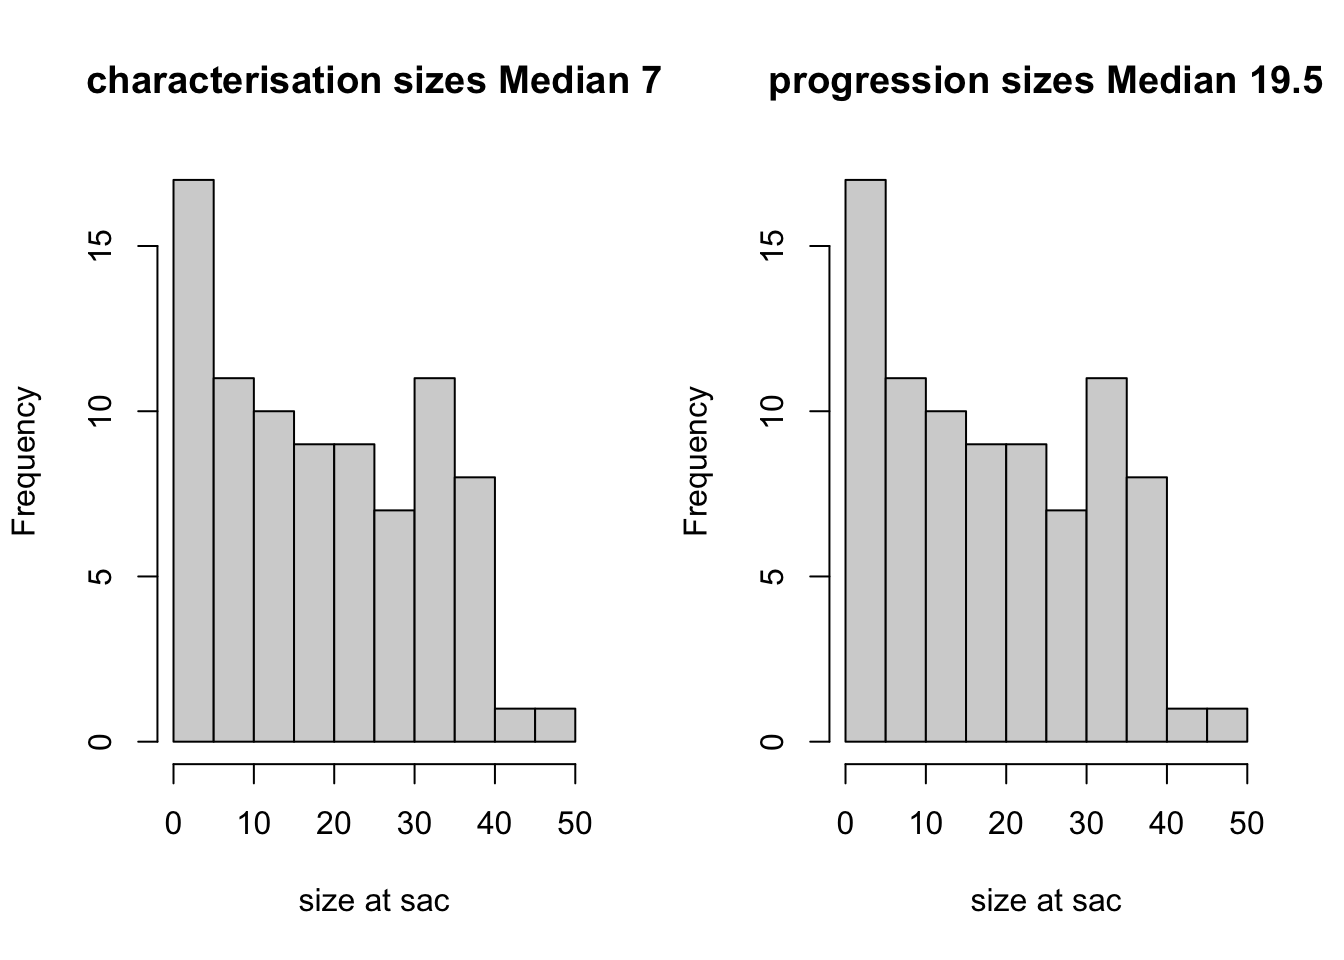
\includegraphics{RatDCIS-bookdown_files/figure-latex/unnamed-chunk-10-1.pdf} 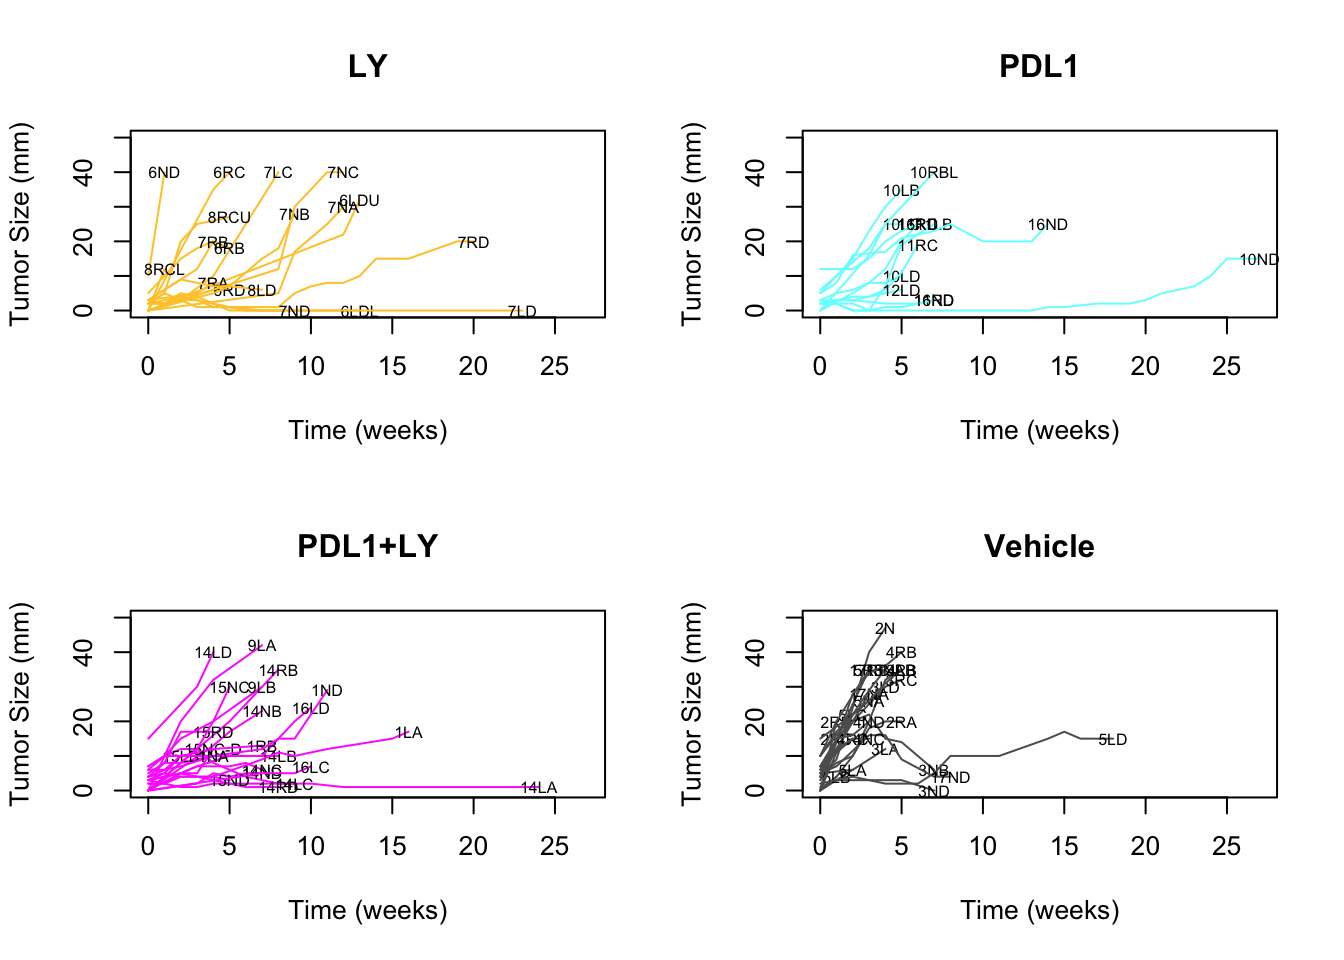
\includegraphics{RatDCIS-bookdown_files/figure-latex/unnamed-chunk-10-2.pdf}

These tumors doesn't have growth rate data: 17N\_B.

We can then compute the growth rate for the above samples by considering the change in size over a given period of time using a linear regression model. Below is the histogram of growth rates:

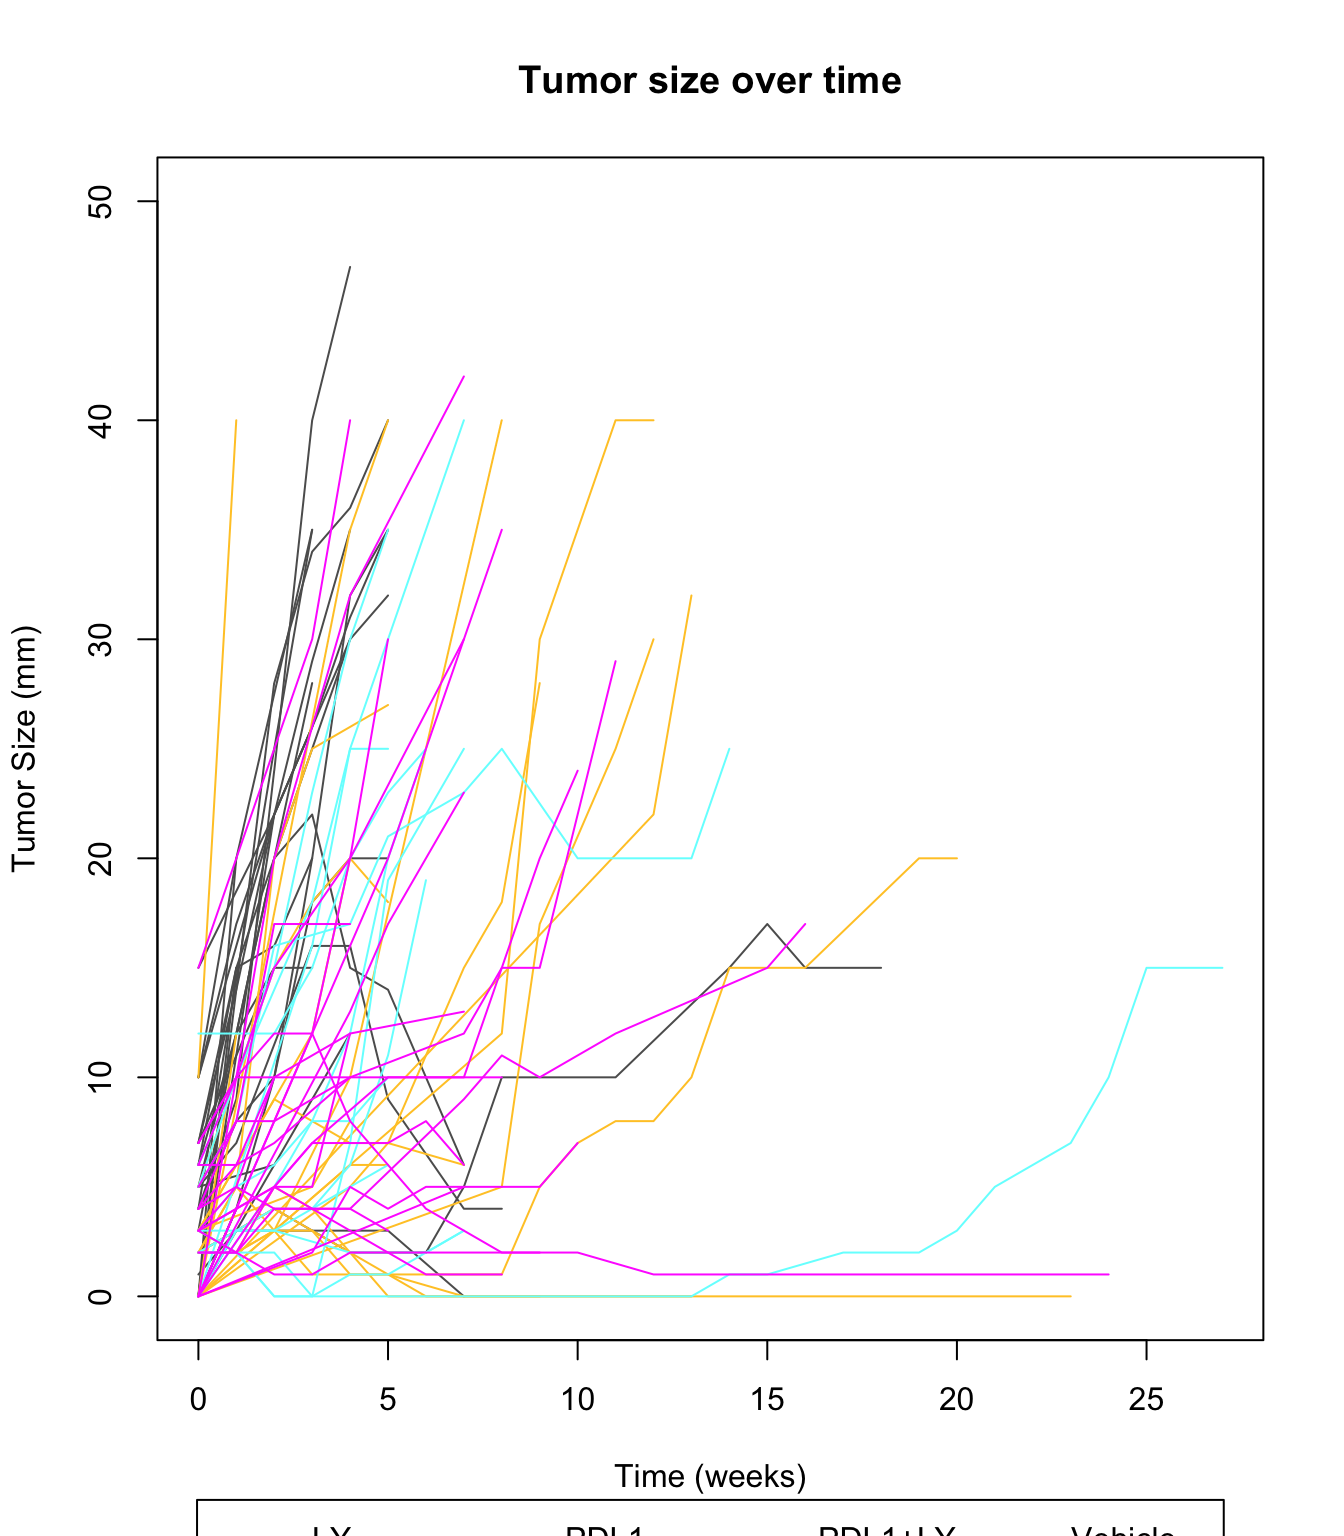
\includegraphics{RatDCIS-bookdown_files/figure-latex/unnamed-chunk-11-1.pdf}

Based on the above distribution, a cut-off of 2mm/week may be an optimal cut-off to separate growing and stable tumors. Below are growth rates of tumors under different treatments:

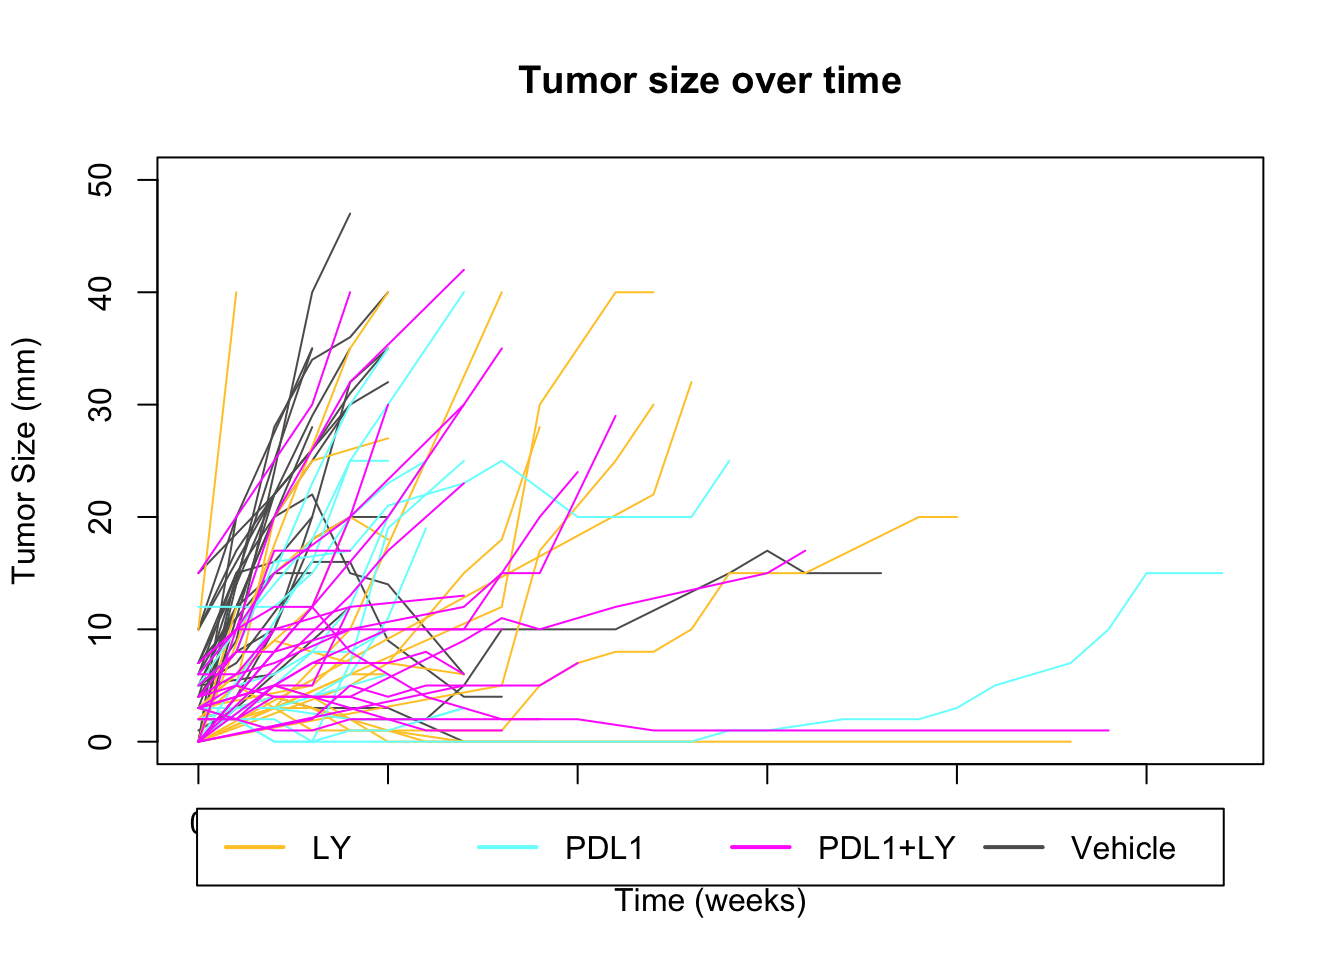
\includegraphics{RatDCIS-bookdown_files/figure-latex/unnamed-chunk-12-1.pdf}

We can calculate the p.values below, using a t.test. The growth rates comparing the treatment to the controls are:

\begin{verbatim}
## [1] "LY samples"
\end{verbatim}

\begin{verbatim}
## 
##  Wilcoxon rank sum test with continuity correction
## 
## data:  d1$growthrate[d1$treatment == "LY"] and d1$growthrate[d1$treatment == "Vehicle"]
## W = 165.5, p-value = 0.1718
## alternative hypothesis: true location shift is not equal to 0
\end{verbatim}

\begin{verbatim}
## [1] "PDL1 samples"
\end{verbatim}

\begin{verbatim}
## 
##  Wilcoxon rank sum test with continuity correction
## 
## data:  d1$growthrate[d1$treatment == "PDL1"] and d1$growthrate[d1$treatment == "Vehicle"]
## W = 103, p-value = 0.051
## alternative hypothesis: true location shift is not equal to 0
\end{verbatim}

\begin{verbatim}
## [1] "PDL1+LY samples"
\end{verbatim}

\begin{verbatim}
## 
##  Wilcoxon rank sum test with continuity correction
## 
## data:  d1$growthrate[d1$treatment == "PDL1+LY"] and d1$growthrate[d1$treatment == "Vehicle"]
## W = 154.5, p-value = 0.006713
## alternative hypothesis: true location shift is not equal to 0
\end{verbatim}

This shows a smaller growth-rate in PDL1 single and double treated cases compared to the vehicles.

Overall the distribution of growing vs stable tumors is shown below:

\begin{verbatim}
## 
##   grow stable 
##     47     31
\end{verbatim}

We can replot the previous graphs according to growth, and color code according to whether it is a fast or slow growing tumor

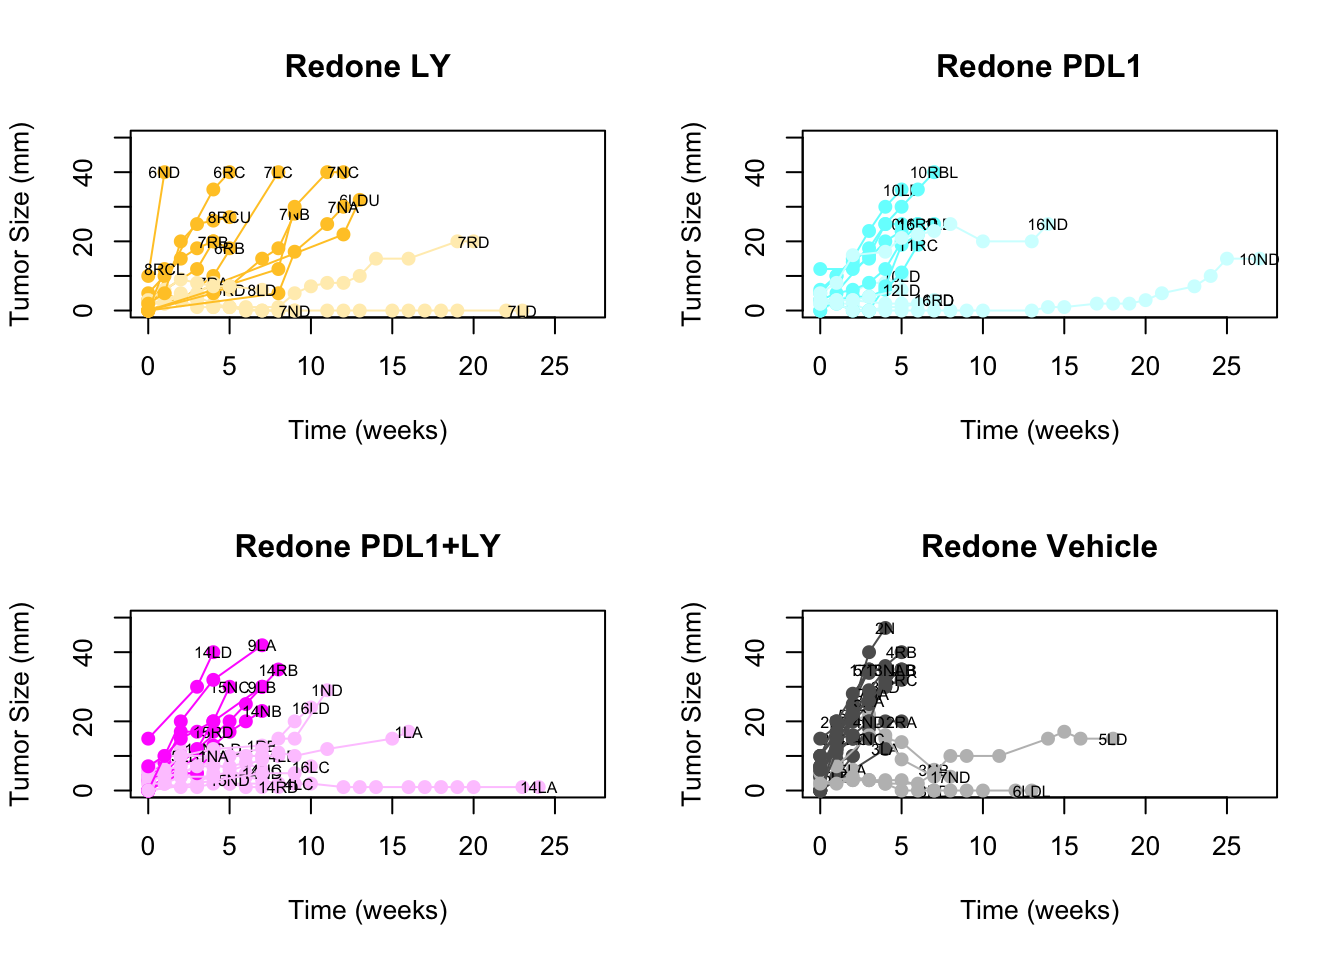
\includegraphics{RatDCIS-bookdown_files/figure-latex/unnamed-chunk-15-1.pdf}

As a sanity check, compare these growth rates with differences in tumour size at different time points:

\begin{itemize}
\tightlist
\item
  comparing the growth rate according to classifications (growing, stable)
\item
  tumor size at time of sacrifice
\item
  rate of tumor development from the time of NMU injection
\end{itemize}

\begin{verbatim}
## Warning in wilcox.test.default(x = c(3.54285714285714, 15, 20, 11.7, 5.8, :
## cannot compute exact p-value with ties
\end{verbatim}

\begin{verbatim}
## Warning in wilcox.test.default(x = c(20, 15, 20, 47, 30, 12, 32, 35, 4, : cannot
## compute exact p-value with ties
\end{verbatim}

\begin{verbatim}
## Warning in wilcox.test.default(x = c(0.238095238095238, 0.178571428571429, :
## cannot compute exact p-value with ties
\end{verbatim}

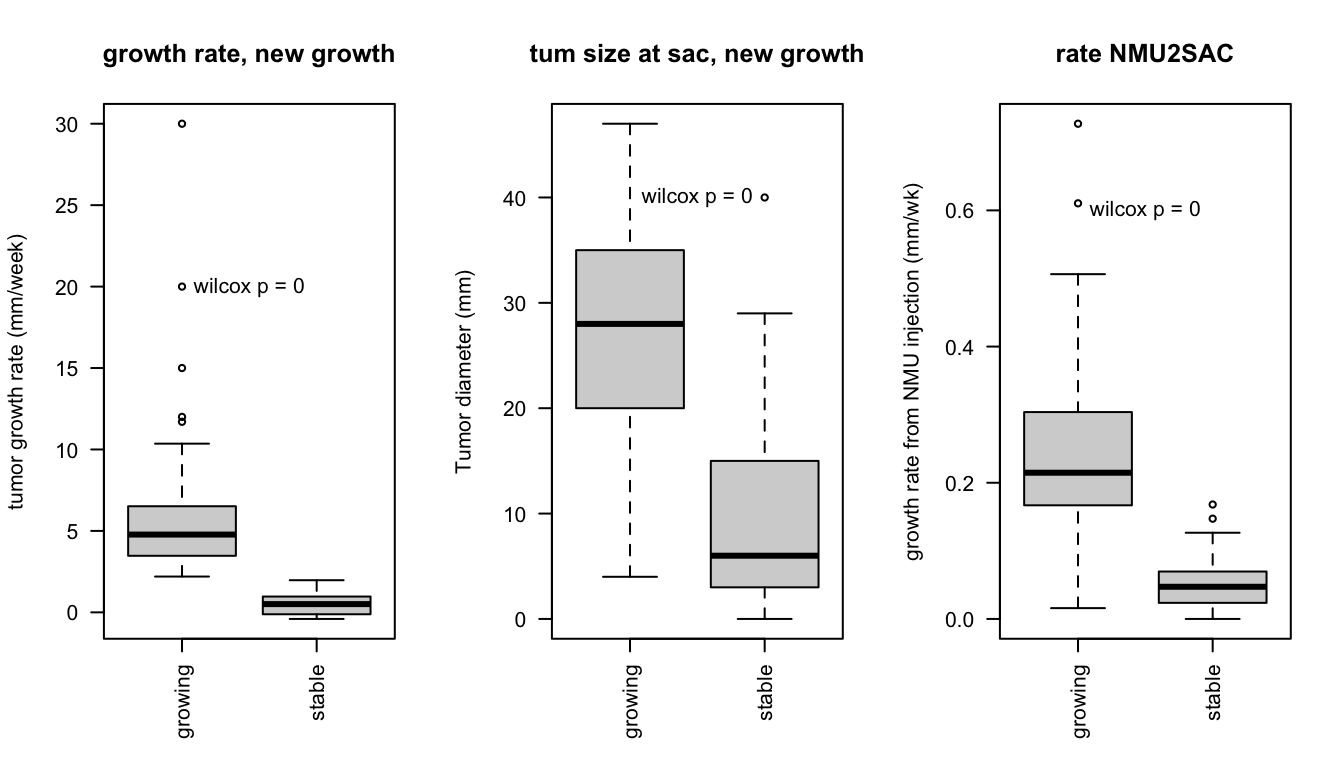
\includegraphics{RatDCIS-bookdown_files/figure-latex/unnamed-chunk-16-1.pdf}

Is there an association with treatment? Calculate below using chi-squared test:

\begin{verbatim}
## 
##  Pearson's Chi-squared test
## 
## data:  table(factor(d1$treatment), d1$growthrate_cutoff2)
## X-squared = 6.8181, df = 3, p-value = 0.07793
\end{verbatim}

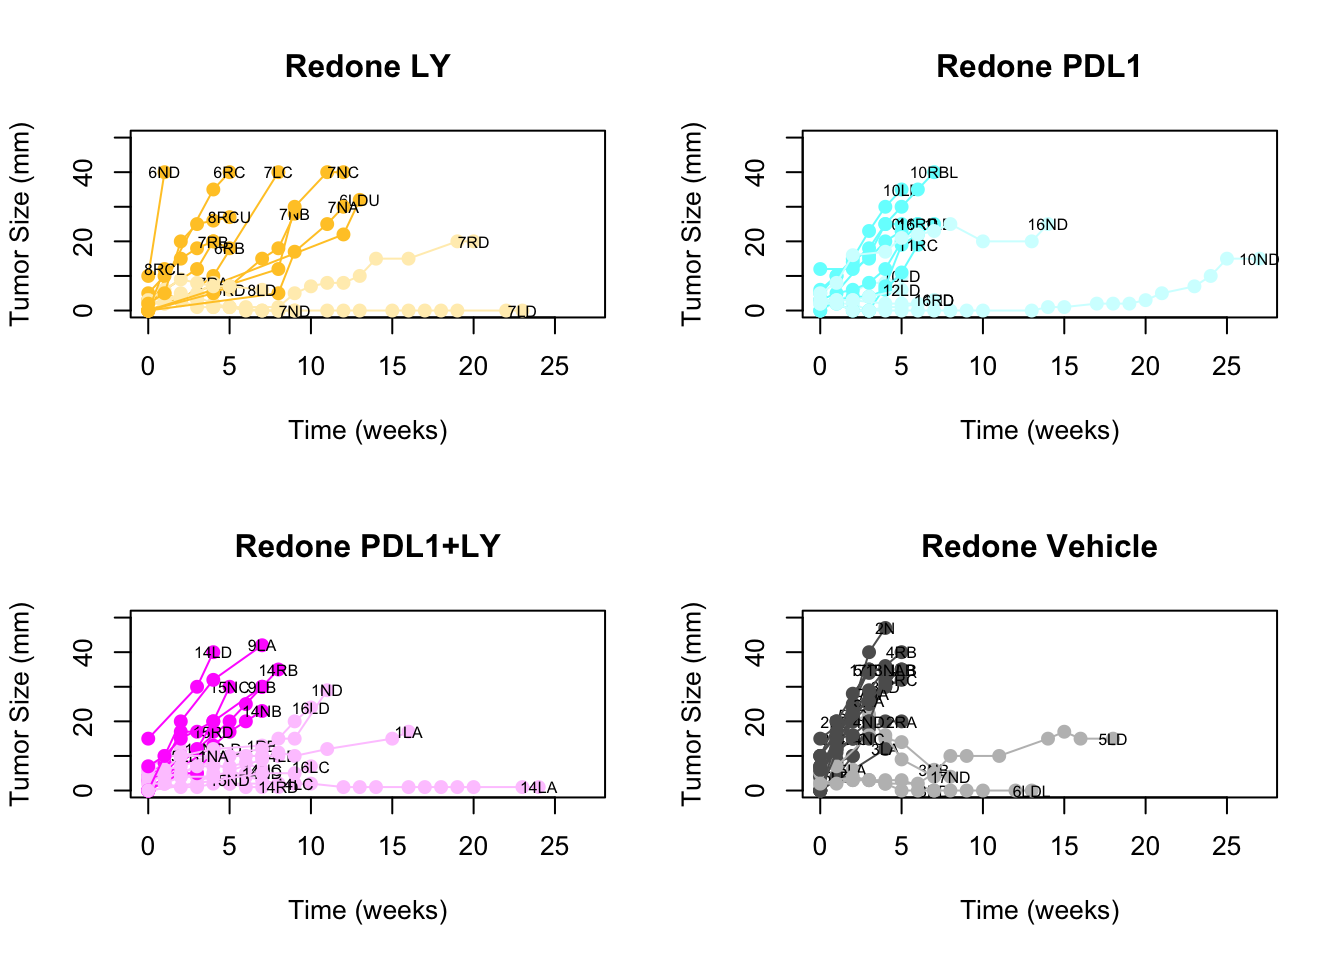
\includegraphics{RatDCIS-bookdown_files/figure-latex/unnamed-chunk-17-1.pdf}

Overall, it appears that there is an association between growth rate and treatment

\hypertarget{facs-data}{%
\section{FACS data}\label{facs-data}}

The immune (CD45) fractions from a number of samples were collected, and assessed using FACs. The major cell types detected are:

Leukocytes:

\begin{itemize}
\tightlist
\item
  Tregs
\item
  CD8 T cells
\item
  Thelper cells
\item
  B cells
\item
  NK T cells
\item
  gamma delta T cells
\end{itemize}

Myeloid cells:

\begin{itemize}
\tightlist
\item
  Macrophages M1
\item
  Macrophages M2
\item
  Dendritic cells
\item
  Monocytes
\item
  Neutrophils
\end{itemize}

We can look at the:

\begin{itemize}
\tightlist
\item
  types of cells
\item
  distributions
\end{itemize}

Note that in a number of samples the leukocyte population could not be inferred with confidence, and proportions are normalised to the myeloid population

\begin{verbatim}
##          type         11ND          8LD         8RCU         12LD 6RB 11RD
## 1  Leukocytes 913.84000000 379.56000000 829.57000000 298.83000000  NA   NA
## 2  leukocytes           NA           NA           NA           NA  NA   NA
## 3                       NA           NA           NA           NA  NA   NA
## 4          Th   0.18237328   0.12232585   0.12397989   0.05427835  NA   NA
## 5       Tregs   0.10207476   0.38225840   0.05701749   0.07030753  NA   NA
## 6 CD8 T cells   0.05586317   0.03293287   0.02488036   0.02399357  NA   NA
##           14ND         14NC          3NB          3RC         10LC         10RB
## 1 291.43000000 576.74000000 1.118820e+03 616.38000000 414.75000000 899.60000000
## 2           NA           NA           NA           NA           NA           NA
## 3           NA           NA           NA           NA           NA           NA
## 4   0.15032769   0.13704616 9.641408e-02   0.09800772   0.08323086   0.14899956
## 5   0.07030848   0.04386725 1.722261e-01   0.13929719   0.16072333   0.13873944
## 6   0.06811241   0.04036481 6.289662e-02   0.04382037   0.02013261   0.04357492
##           11LB         11RC 15LB 15NC 15RD 16LD 2RA 2RC 5NA 6RD 8RCL
## 1 1.243790e+03 204.89000000   NA   NA   NA   NA  NA  NA  NA  NA   NA
## 2           NA           NA   NA   NA   NA   NA  NA  NA  NA  NA   NA
## 3           NA           NA   NA   NA   NA   NA  NA  NA  NA  NA   NA
## 4 9.106039e-02   0.04543902   NA   NA   NA   NA  NA  NA  NA  NA   NA
## 5 2.633885e-02   0.02923520   NA   NA   NA   NA  NA  NA  NA  NA   NA
## 6 8.868057e-03   0.01883938   NA   NA   NA   NA  NA  NA  NA  NA   NA
\end{verbatim}

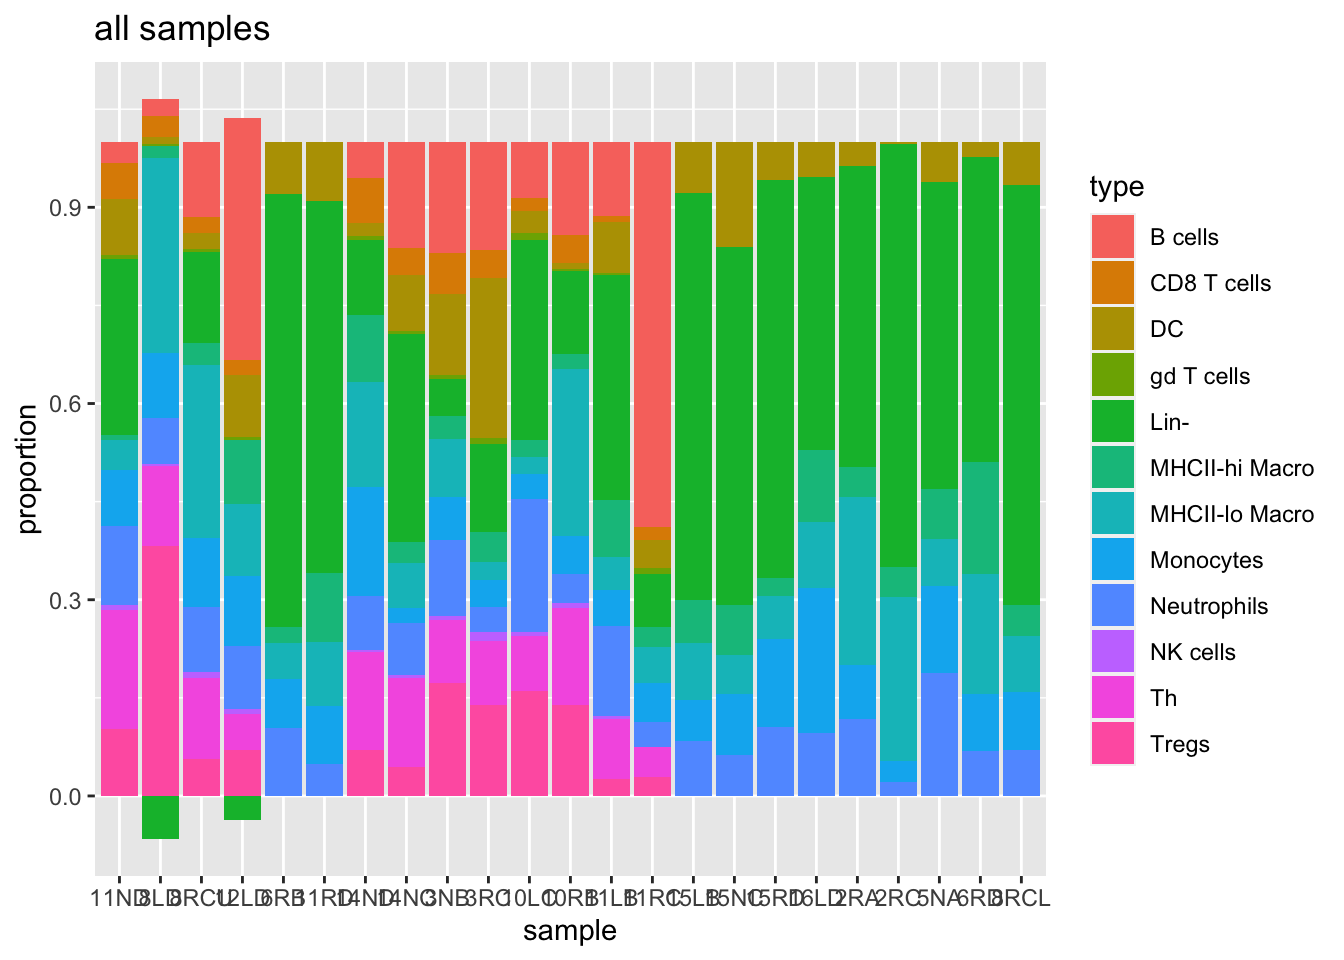
\includegraphics{RatDCIS-bookdown_files/figure-latex/unnamed-chunk-19-1.pdf}

We can look solely at the myeloid population (and normalise to this total), and color according to growth

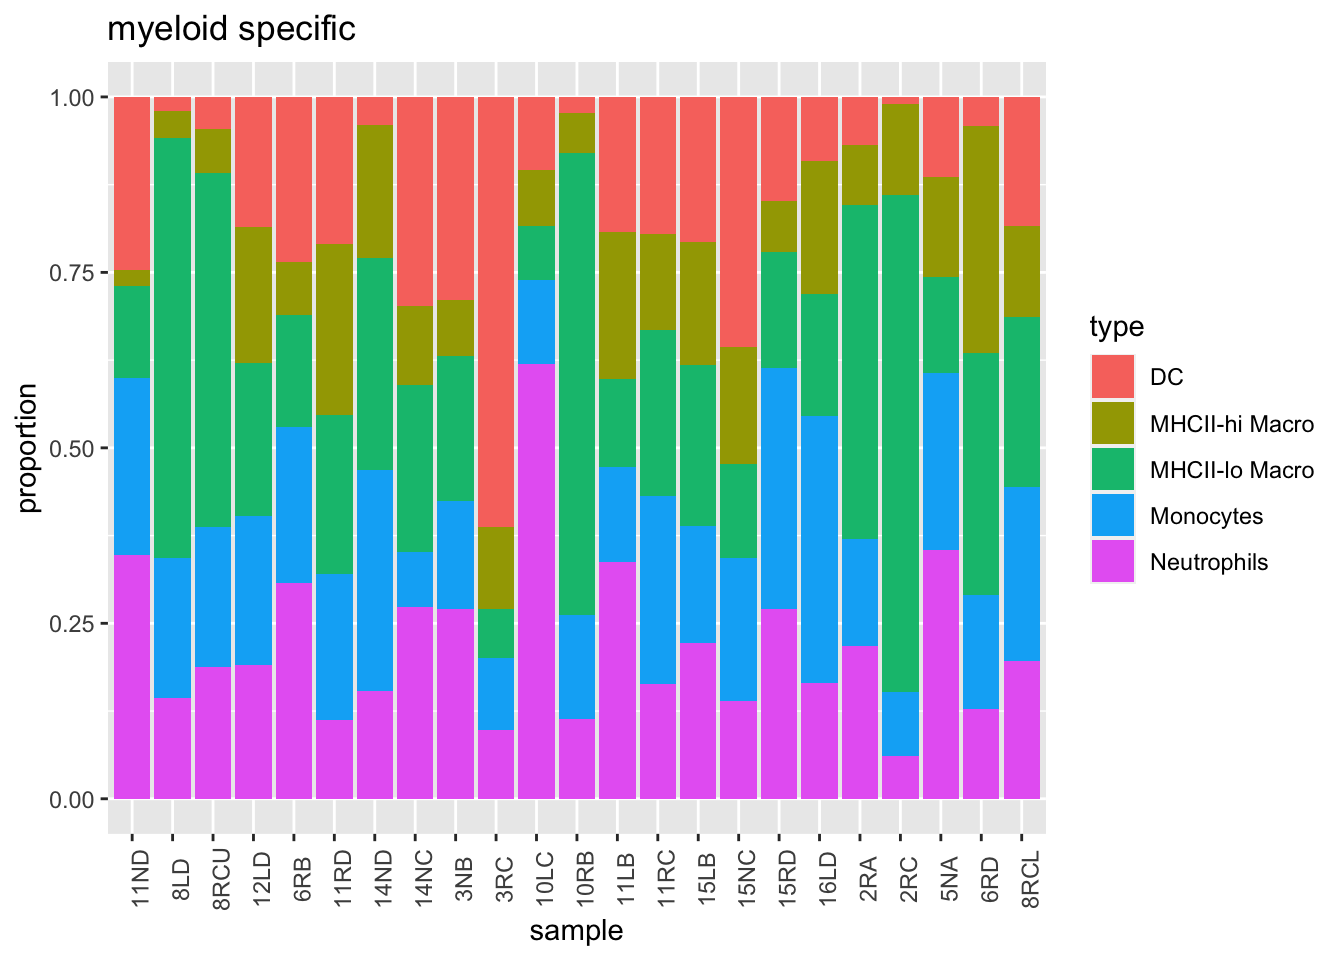
\includegraphics{RatDCIS-bookdown_files/figure-latex/unnamed-chunk-20-1.pdf}
Similarly, we can look at the leukocyte population. Note that the Treg population in some of these samples is very high.

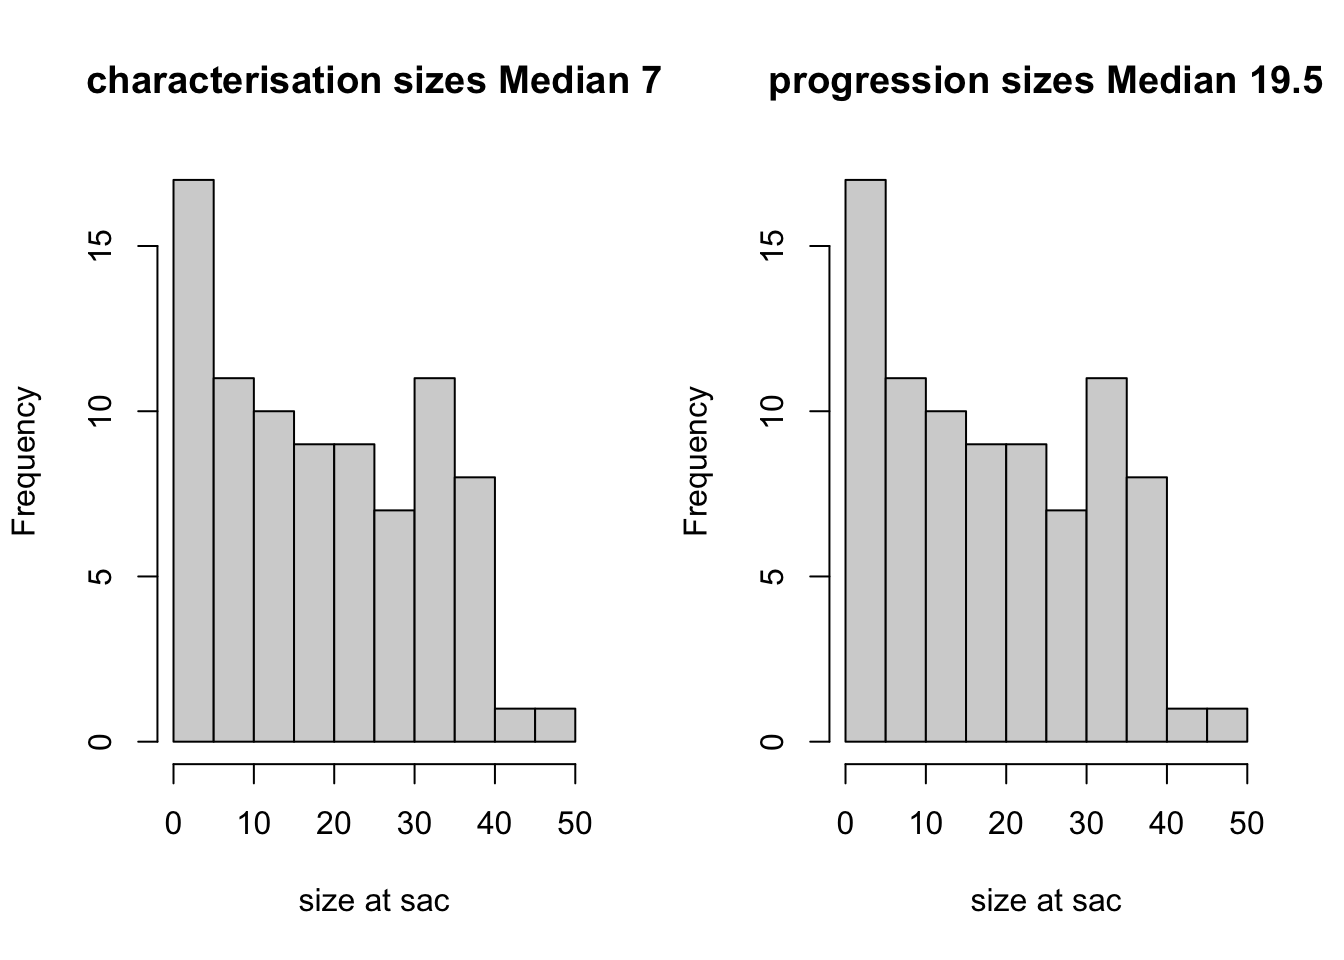
\includegraphics{RatDCIS-bookdown_files/figure-latex/unnamed-chunk-21-1.pdf}

\hypertarget{summary-table}{%
\section{Summary Table}\label{summary-table}}

Firstly, look at the total number of samples:

\begin{longtable}[]{@{}lll@{}}
\toprule
Feature & Levels & N\tabularnewline
\midrule
\endhead
Total No Tumors & All & 143\tabularnewline
- & Characterisation & 33\tabularnewline
- & Prevention & 8\tabularnewline
- & Progression & 84\tabularnewline
Total No Rats & All & 69\tabularnewline
- & Characterisation & 18\tabularnewline
- & Prevention & 8\tabularnewline
- & Progression & 42\tabularnewline
No tumours per rat & & 1.84 ( 1, 3)\tabularnewline
\bottomrule
\end{longtable}

\hypertarget{compare-the-characterisation-vs-progression-cohort}{%
\subsection{Compare the characterisation vs progression cohort}\label{compare-the-characterisation-vs-progression-cohort}}

\begin{longtable}[]{@{}llll@{}}
\toprule
Feature & Levels & Characterisation & Progression\tabularnewline
\midrule
\endhead
Total No tumours & & 59 & 102\tabularnewline
Treatments & Vehicle & 64 & 27\tabularnewline
- & Untreated & 4 &\tabularnewline
- & LY & & 17\tabularnewline
- & PDL1 & & 17\tabularnewline
- & PDL1+LY & & 23\tabularnewline
- & NA & 18 & 18\tabularnewline
Histology & diff. adenocarcinomas & 41 & 76\tabularnewline
- & mucinous carcinoma & 0 & 3\tabularnewline
- & Fibroadenoma & 0 & 4\tabularnewline
- & NA & 18 & 19\tabularnewline
Age Injection & 32-36 & 8 & 84\tabularnewline
- & 35 & 27 & 0\tabularnewline
- & 49 & 6 & 0\tabularnewline
- & NA & 18 & 18\tabularnewline
Time (days) & NMU 2 Sac & 98.59 (54, 160) & 149.37 (79, 248.7)\tabularnewline
- & Cases with NA & 30 & 18\tabularnewline
- & NMU 2 Tumor & & 100.62 (44.2, 182.7)\tabularnewline
- & Cases with NA & 59 & 18\tabularnewline
- & Tum Spec Surv & & 48.75 (9.5, 92)\tabularnewline
- & Cases with NA & 59 & 18\tabularnewline
Growth Rate/Size (mm) & overall size @ sac & 6.67 (1.4, 12.4) & 19.52 (3, 40)\tabularnewline
- & Growing No. & & 47\tabularnewline
- & Growing size @ sac & & 27.7 15, 28, 40\tabularnewline
- & Stable & & 31\tabularnewline
- & Stable size @ sac & & 9.58 (1, 6, 24)\tabularnewline
- & NA & 59 & 24\tabularnewline
Spatial Pattern & & &\tabularnewline
- & Infiltrating & 0 & 26\tabularnewline
- & Restricted & 0 & 33\tabularnewline
- & NA & 59 & 43\tabularnewline
RNA samples & any fraction & 14 & 46\tabularnewline
- & Ep & 14 & 21\tabularnewline
- & DN & 0 & 33\tabularnewline
- & CD45 & 10 & 36\tabularnewline
Imaging Data & No tumors & & 64\tabularnewline
- & No tumors with RNA & & 38\tabularnewline
FACS data & Comprehensive & & 22\tabularnewline
- & EpCAM/CD45 & 0 & 82\tabularnewline
\bottomrule
\end{longtable}

{
TO INCLUDE:
- trichrome data?
}

\hypertarget{summary-of-the-rna-data}{%
\subsection{Summary of the RNA data}\label{summary-of-the-rna-data}}

Below is a table of the samples with RNA information

\begin{longtable}[]{@{}llll@{}}
\toprule
Feature & Levels & Characterisation & Progression\tabularnewline
\midrule
\endhead
RNA samples & any fraction & 14 & 46\tabularnewline
- & Ep & 14 & 21\tabularnewline
- & DN & 0 & 33\tabularnewline
- & CD45 & 10 & 36\tabularnewline
Treatments Char/Prev & Vehicle & 13 & 15\tabularnewline
- & Untreat (char) & 1 &\tabularnewline
- & LY & & 9\tabularnewline
- & PDL1 & & 11\tabularnewline
- & PDL1+LY & & 11\tabularnewline
- & NA & 0 & 0\tabularnewline
Time & NMU 2 Sac & 106.9 (54.9, 160) & 113.85 (79, 166)\tabularnewline
Growth Rate/Size (mm) & overall size @ sac & 7.1 (3.9, 12.2) & 21.96 (6, 37.5)\tabularnewline
- & Growing No. & & 33\tabularnewline
- & Growing size @ sac & & 27.64 15, 28, 40\tabularnewline
- & Stable & & 12\tabularnewline
- & Stable size @ sac & & 7.17 (3.1, 6, 9.7)\tabularnewline
- & NA & 14 & 1\tabularnewline
Growth and Treatment: comparing small/stable vs large/growing & & &\tabularnewline
Vehicle & N s/l & & 2, 13\tabularnewline
LY & N s/l & & 2, 7\tabularnewline
PDL1 and Treatment & N s/l & & 4, 6\tabularnewline
PDL1+LY & N s/l & & 4, 7\tabularnewline
\bottomrule
\end{longtable}

\hypertarget{whole-slide-imaging}{%
\chapter{Whole-slide imaging}\label{whole-slide-imaging}}

In this section, we will be looking at the composition and spatial distribution of cells in whole slide images. These sections have previously been assessed using an {external script. Save this somewhere }

The following markers have been used:

\begin{itemize}
\tightlist
\item
  EpCAM (tumor cells)
\item
  SMA (fibroblasts or myeopithelial cells)
\item
  CD8 (T cells)
\end{itemize}

Note that in some images a double positive EpCAM+/SMA+ population exists. Some CD8 cells have Epcam+ or SMA+ staining, however, we consider all of these to be simply CD8+

\hypertarget{associate-the-frequencies-with-other-data-types}{%
\section{Associate the frequencies with other data types}\label{associate-the-frequencies-with-other-data-types}}

Note there are 47 samples with imaging data. 33 of these samples have FACS data, manual counts and TIMER scores

Correlate the following information:

\begin{itemize}
\tightlist
\item
  ``CD8.WSI'': CD8 total counts
\item
  ``CD8Frac.WSI'': CD8 fraction (normalised by cell count)
\item
  ``CD8\_EPorSMARatio.WSI'': CD8/EP+SMA ratio (any EpCAM or SMA + cell)
\item
  ``CD8\_AnySMARatio.WSI'': CD8/Any EPcam+ cell
\item
  ``CD8\_EPRatio.WSI'': CD8 to EpCAM+SMA- ratio
\item
  ``CD8normTumSize'': normalised CD8 counts per mm of tumor size at sac
\item
  ``CD8.EpBoundingBox'': approx area per CD8 cell (density)
\end{itemize}

{
UPDATE THE CIBERSORT INFORMATION. }

Below are heatmaps which show the correlation between two variables (red is correlated and blue is anti-correlated), and the p.value is indicated in the middle of the square.

It appears that CD8 whole-slide imaging associates well with:

\begin{itemize}
\tightlist
\item
  FACS data (both CD8 and CD45)
\item
  Manual scoring (Fig 4) of CD8 cells
\item
  Some CD8 gene signature scores (mainly in EPC, TIMER)
\end{itemize}

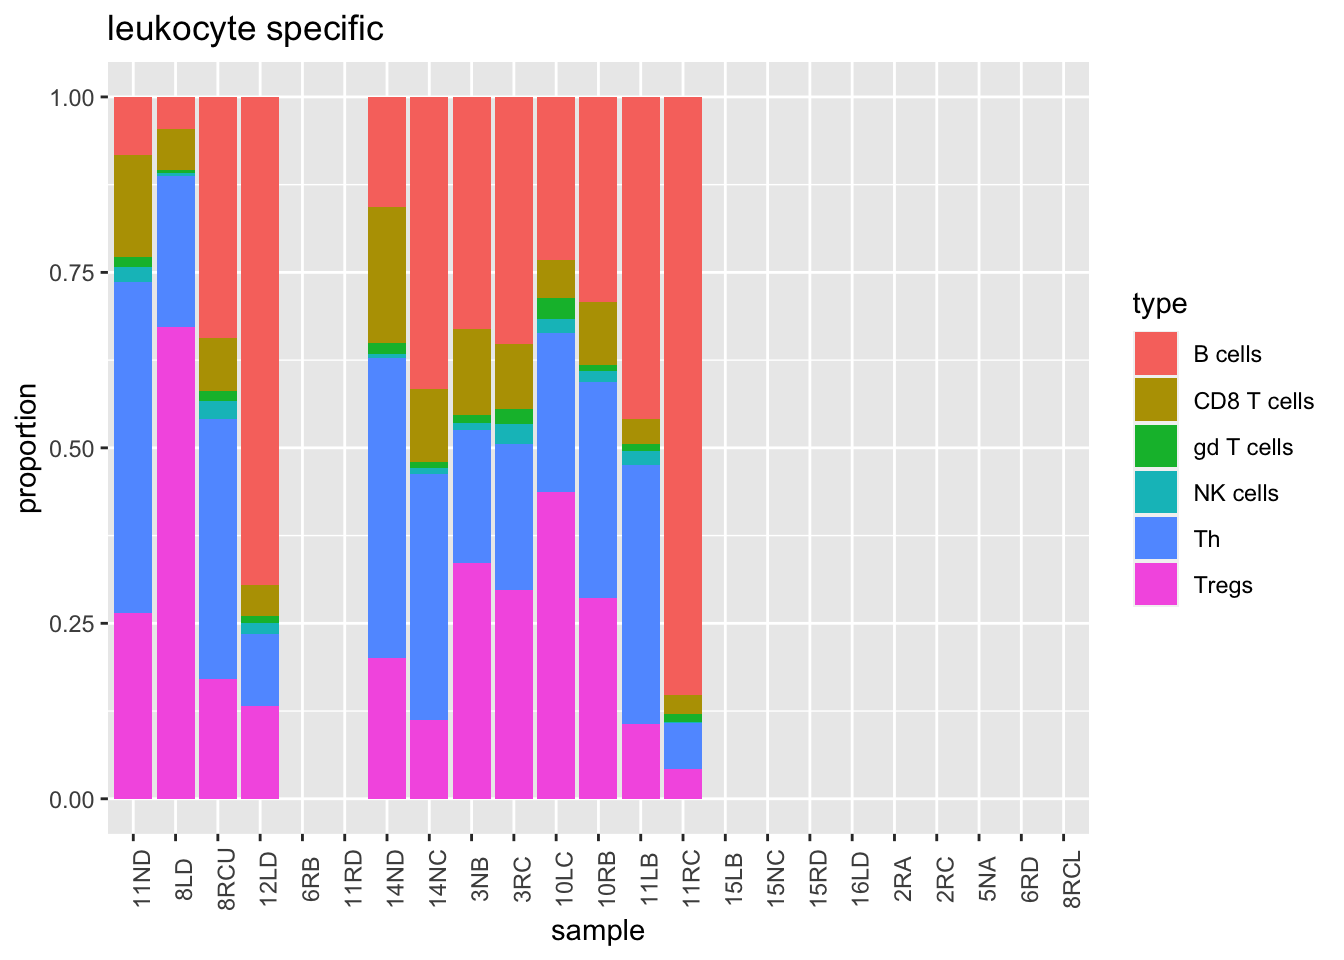
\includegraphics{RatDCIS-bookdown_files/figure-latex/unnamed-chunk-25-1.pdf} 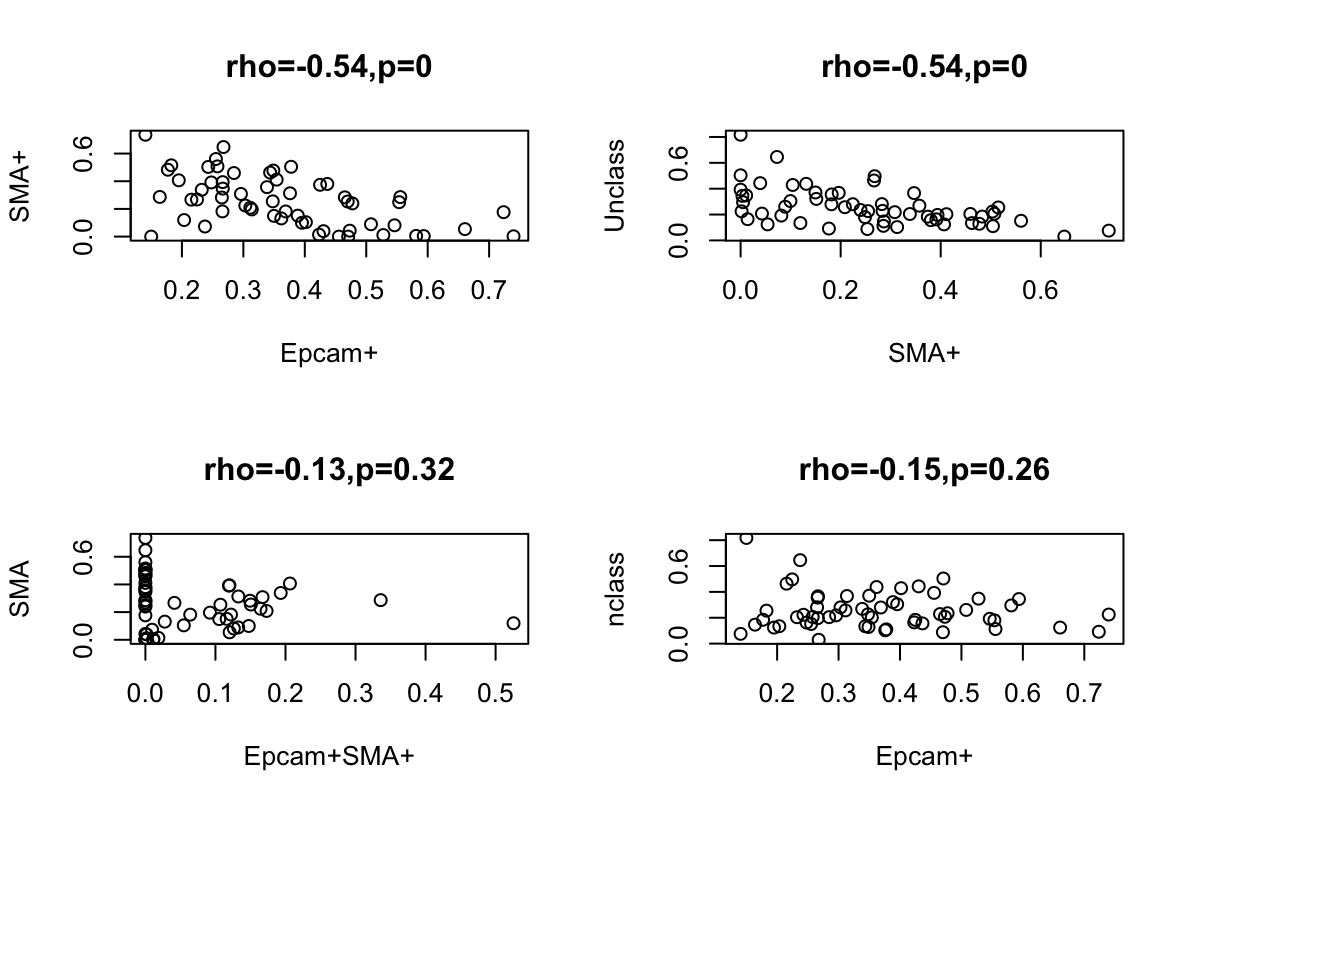
\includegraphics{RatDCIS-bookdown_files/figure-latex/unnamed-chunk-25-2.pdf}

\hypertarget{cellular-composition}{%
\section{Cellular composition}\label{cellular-composition}}

Here, we look at the raw distributions of the different cell types and see if there are associations with:

\begin{itemize}
\tightlist
\item
  tumor size
\item
  growth rate
\item
  growth rate (categorical)
\item
  treatment
\item
  stromal restricted or infiltrating
\end{itemize}

Below are the total cell counts:

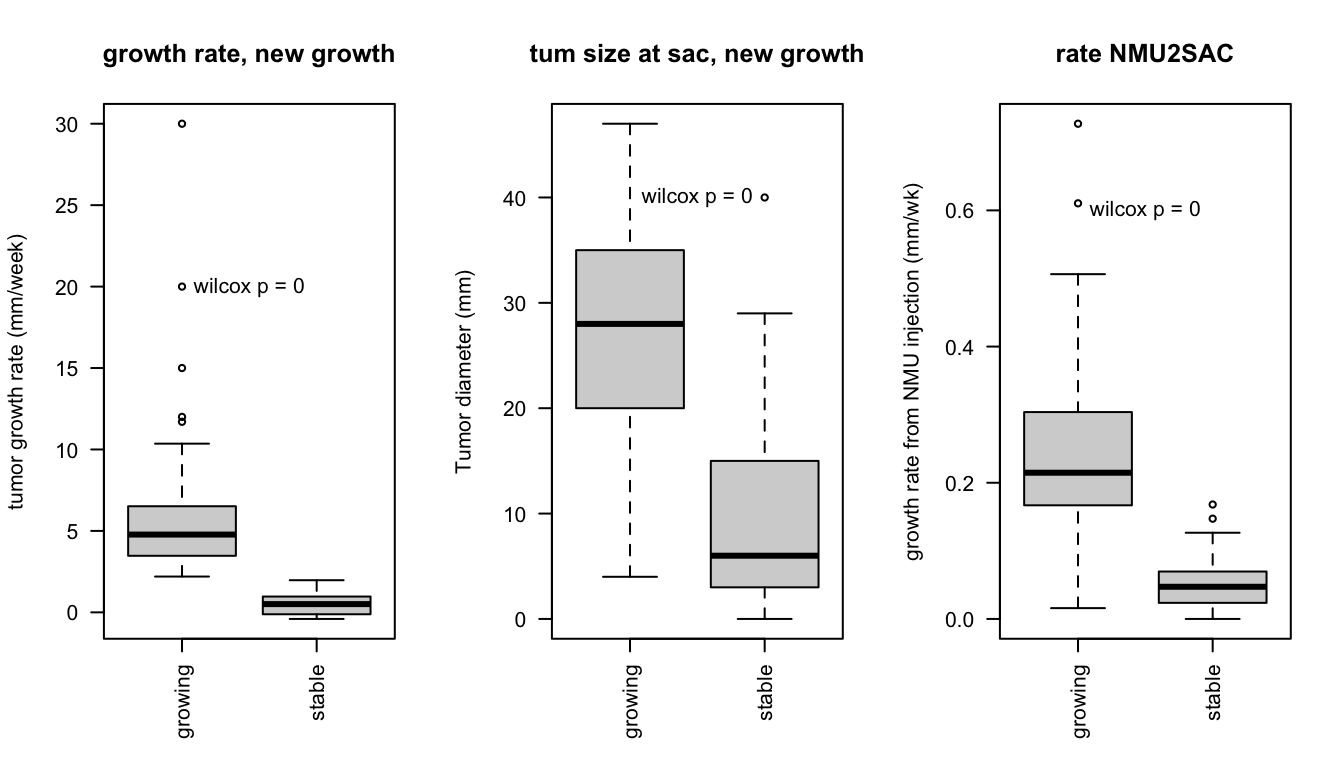
\includegraphics{RatDCIS-bookdown_files/figure-latex/unnamed-chunk-27-1.pdf} 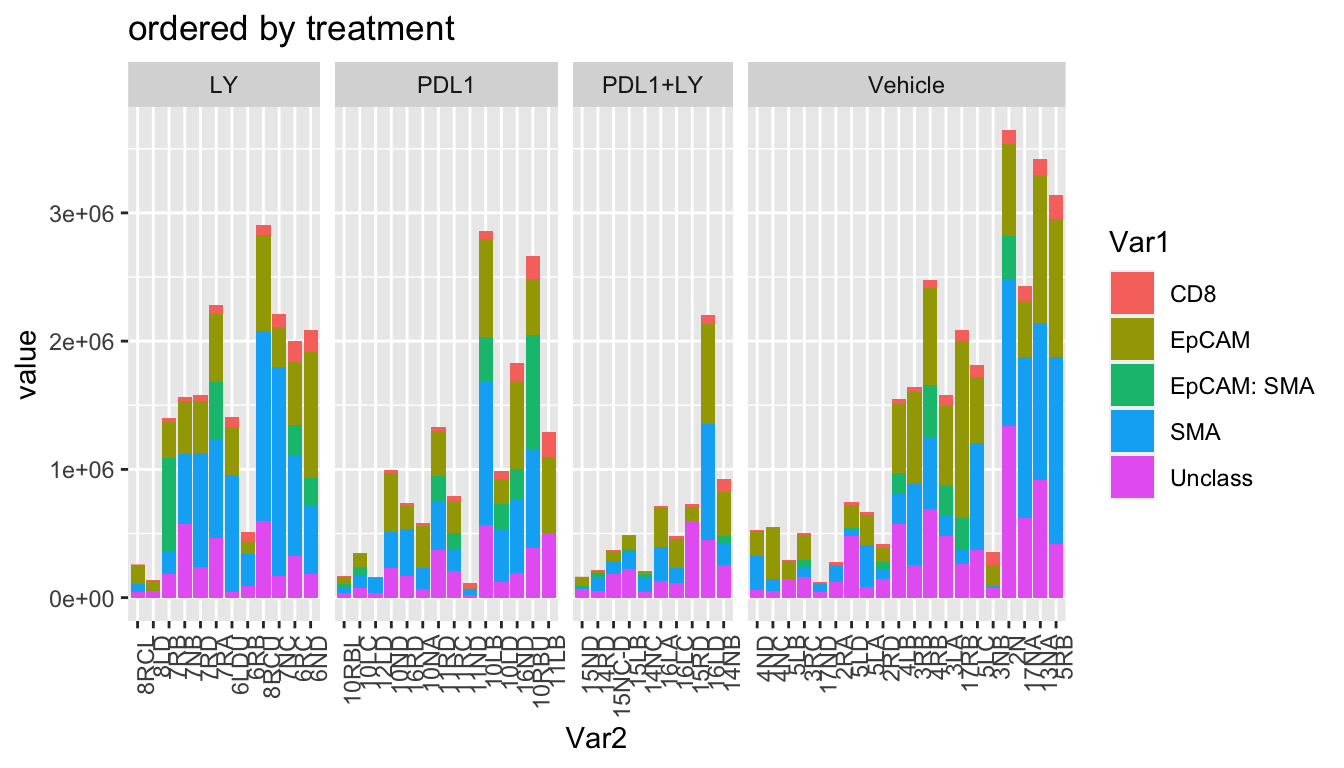
\includegraphics{RatDCIS-bookdown_files/figure-latex/unnamed-chunk-27-2.pdf} 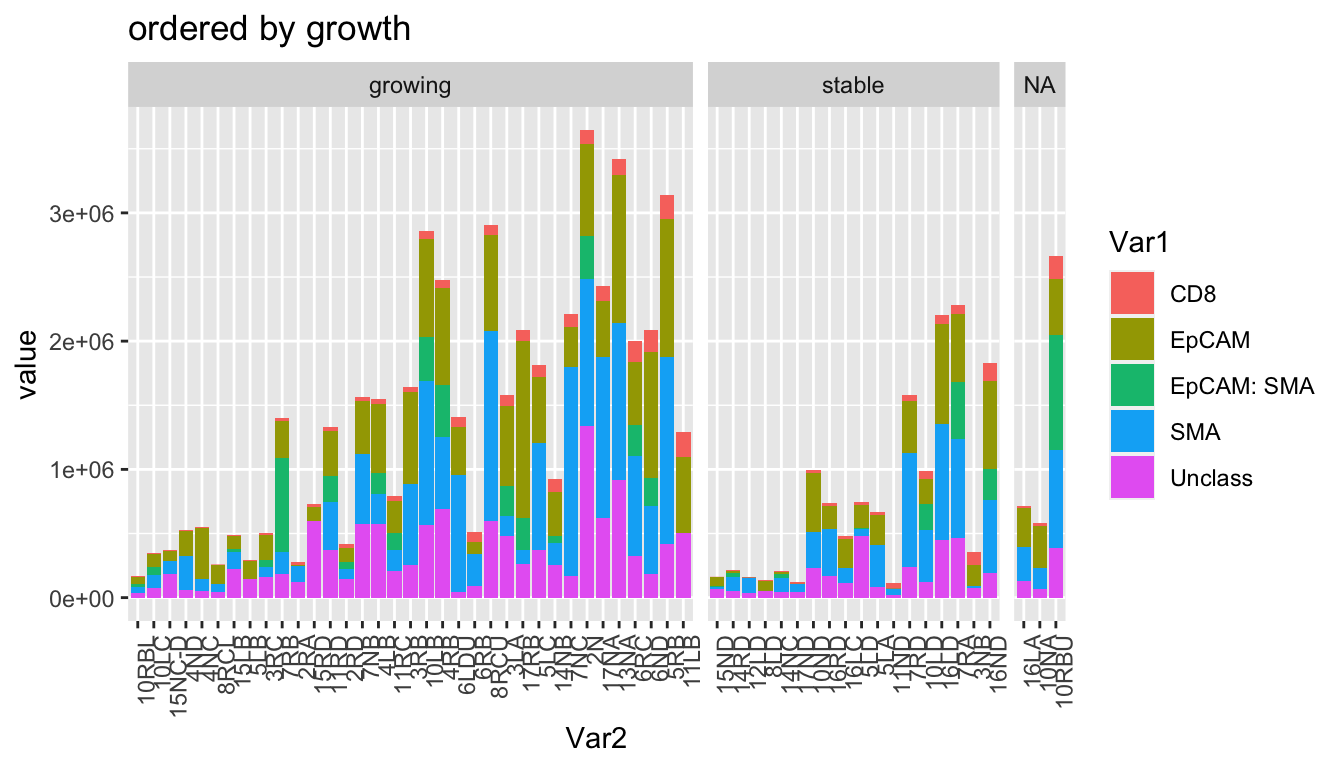
\includegraphics{RatDCIS-bookdown_files/figure-latex/unnamed-chunk-27-3.pdf}

Here, the same data is shown and normalised according to total cell count:

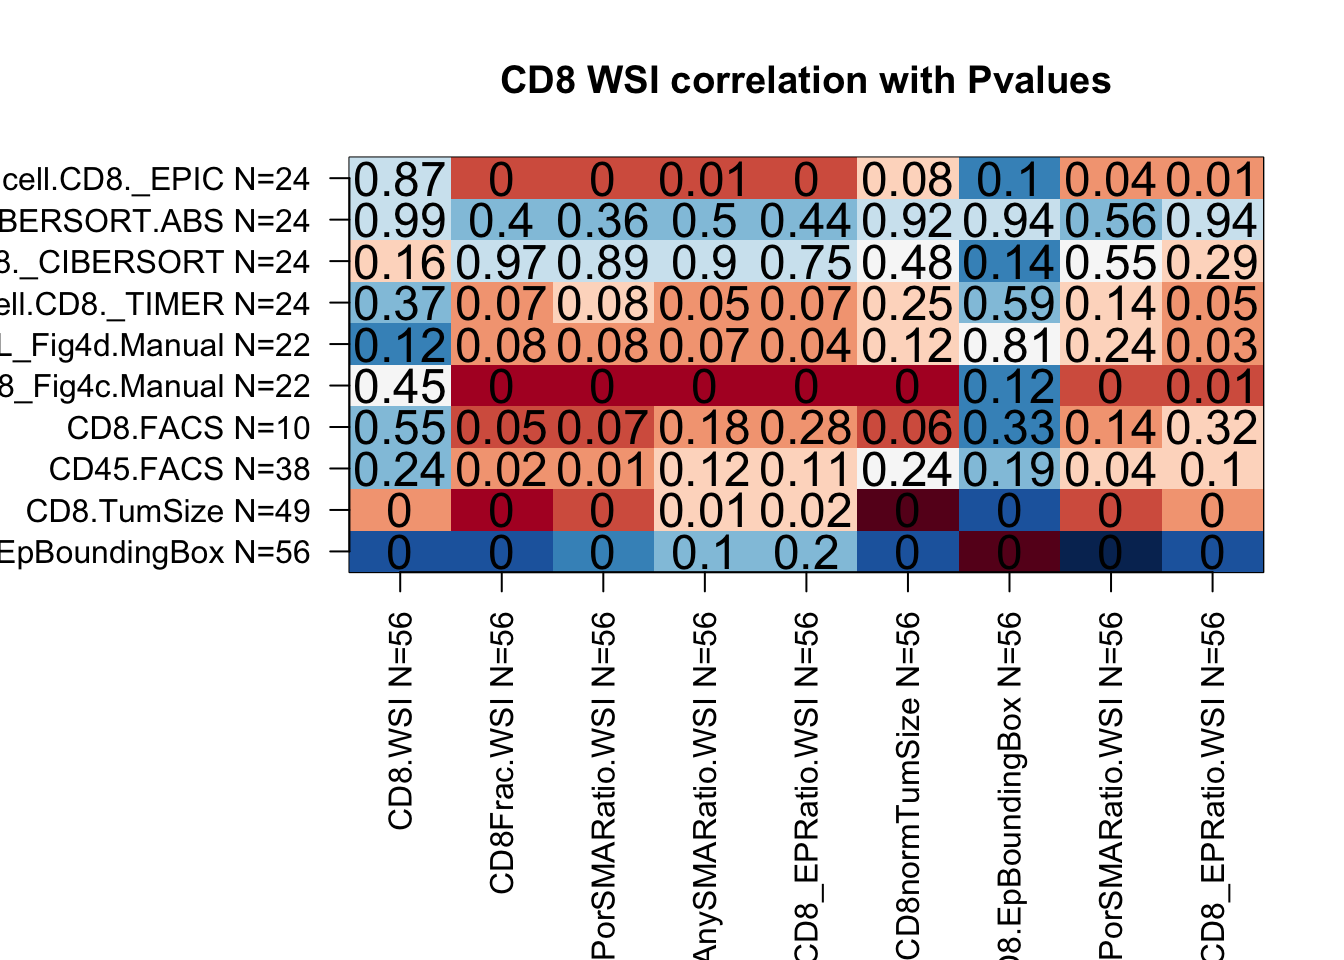
\includegraphics{RatDCIS-bookdown_files/figure-latex/unnamed-chunk-28-1.pdf} 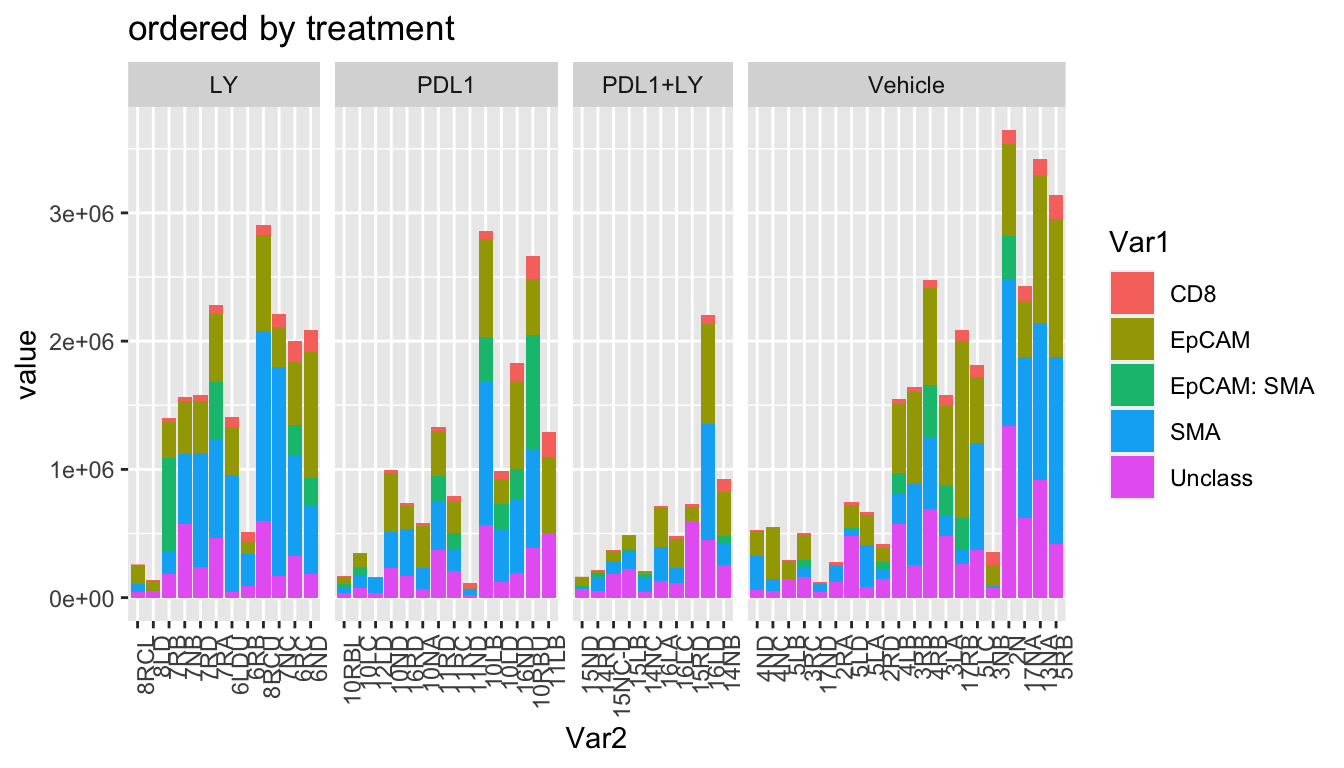
\includegraphics{RatDCIS-bookdown_files/figure-latex/unnamed-chunk-28-2.pdf} 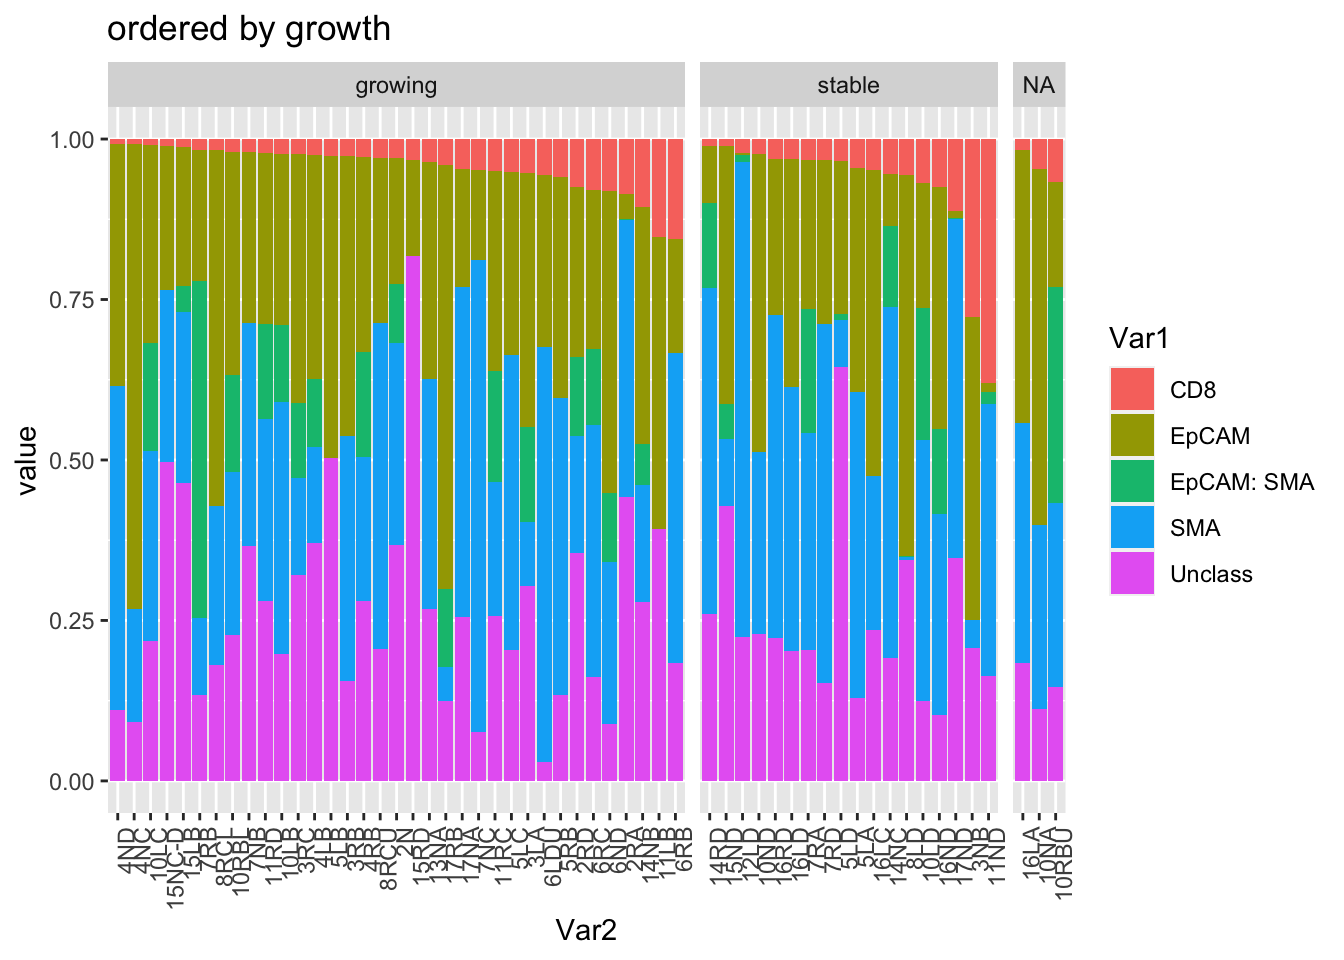
\includegraphics{RatDCIS-bookdown_files/figure-latex/unnamed-chunk-28-3.pdf}

\hypertarget{associate-composition-with-other-covariates}{%
\section{Associate composition with other covariates}\label{associate-composition-with-other-covariates}}

We can collapse the above data into boxplots to see if there is an association with treatments, performed using non-parametric wilcoxon test.

Compared to the vehicle, LY treated samples have a lower ``stromal'' fraction (unclassed DAPI+ cells) and PDL1 treated samples are more likely to have a EpCAM+SMA+ double positive fraction

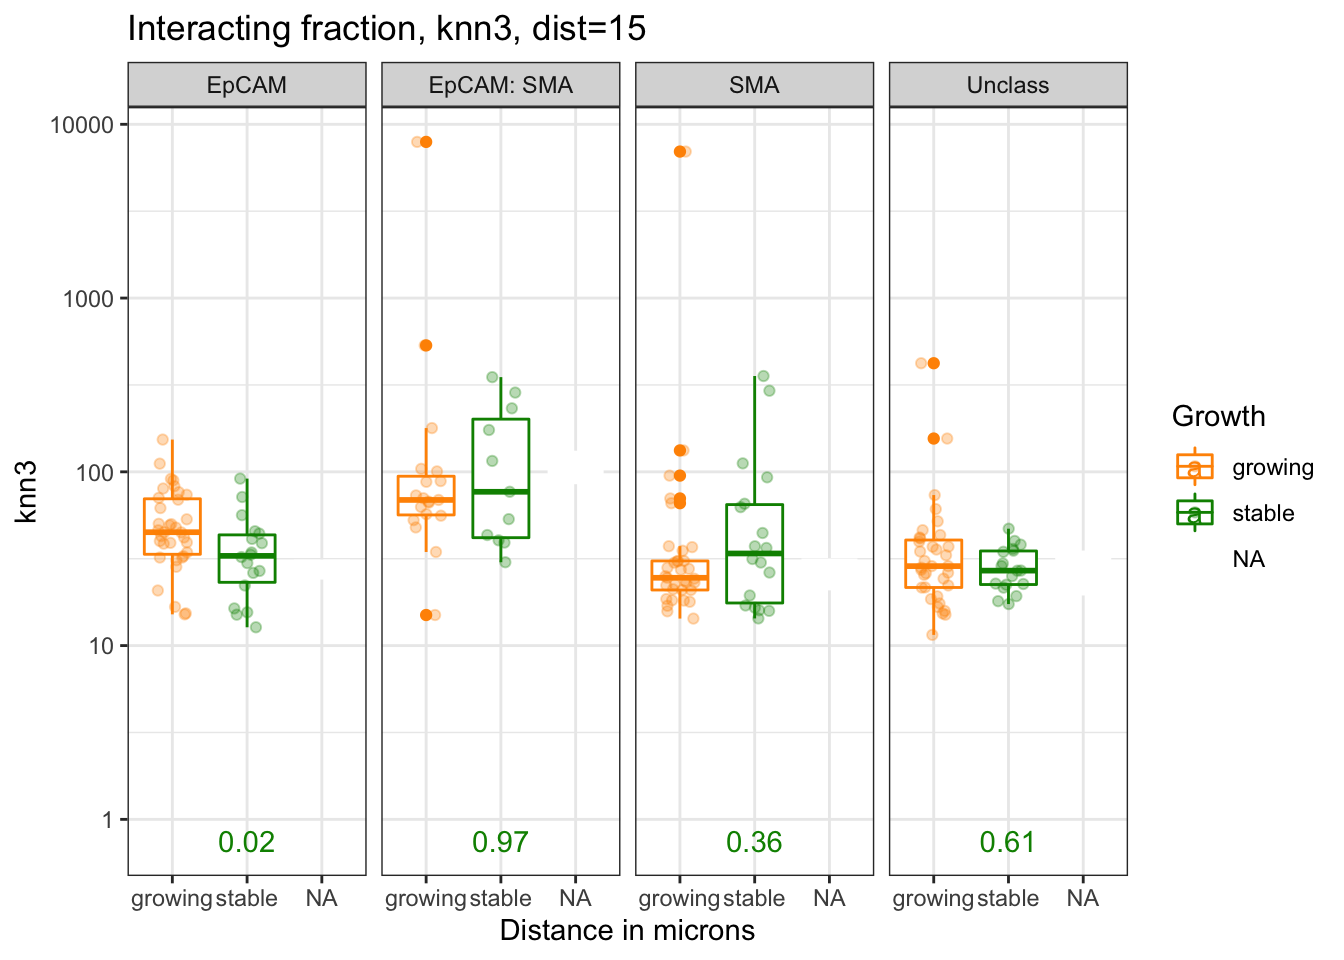
\includegraphics{RatDCIS-bookdown_files/figure-latex/unnamed-chunk-29-1.pdf}

When comparing these fractions to growth, there is no association:

\begin{verbatim}
## Warning in wilcox.test.default(Cdata[Cdata$Growth2 == "growing", i],
## Cdata[Cdata$Growth2 == : cannot compute exact p-value with ties

## Warning in wilcox.test.default(Cdata[Cdata$Growth2 == "growing", i],
## Cdata[Cdata$Growth2 == : cannot compute exact p-value with ties
\end{verbatim}

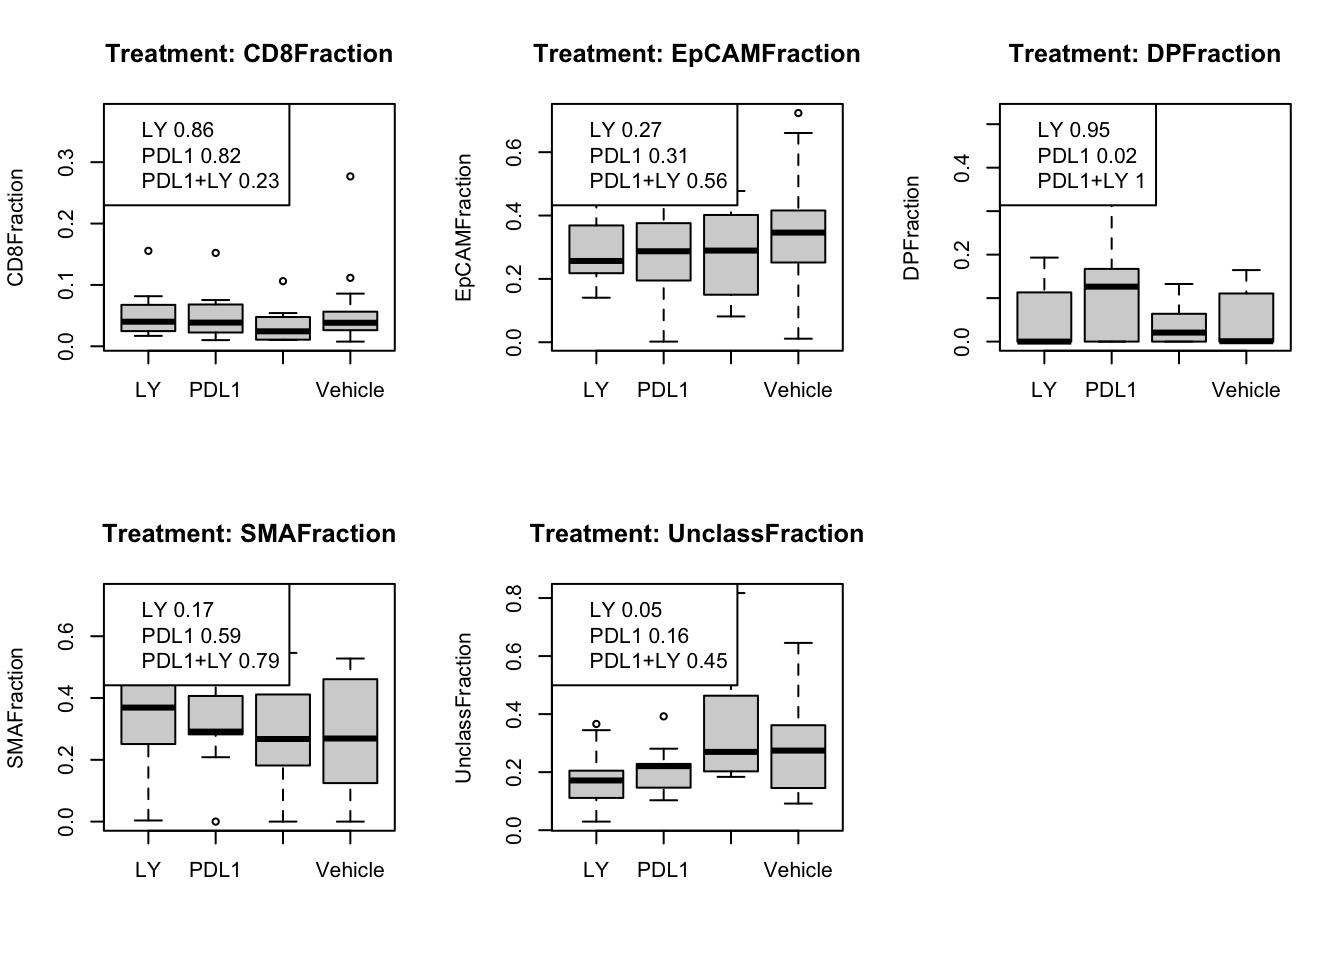
\includegraphics{RatDCIS-bookdown_files/figure-latex/unnamed-chunk-30-1.pdf}

Nor is there any association with whether a sample is ``immune infiltrated'' or not (by manual inspection)

\begin{verbatim}
## Warning in wilcox.test.default(Cdata[Cdata$InfiltratingVsRestricted ==
## "Infiltrating", : cannot compute exact p-value with ties

## Warning in wilcox.test.default(Cdata[Cdata$InfiltratingVsRestricted ==
## "Infiltrating", : cannot compute exact p-value with ties
\end{verbatim}

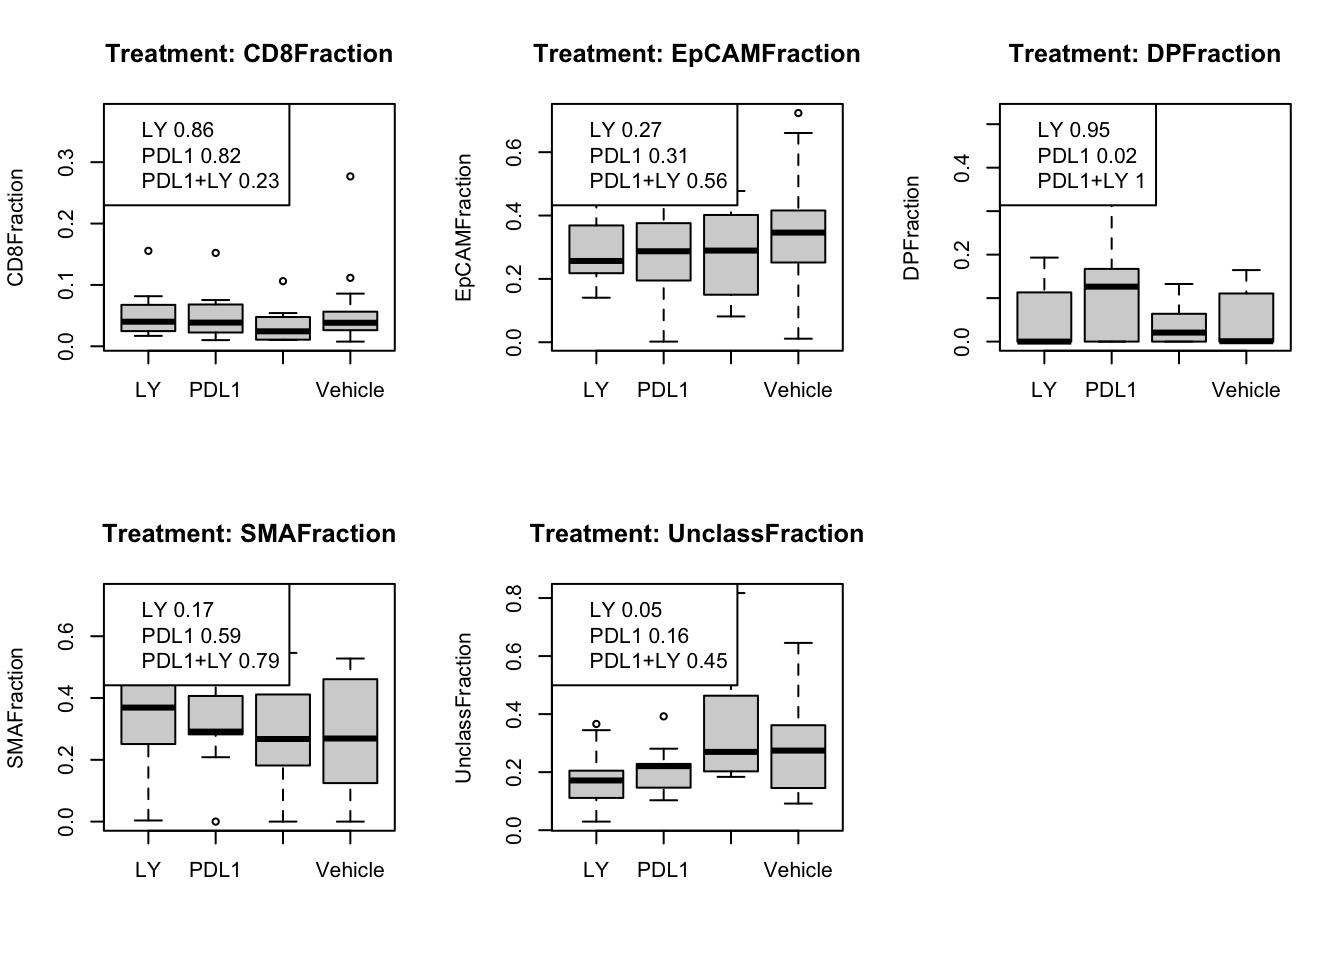
\includegraphics{RatDCIS-bookdown_files/figure-latex/unnamed-chunk-31-1.pdf}

We can also use linear regression models to assess:

\begin{itemize}
\tightlist
\item
  correlation between growth rate and cell fractions (no associations)
\item
  correlation between final tumor size and cell fractions (no association)
\end{itemize}

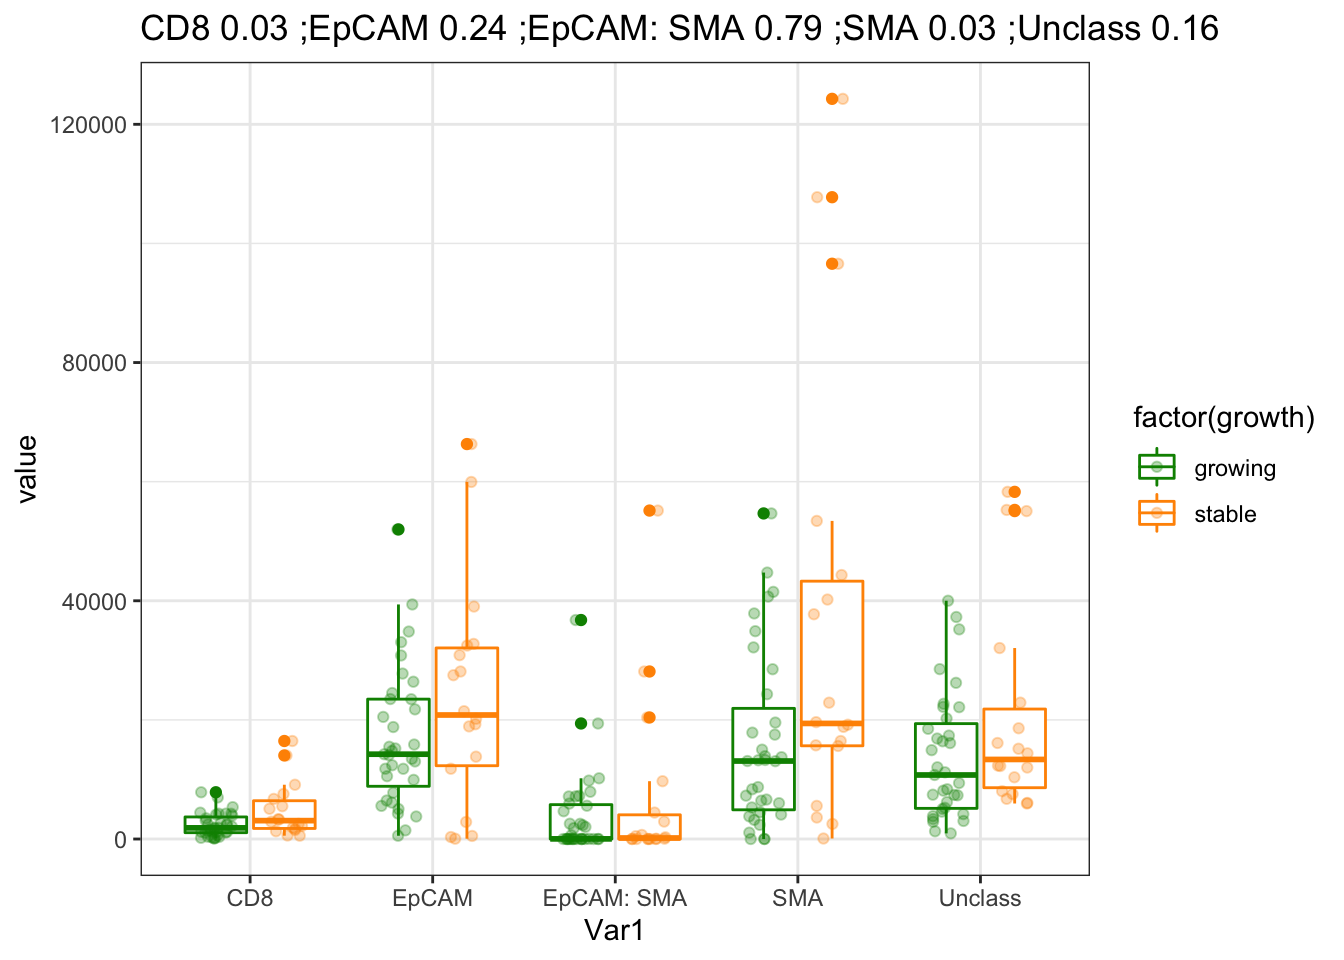
\includegraphics{RatDCIS-bookdown_files/figure-latex/unnamed-chunk-32-1.pdf} 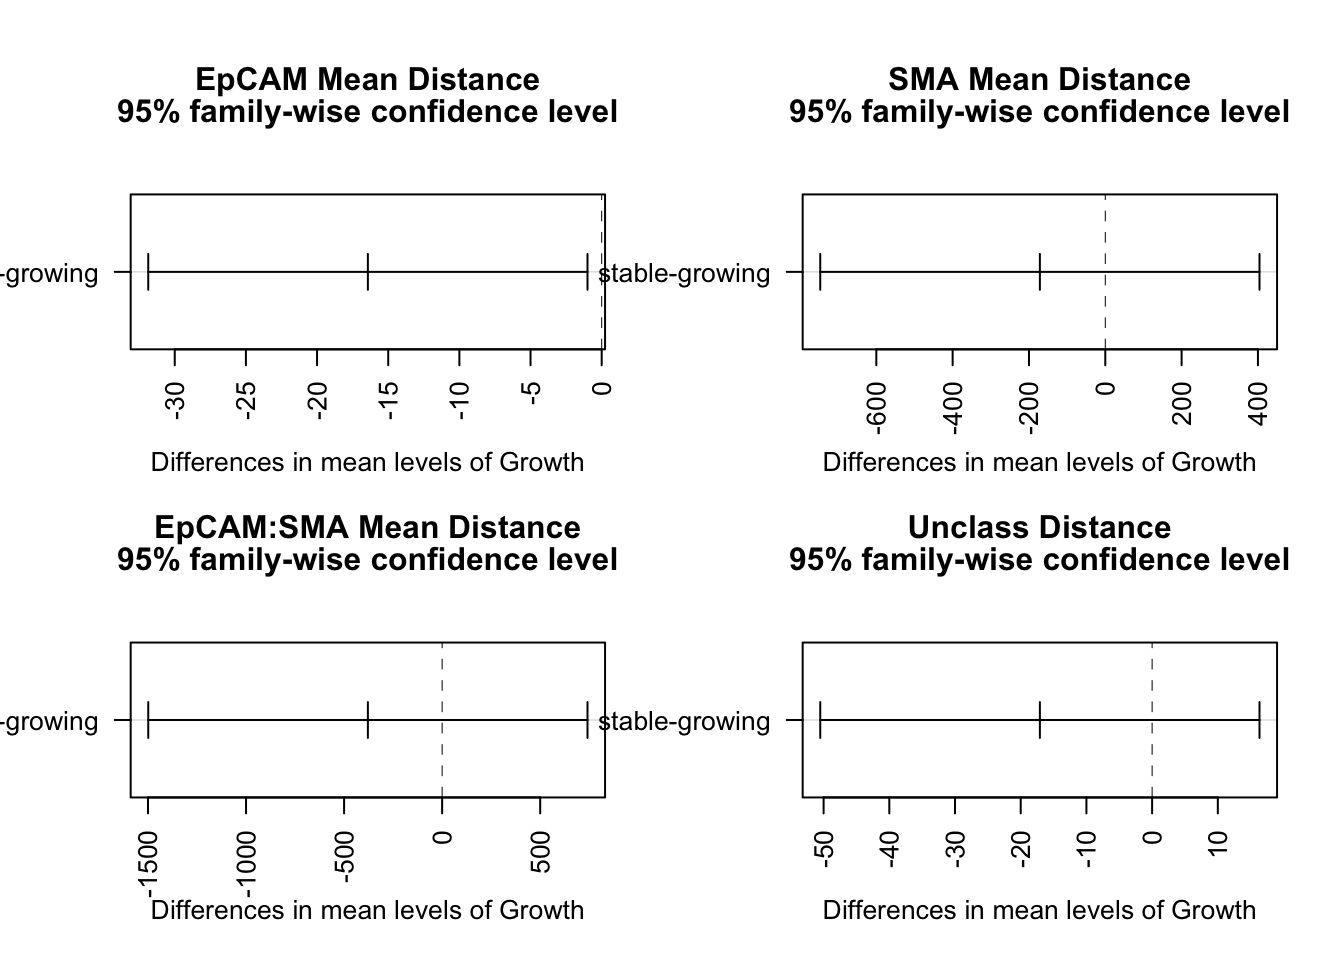
\includegraphics{RatDCIS-bookdown_files/figure-latex/unnamed-chunk-32-2.pdf}

\hypertarget{estimate-tumor-size}{%
\section{Estimate tumor size}\label{estimate-tumor-size}}

Using WSI data, we can estimate a tumor size for each tissue sample and compare to the final tumor sizes. This will be based on the distribution of EpCAM+ cells.
This estimate is also used to normalise CD8 counts earlier on.

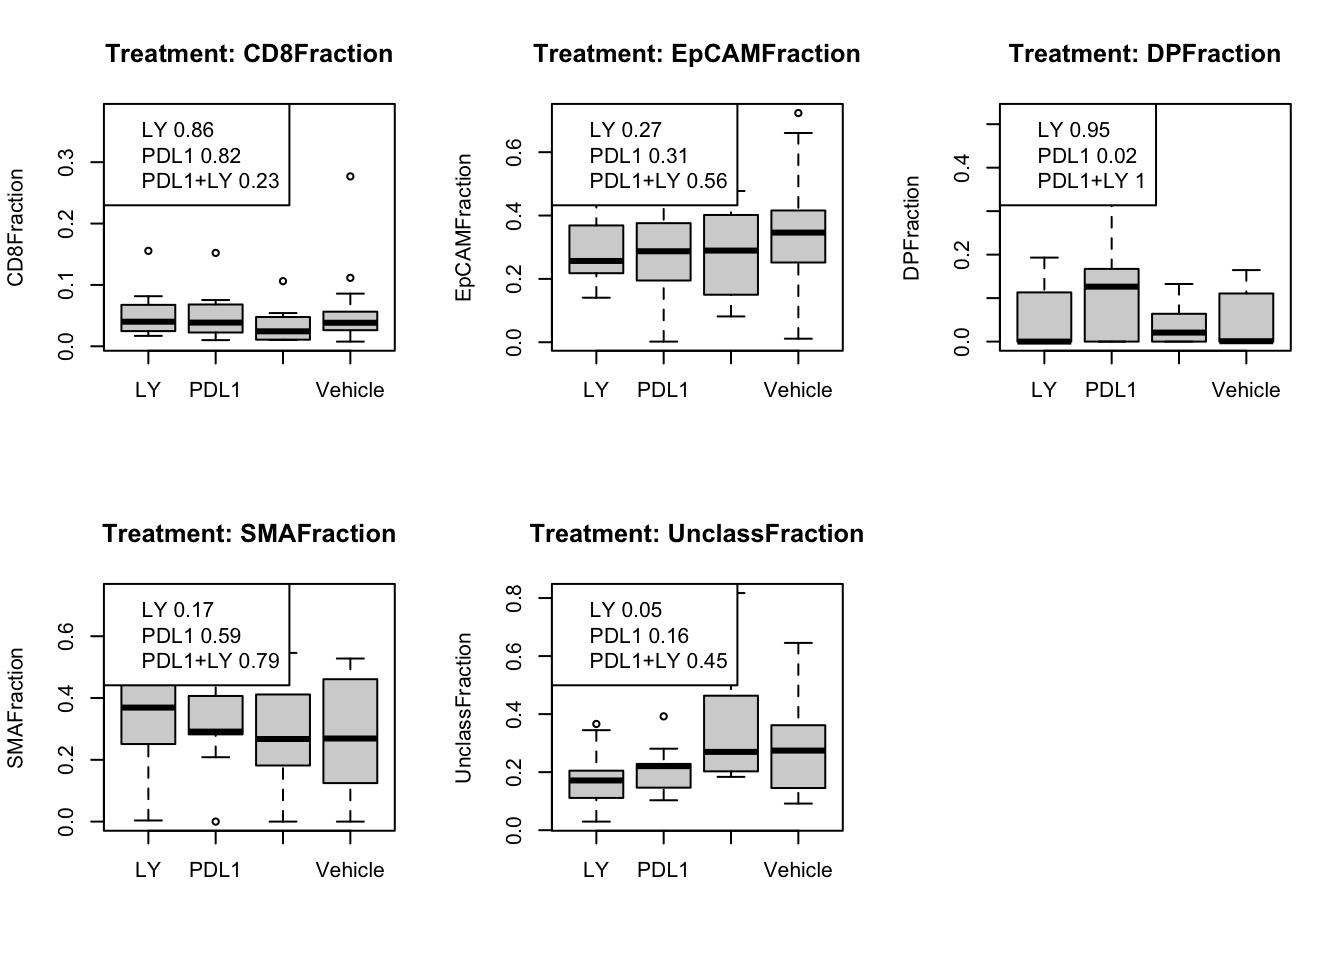
\includegraphics{RatDCIS-bookdown_files/figure-latex/unnamed-chunk-33-1.pdf}

\begin{verbatim}
## 
##  Pearson's product-moment correlation
## 
## data:  TareaSum and Tdiameter
## t = 1.6859, df = 54, p-value = 0.09759
## alternative hypothesis: true correlation is not equal to 0
## 95 percent confidence interval:
##  -0.04174574  0.45949702
## sample estimates:
##       cor 
## 0.2236089
\end{verbatim}

\hypertarget{correlations-between-different-subpopulations}{%
\section{Correlations between different subpopulations}\label{correlations-between-different-subpopulations}}

Look for correlates between different subpopulations: Naturally, we would expect a negative correlation since this should sum to 1. Below are heatmaps showing correlations between different cell types, and significant associations are linearly shown.

Note the following negative correlations:

\begin{itemize}
\tightlist
\item
  epcam and SMA
\item
  SMA+ and Unclass
\end{itemize}

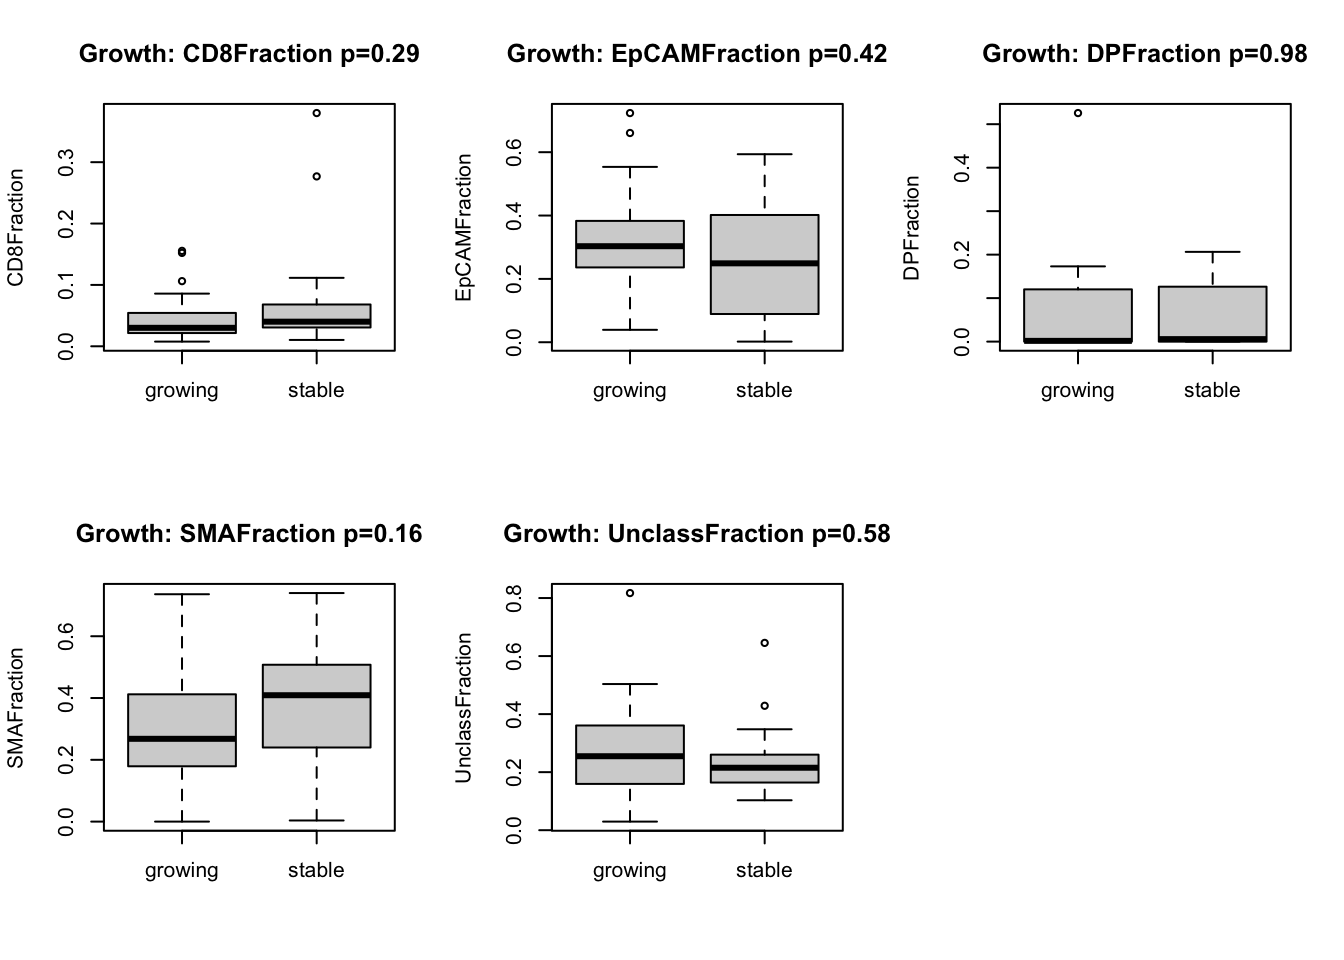
\includegraphics{RatDCIS-bookdown_files/figure-latex/unnamed-chunk-34-1.pdf} 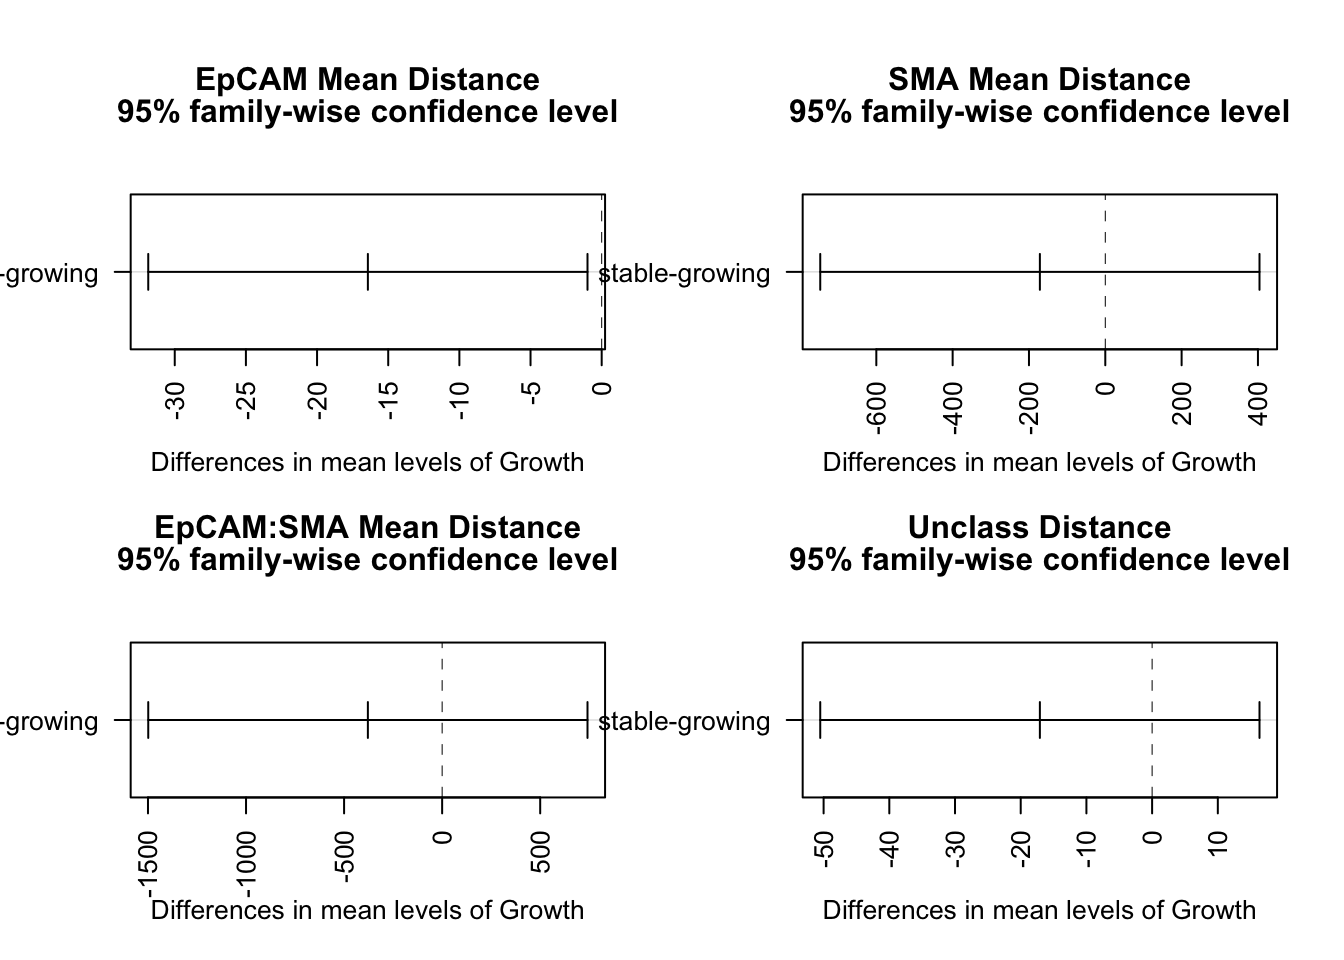
\includegraphics{RatDCIS-bookdown_files/figure-latex/unnamed-chunk-34-2.pdf}

\begin{verbatim}
##                   CD8      EpCAM EpCAM: SMA        SMA    Unclass
## CD8         1.0000000 -0.1780975 -0.1268947 -0.0344095 -0.1107879
## EpCAM      -0.1780975  1.0000000 -0.1595219 -0.5597908 -0.1898428
## EpCAM: SMA -0.1268947 -0.1595219  1.0000000 -0.2171477 -0.1783030
## SMA        -0.0344095 -0.5597908 -0.2171477  1.0000000 -0.4946850
## Unclass    -0.1107879 -0.1898428 -0.1783030 -0.4946850  1.0000000
\end{verbatim}

\begin{verbatim}
##           [,1]         [,2]      [,3]         [,4]        [,5]
## [1,] 0.0000000 1.891064e-01 0.3513624 8.012235e-01 0.416293560
## [2,] 0.1891064 0.000000e+00 0.2402481 7.272201e-06 0.161096722
## [3,] 0.3513624 2.402481e-01 0.0000000 1.079270e-01 0.188588161
## [4,] 0.8012235 7.272201e-06 0.1079270 0.000000e+00 0.000106427
## [5,] 0.4162936 1.610967e-01 0.1885882 1.064270e-04 0.000000000
\end{verbatim}

\hypertarget{associations-between-cd8-counts-with-other-clinical-variables}{%
\section{Associations between CD8 counts with other clinical variables}\label{associations-between-cd8-counts-with-other-clinical-variables}}

Below we assess whether any of the CD8-variables described in section 3.1 is associated with

\begin{itemize}
\tightlist
\item
  treatment
\item
  growth
\item
  spatial pattern
\end{itemize}

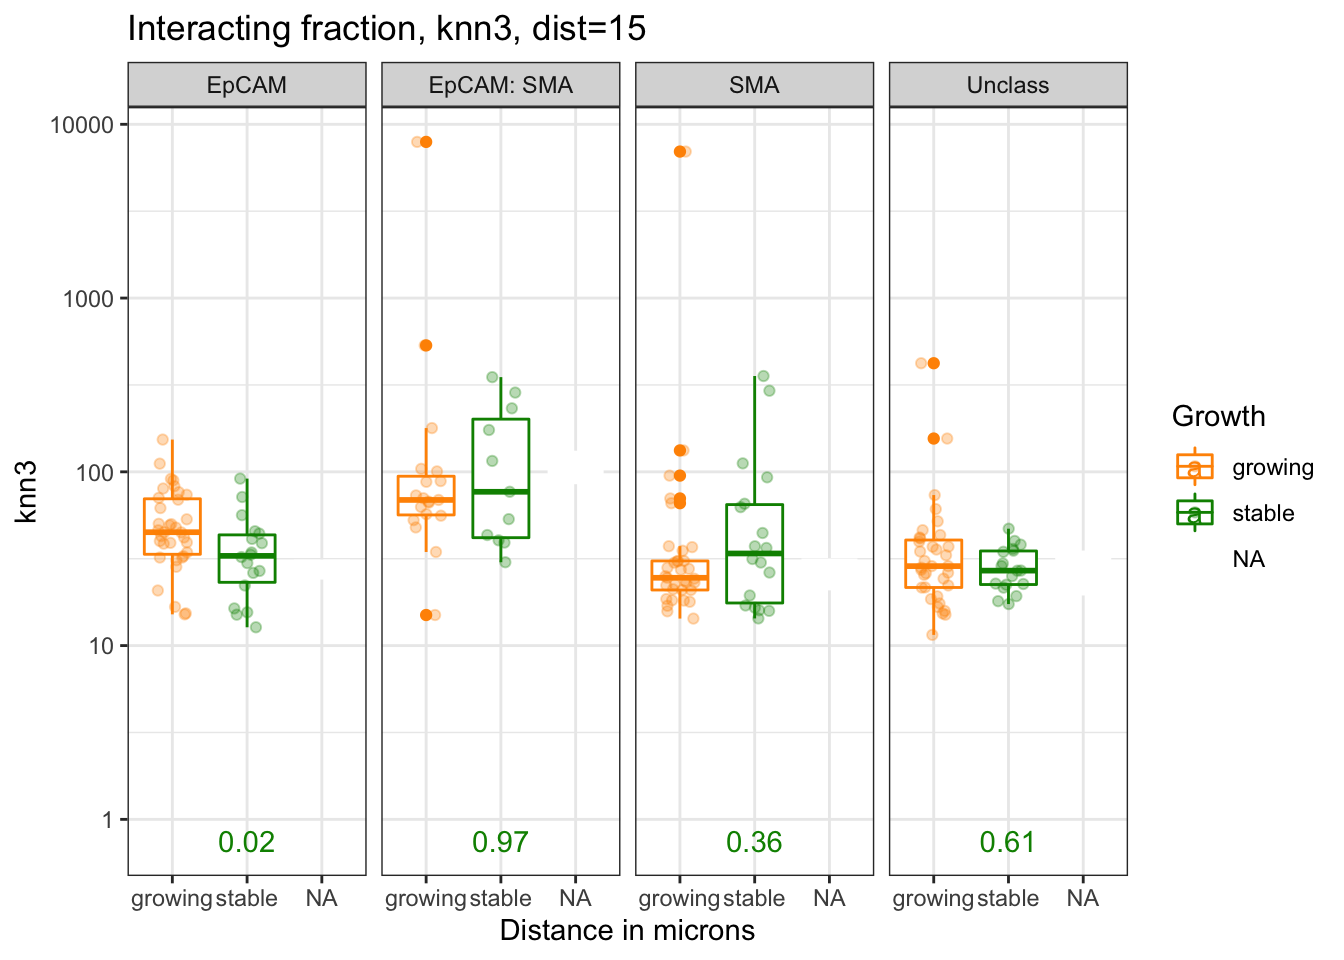
\includegraphics{RatDCIS-bookdown_files/figure-latex/unnamed-chunk-35-1.pdf}

Note that CD8 normalised by tumor size is associated with growth (but this could a reflection of the size of the tumor), and there is a borderline difference once normalised by epithelial content. In addition the CD8 total count is associated with pdl1+ly treatment.

Note that p=0.05 is designated by a value of 1.3

\hypertarget{spatial-statistics}{%
\chapter{Spatial statistics}\label{spatial-statistics}}

Below, we use three different metrics to compare spatial distributions:

\begin{itemize}
\tightlist
\item
  k-nearest neighbour distances
\item
  the interacting fraction
\item
  morisita-horn distances
\end{itemize}

These are compared to manual inspection of the result

\hypertarget{knn-distances}{%
\section{knn-Distances:}\label{knn-distances}}

The k-nearest neighbour distances looks at the average distance from a given cell type of class A to a cell type of class B. In this section, the reference class A is the CD8 T cell, and we will look at the mean distance to SMA, Epcam, double positive and unclassified cells in each image.

To account for potential fluctuations due to misclassified cells, or isolated single cells, k values of 1, 3, 5 will be used. I.e. for each cell, we will compute the mean distance from each Cd8Tcell to its 1, 3, and 5 nearest neighbours.

\hypertarget{comparison-to-manual-classification-treatment-growth}{%
\subsection{Comparison to manual classification, treatment, growth}\label{comparison-to-manual-classification-treatment-growth}}

Overall, we see that the differences in infiltrating vs restricted are similar. We see statistical differences (using anova followed by Tukey's test) between:

\begin{itemize}
\tightlist
\item
  epcam and SMA-epcam in both cases (higher distances to EpCAM on average)
\item
  SMA-Epcam to SMA (CD8s are closer to SMA+)
\item
  Unclass to Epcam-SMA (CD8s closer to unclass)
\end{itemize}

In the infiltrating case:

\begin{itemize}
\tightlist
\item
  Unclass to Epcam (CD8s closer to unclass, borderline significant)
\end{itemize}

In the restricted cases, we see:

\begin{itemize}
\tightlist
\item
  Unclass to SMA (higher distance to unclass in the restricted case)
\item
  SMA to epcam (CD8s are closer to the SMA)
\end{itemize}

This last result is consistent with what we expect for a CD8+ cell which is stroma-restricted.

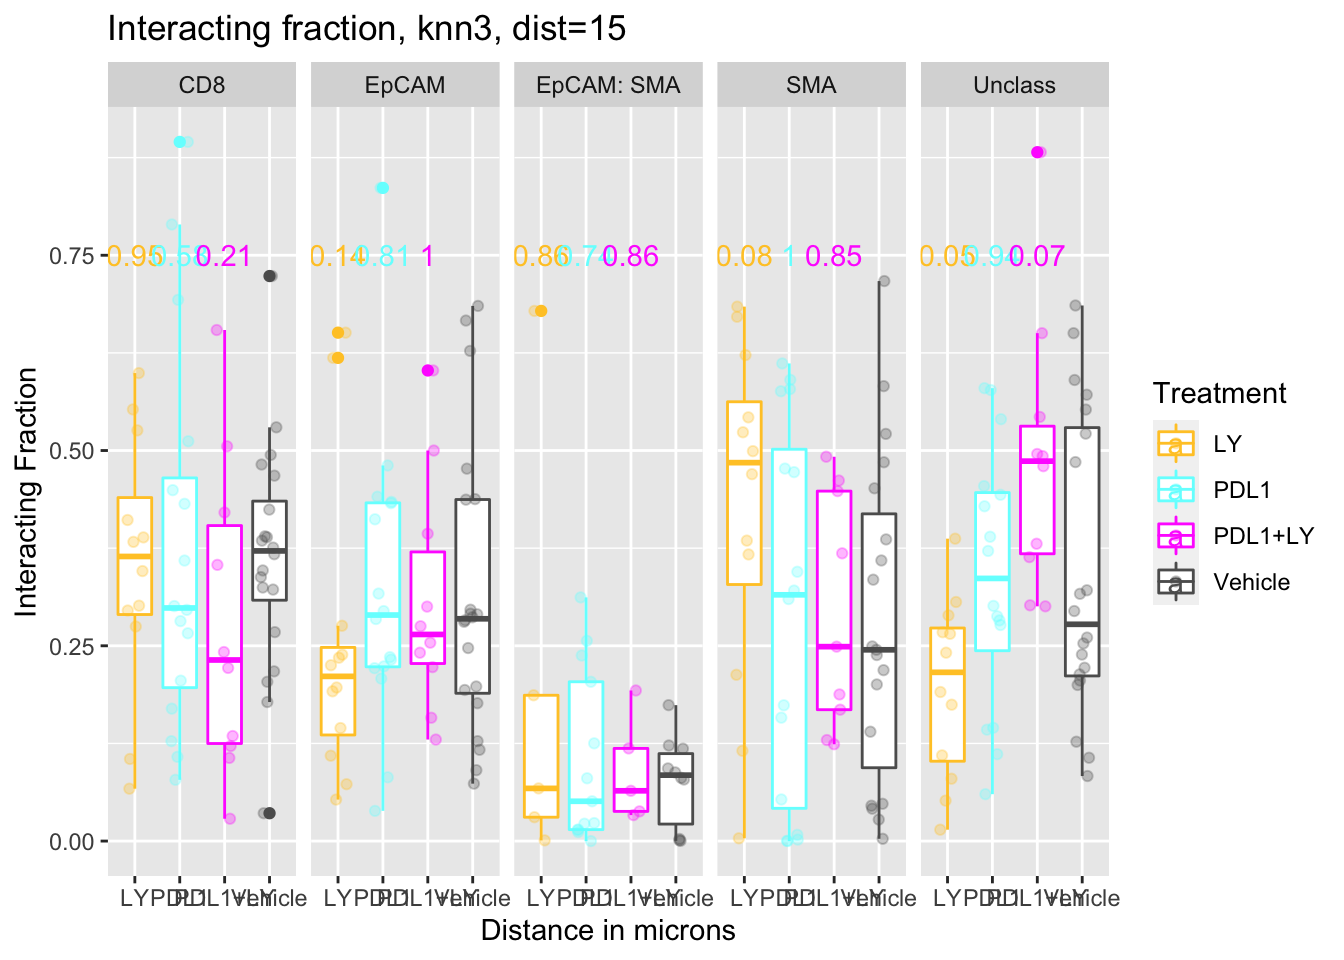
\includegraphics{RatDCIS-bookdown_files/figure-latex/unnamed-chunk-38-1.pdf} 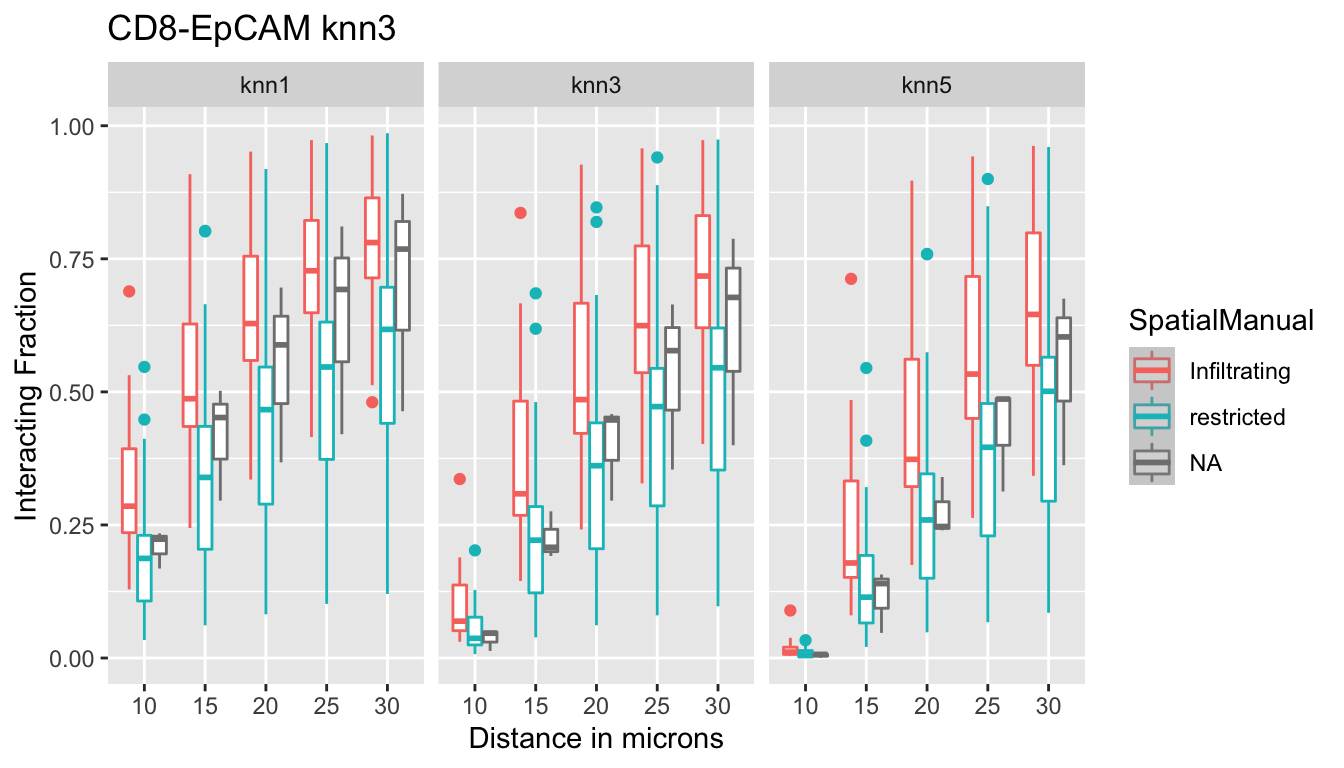
\includegraphics{RatDCIS-bookdown_files/figure-latex/unnamed-chunk-38-2.pdf}

\hypertarget{associations-with-outcome}{%
\subsection{Associations with outcome}\label{associations-with-outcome}}

We can also see if there is an association between these distances with growth and treatment

Treatment:

\begin{itemize}
\tightlist
\item
  CD8 cells in PDL1 sample are further away to SMA+ cells and EpCAM+ (compared to vehicle or double agent)
\item
  CD8 cells in LY treated samples are further away from unclassified cells (compared to any of the other treatments)
\end{itemize}

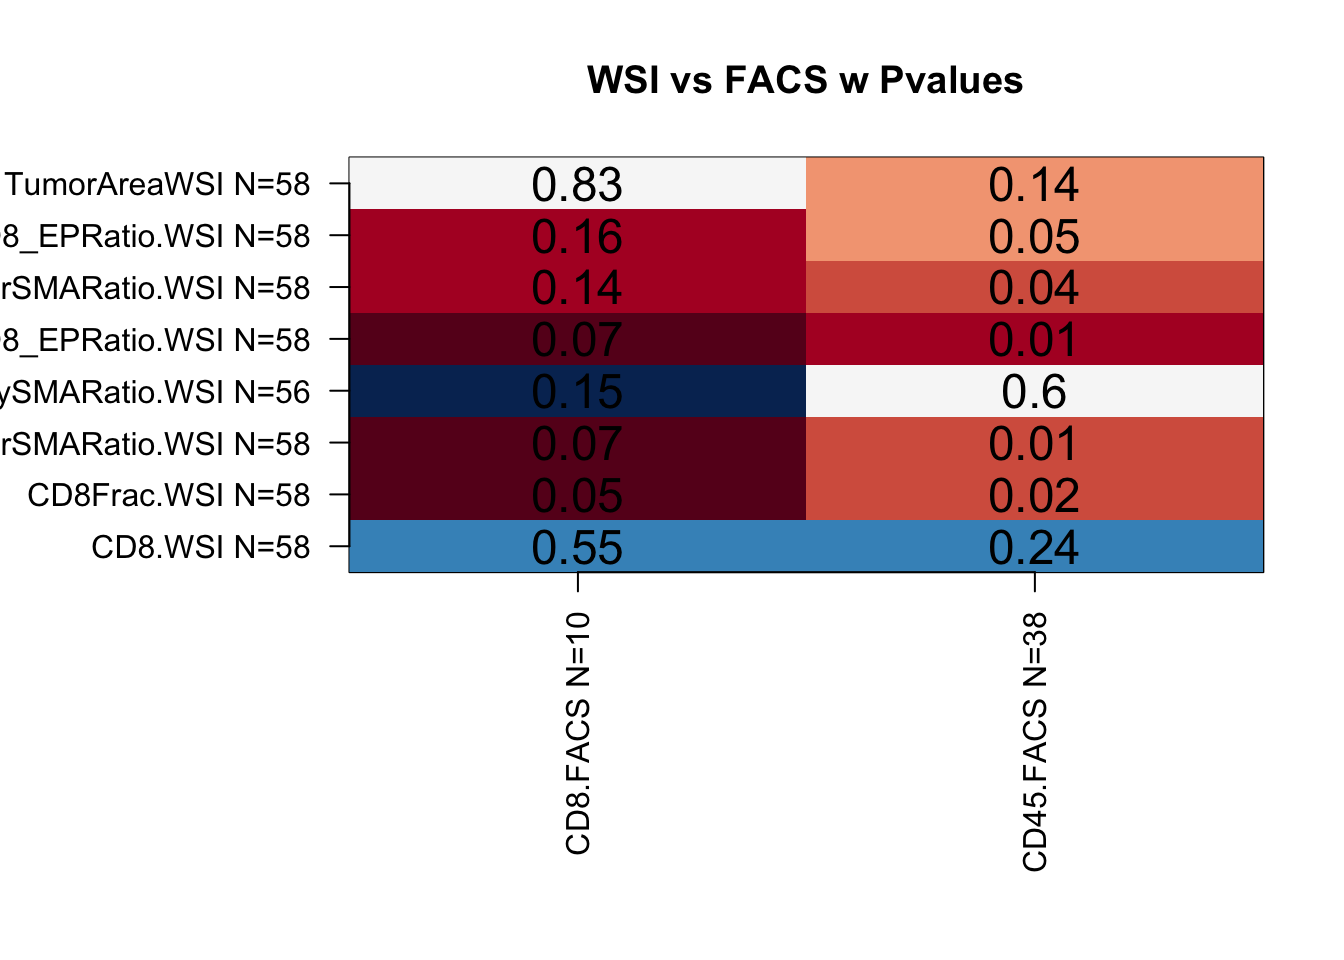
\includegraphics{RatDCIS-bookdown_files/figure-latex/unnamed-chunk-39-1.pdf} 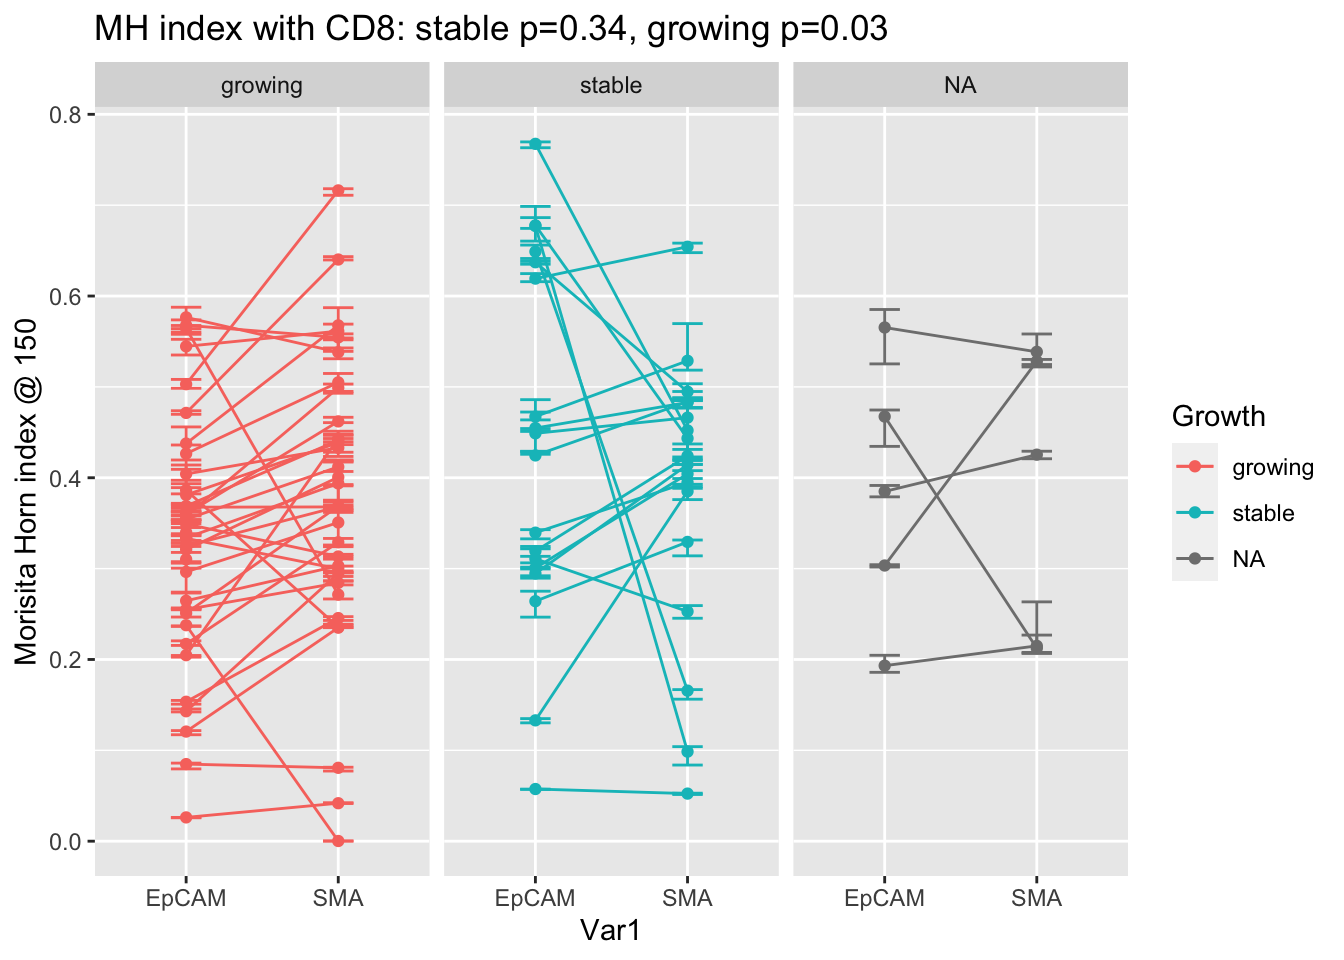
\includegraphics{RatDCIS-bookdown_files/figure-latex/unnamed-chunk-39-2.pdf}

\hypertarget{growth}{%
\subsection{Growth}\label{growth}}

All 95\% confidence lines cross 0, but it appears that stable cases have a closer unclass-CD8 interaction distance compared to growing.

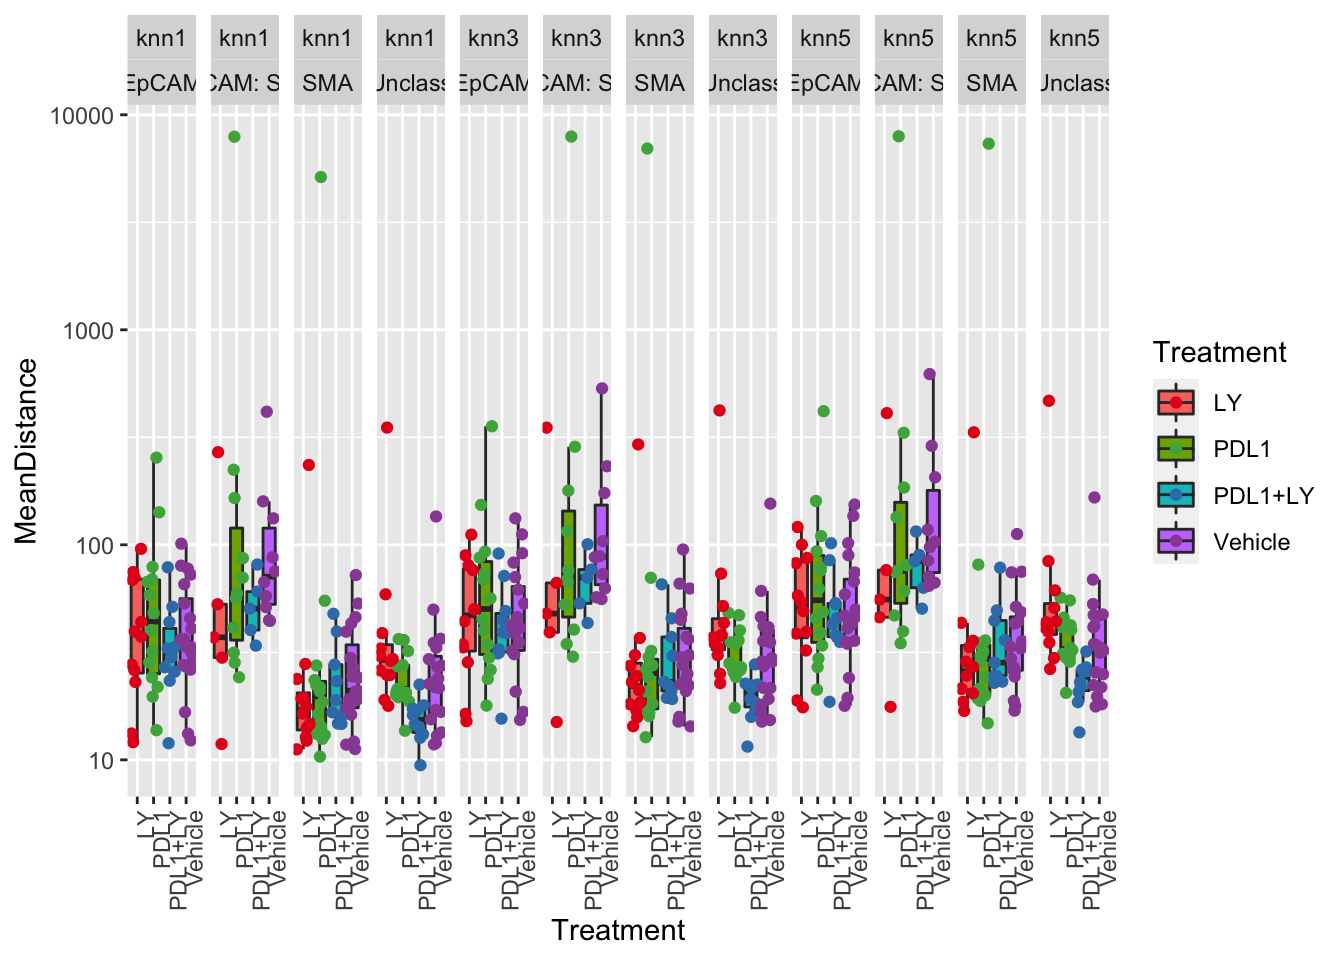
\includegraphics{RatDCIS-bookdown_files/figure-latex/unnamed-chunk-40-1.pdf} 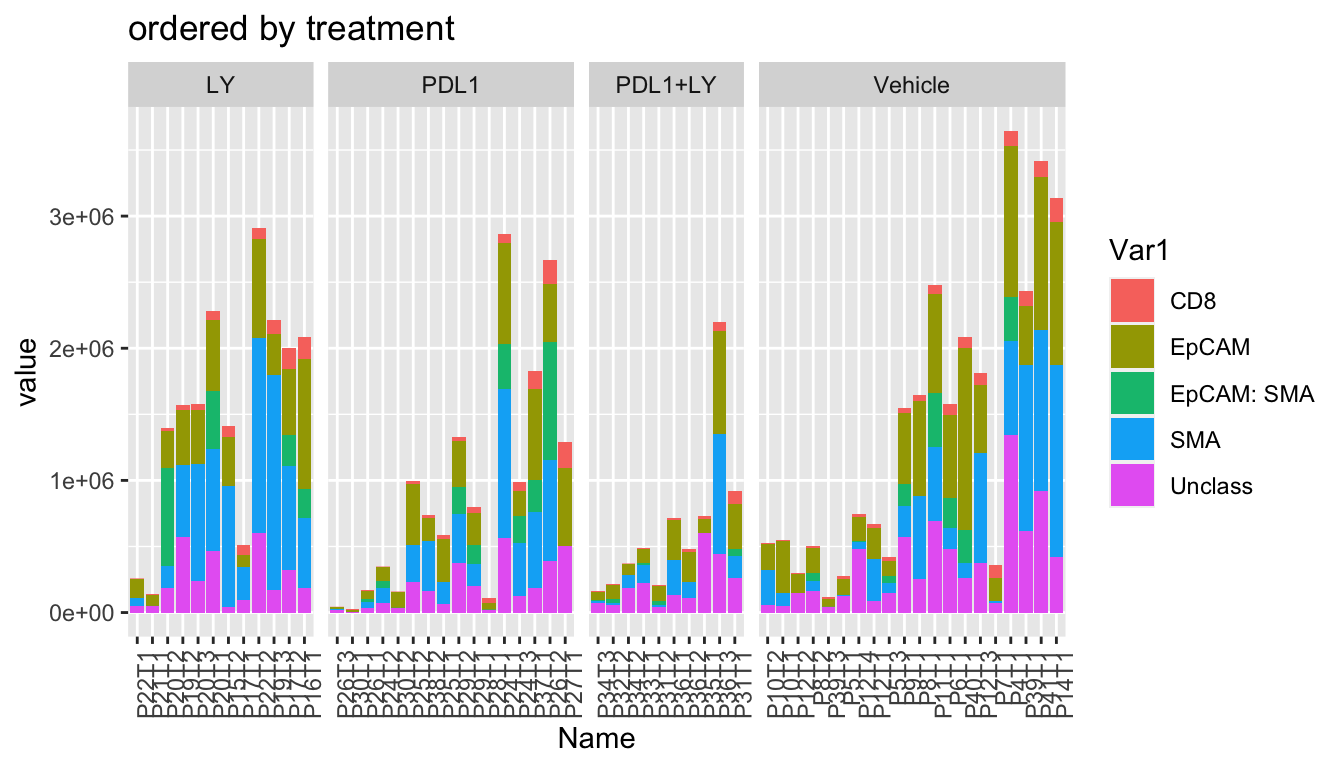
\includegraphics{RatDCIS-bookdown_files/figure-latex/unnamed-chunk-40-2.pdf}

Based on the above distributions, knn1, knn3, and knn5 analyses give similar results. In the following section, we will make comparisons using knn3 results.

\hypertarget{association-between-distance-and-content}{%
\subsection{Association between distance and content}\label{association-between-distance-and-content}}

The spatial differences could be influenced by CD8 content. Here, we test if the distances from CD8Tcells to celltype B could be influenced by this.

We see that there is a correlation between CD8 fraction and the SMA proportion (both SMA and double positive).
But we don't see an association with epcam+ cells or unclassified stromal cells

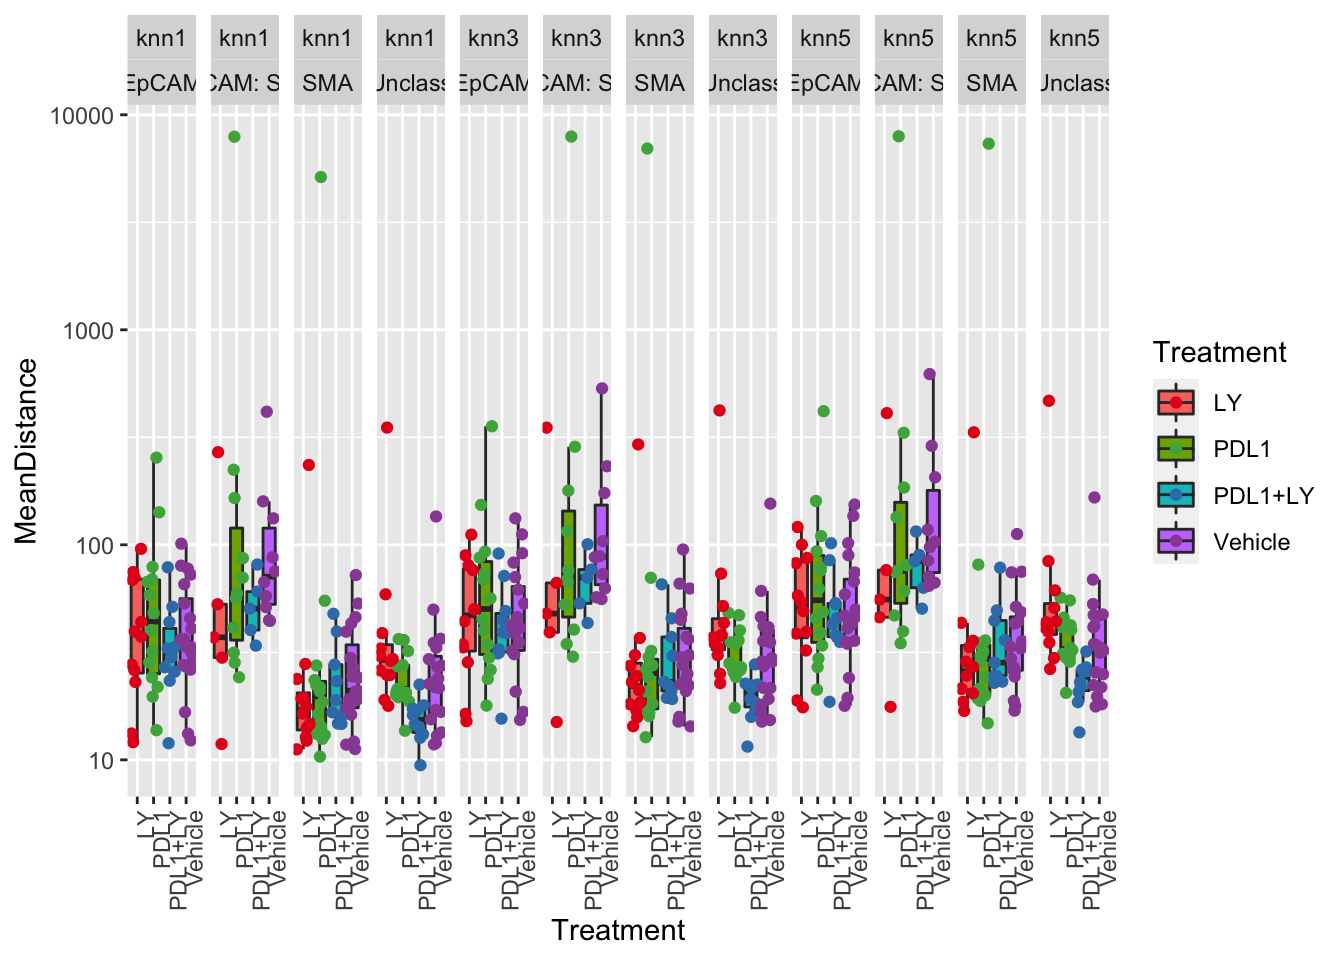
\includegraphics{RatDCIS-bookdown_files/figure-latex/unnamed-chunk-41-1.pdf}

CD8-Epcam distances are looked at in greater detail below. Here, we look at whether there is an association with CD8 fraction in a growing and stable tumors.

In growing or spatially restricted tumors, there is an association between the CD8-epcam distances with the CD8 fraction, but not in infiltrating or stable tumours.

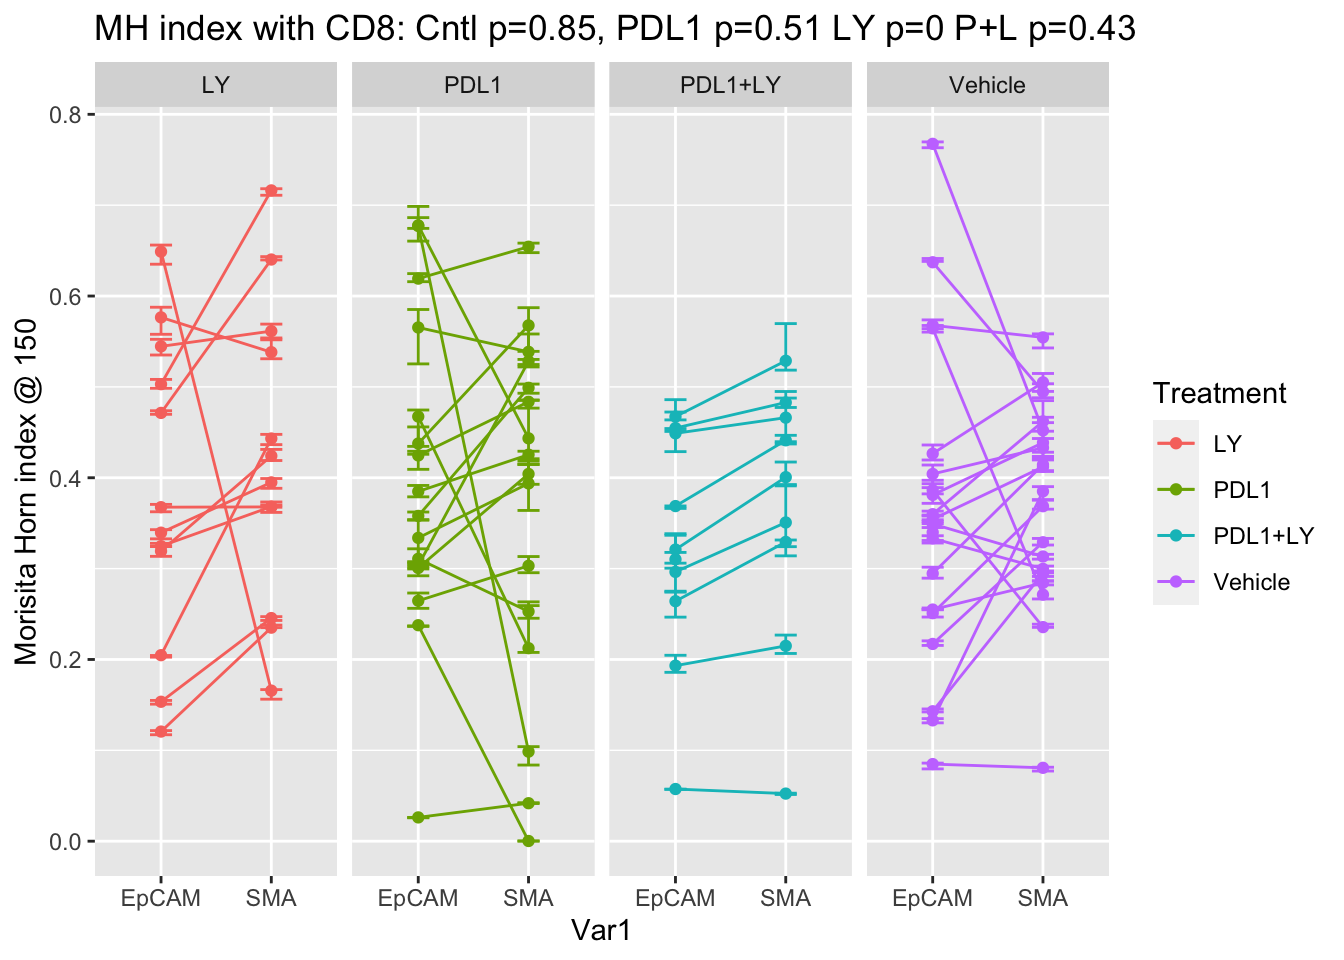
\includegraphics{RatDCIS-bookdown_files/figure-latex/unnamed-chunk-42-1.pdf}

Do any of the below metrics correlate with manual scoring:

\begin{itemize}
\tightlist
\item
  We can assess the distances from CD8 cells which come automatically:

  \begin{itemize}
  \tightlist
  \item
    Ep-distance
  \item
    SMA distance
  \item
    Ep:SMA distance
  \item
    SMA distance.
  \end{itemize}
\item
  EpMIN: distance to any Epcam expressing cell (includes EP+SMA+)
\item
  Ratios between Epcam and SMA: There are different values depending on whether the double positive fraction is used or not

  \begin{itemize}
  \tightlist
  \item
    (Ratio 1): Ep/any SMA
  \item
    (Ratio 2): EP/SMA
  \item
    (Ratio 3): Any Ep / Any SMA
  \item
    (Ratio 4): Any Ep/ SMA
  \end{itemize}
\end{itemize}

Whilst the manual scorings associate strongly with CD8-EPcam distances, there is no association with any other cell type.

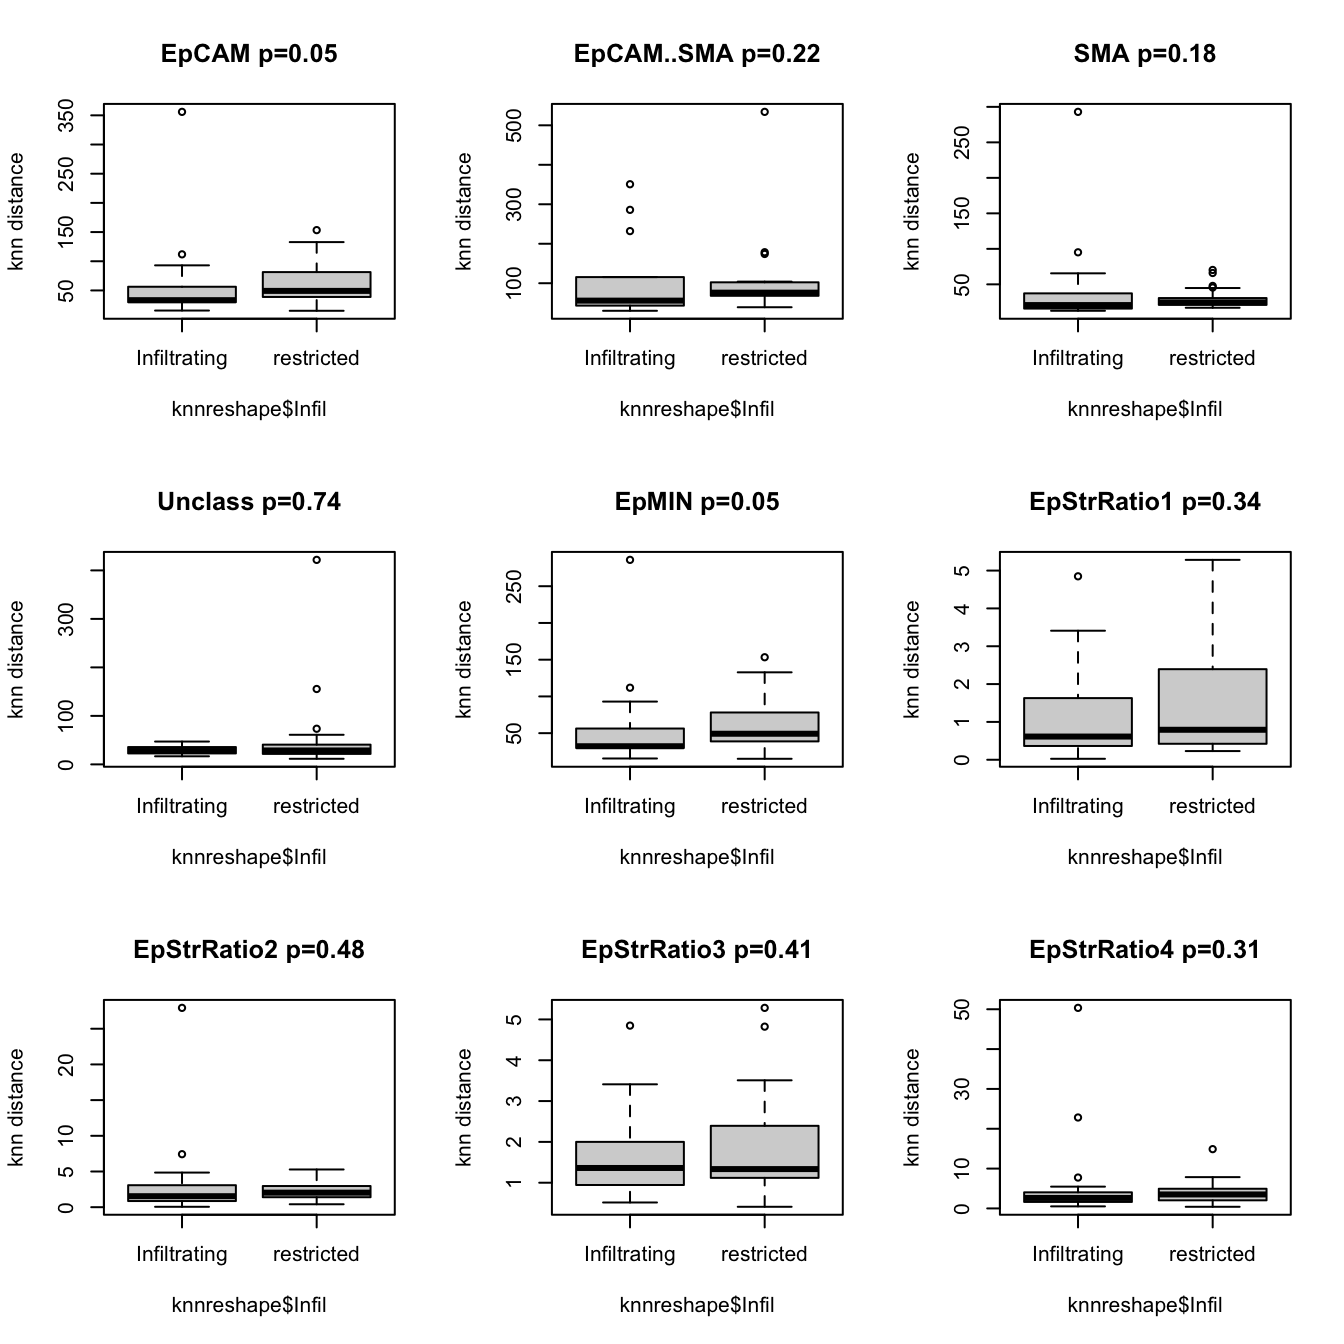
\includegraphics{RatDCIS-bookdown_files/figure-latex/unnamed-chunk-43-1.pdf}

\hypertarget{the-interacting-fraction}{%
\section{The interacting fraction}\label{the-interacting-fraction}}

The interacting fraction uses the knn-distances and determines the proportion of CD8 cells which are within a proximity of r um from celltype B.

\hypertarget{comparison-to-manual-select-optimal-r}{%
\subsection{Comparison to manual \& select optimal r}\label{comparison-to-manual-select-optimal-r}}

Below are plots of the proportion of CD8 cells within an ``interacting distance'' as we increase r. This looks at both the interacting fraction of CD8 cells with Epcam+ and SMA+ cells. Lines are color coded according to the manual spatial-infiltration annotation.

We notice from the line plots for each single sample that the restricted samples generally have low interacting fractins with EpCAM and SMA compared to the infiltrating samples. In addition, there is a statistical difference in EpCAM measurements compared to SMA.

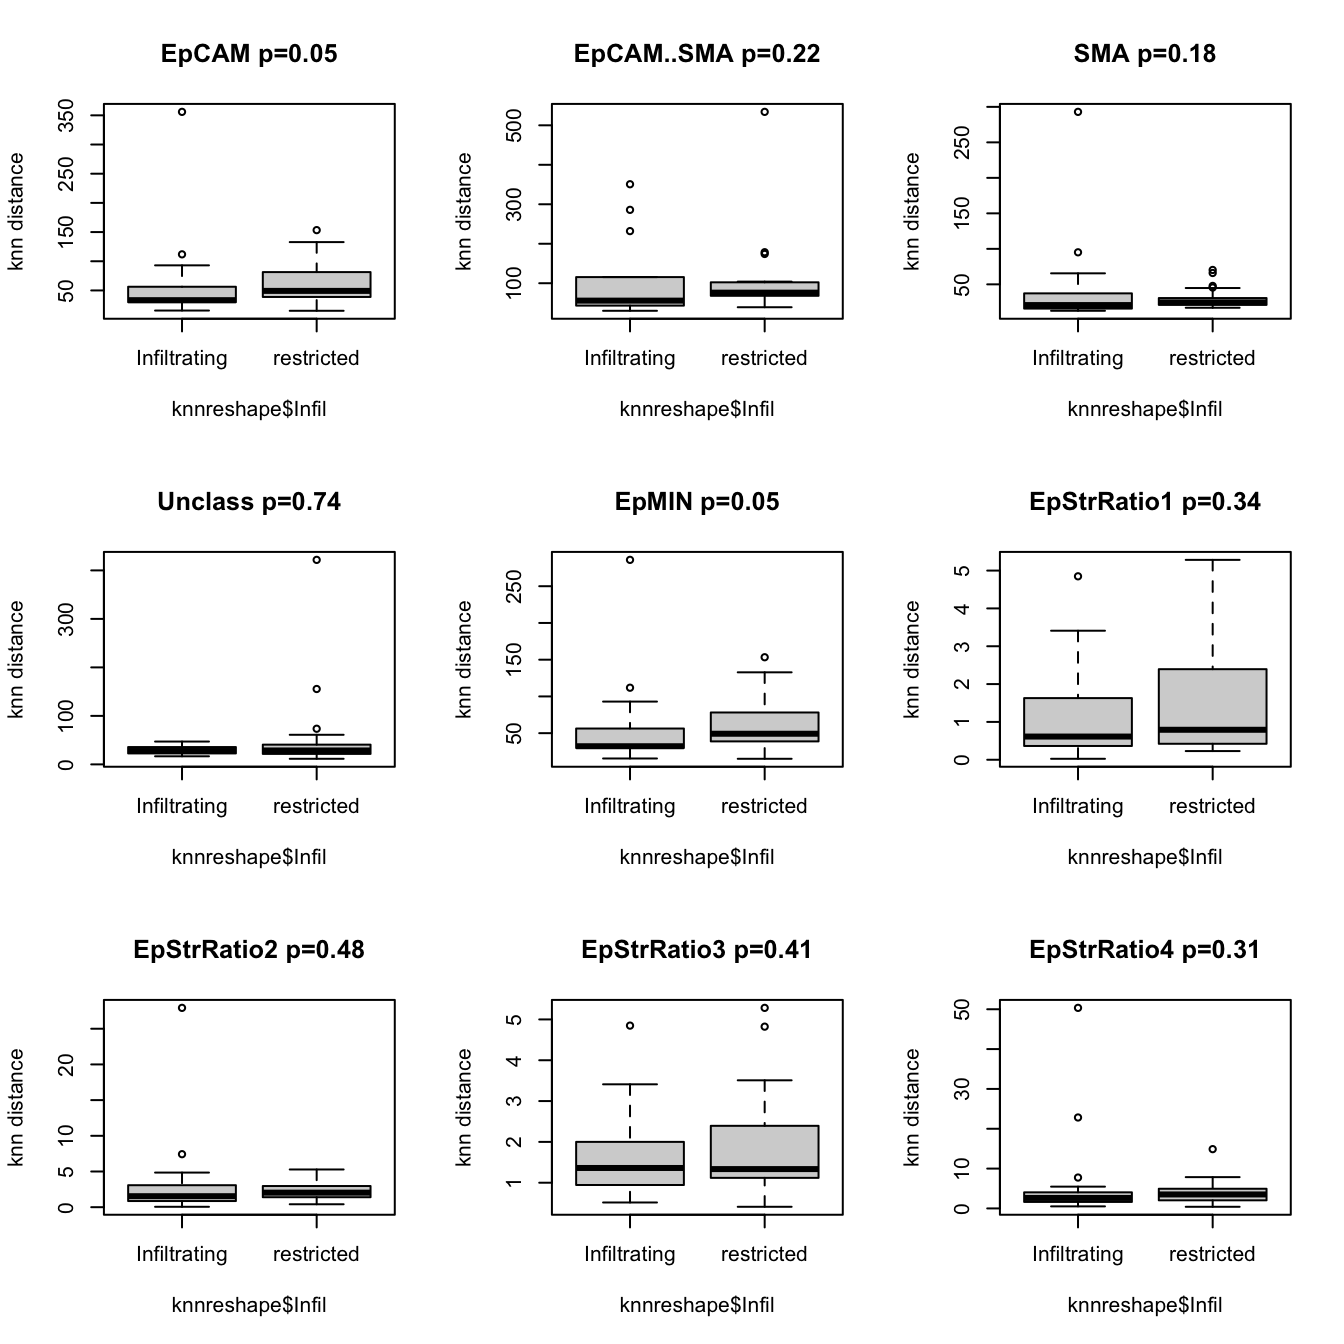
\includegraphics{RatDCIS-bookdown_files/figure-latex/unnamed-chunk-44-1.pdf} 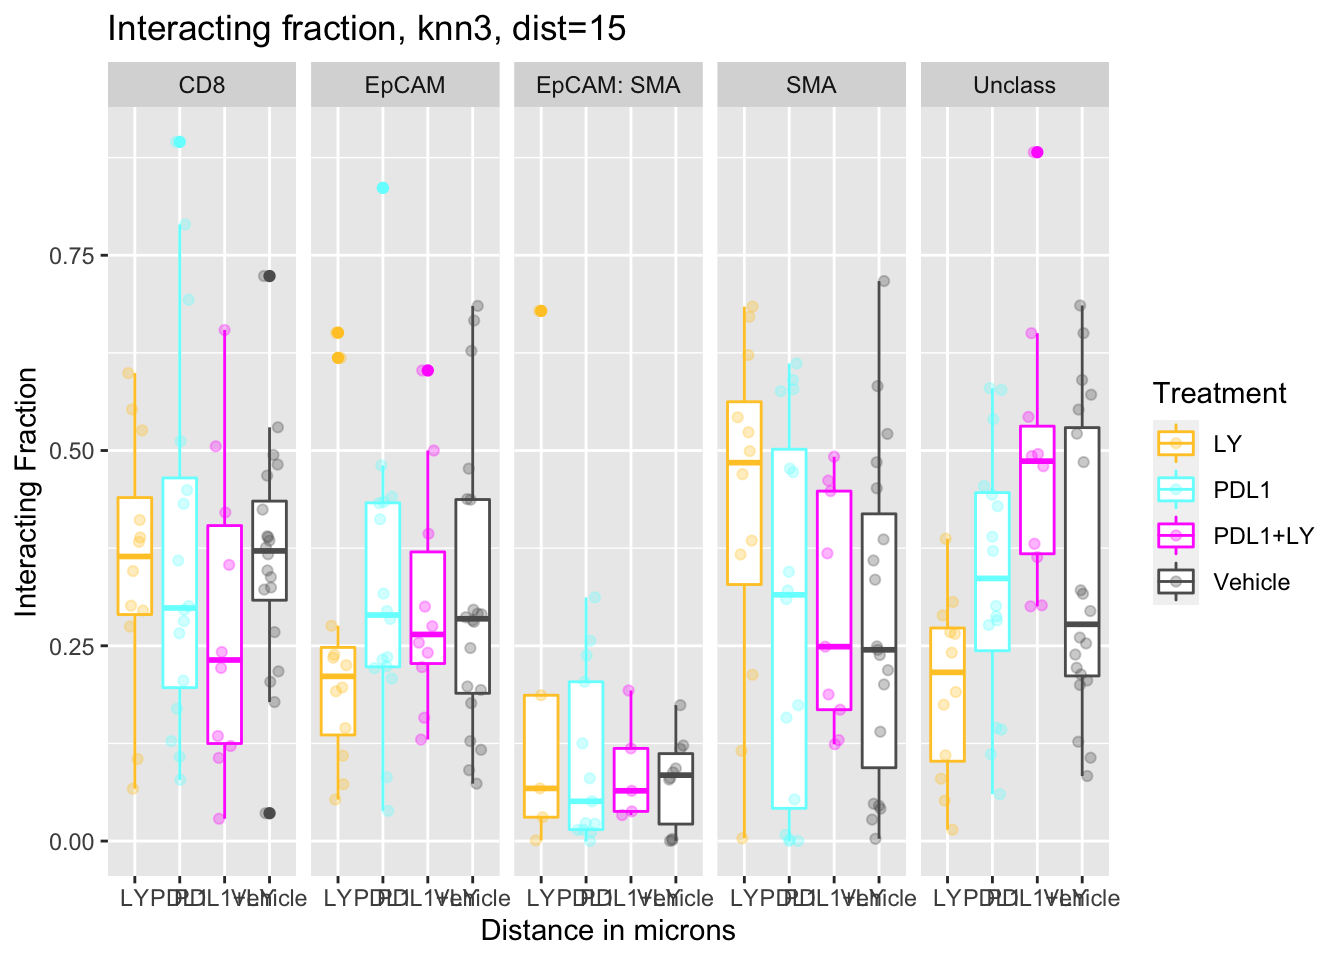
\includegraphics{RatDCIS-bookdown_files/figure-latex/unnamed-chunk-44-2.pdf} 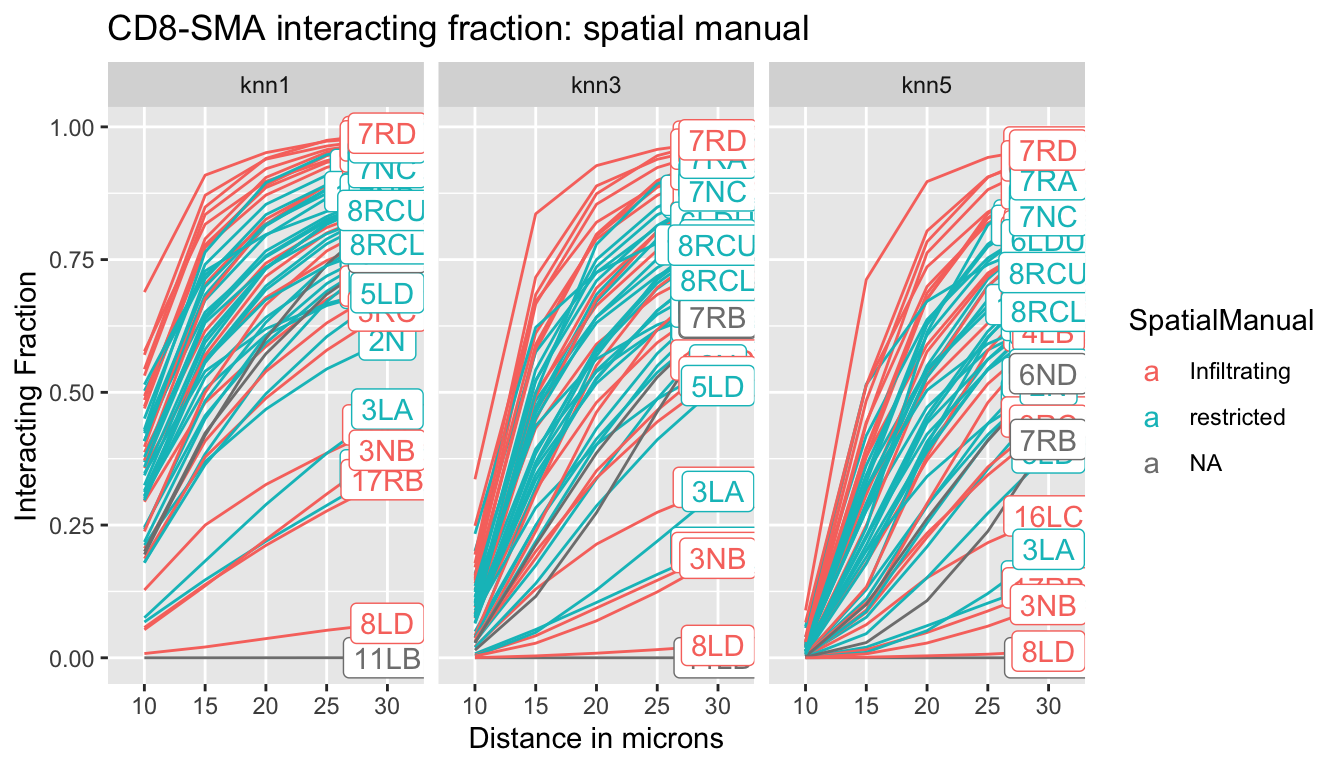
\includegraphics{RatDCIS-bookdown_files/figure-latex/unnamed-chunk-44-3.pdf} 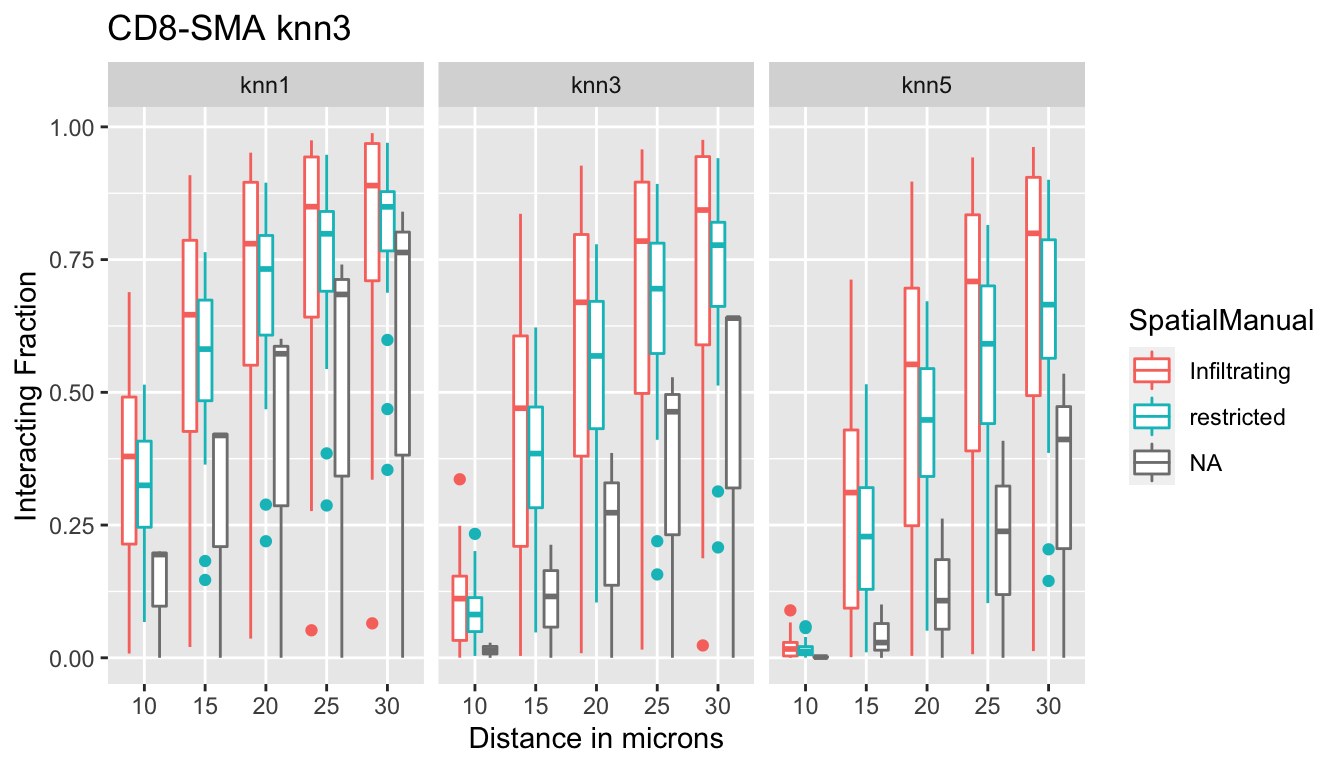
\includegraphics{RatDCIS-bookdown_files/figure-latex/unnamed-chunk-44-4.pdf}

Using the boxplots as a guide, we can determine optimal ``interacting distances'' at which to perform downstream analysis. The best separation between restricted and infiltrating for EpCAM appears at:

\begin{itemize}
\tightlist
\item
  1-nn: 10-15 um
\item
  3-nn: 15 um
\item
  5-nn: 20 um
\end{itemize}

The interacting fraction does not distinguish SMA fractions (all restricted boxplots overlap with the infiltrating boxplots)

The following plots use 3NN analysis with an interacting distance of 15um. We can firstly check if there is an association between different ``interacting fraction'' types and manual scoring, similar to what was performed for knn-analysis. Only CD8-EpCAM interacting distances is associated with manual scoring. All other metrics are not significant.

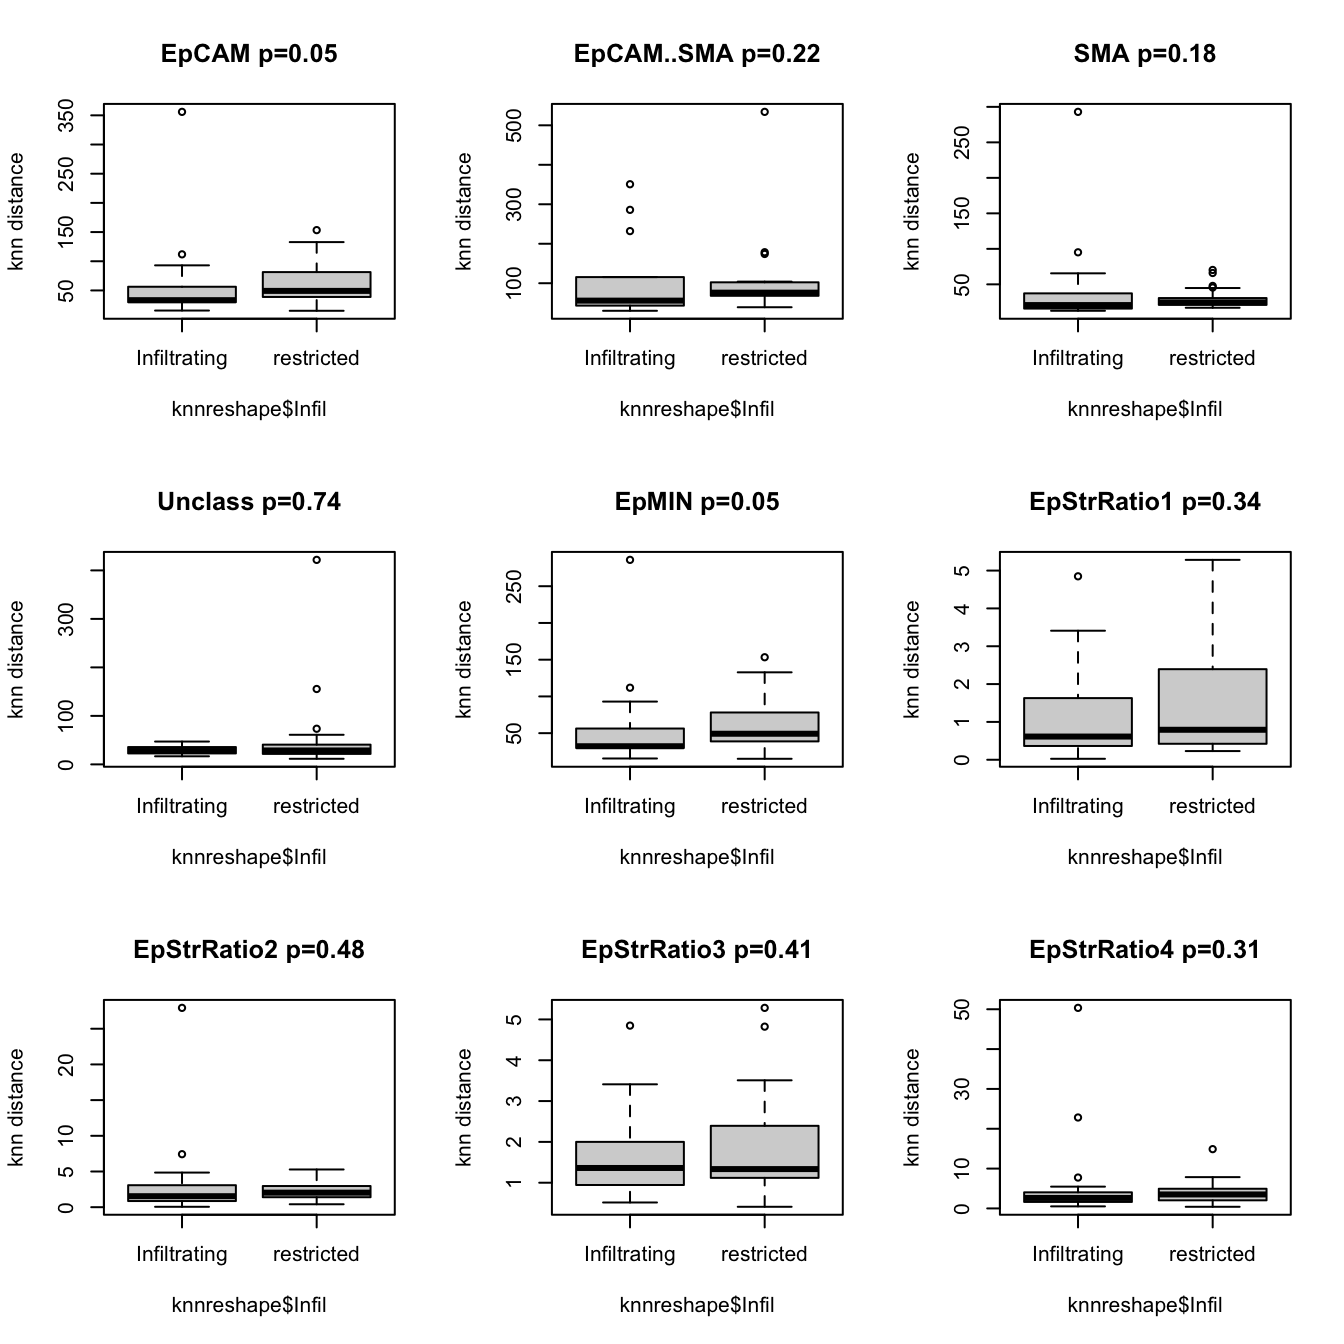
\includegraphics{RatDCIS-bookdown_files/figure-latex/unnamed-chunk-45-1.pdf}

Again, association between CD8 content and interacting fraction was observed ONLY in the growing samples or restricted cases.

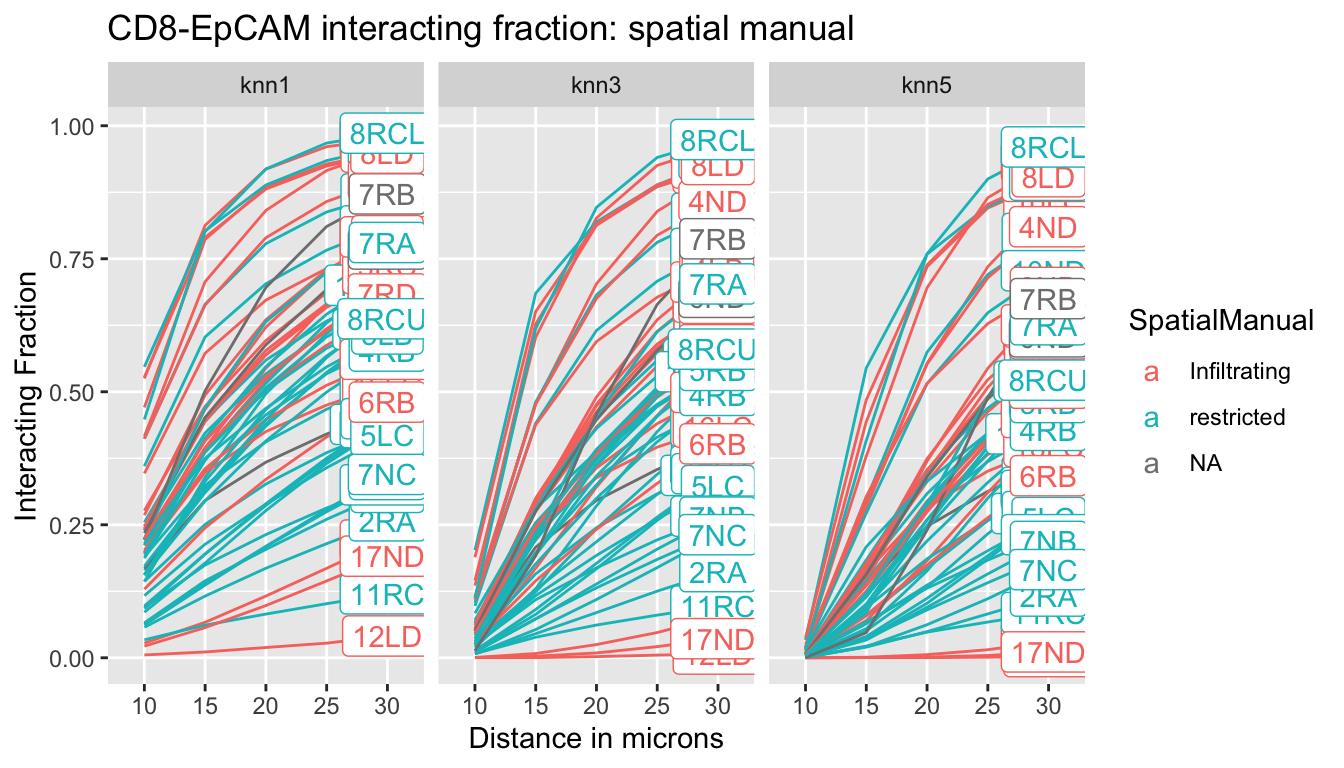
\includegraphics{RatDCIS-bookdown_files/figure-latex/unnamed-chunk-46-1.pdf}

\hypertarget{growth-1}{%
\subsection{Growth}\label{growth-1}}

Here, we check if there is an association between the spatial pattern and tumor growth.

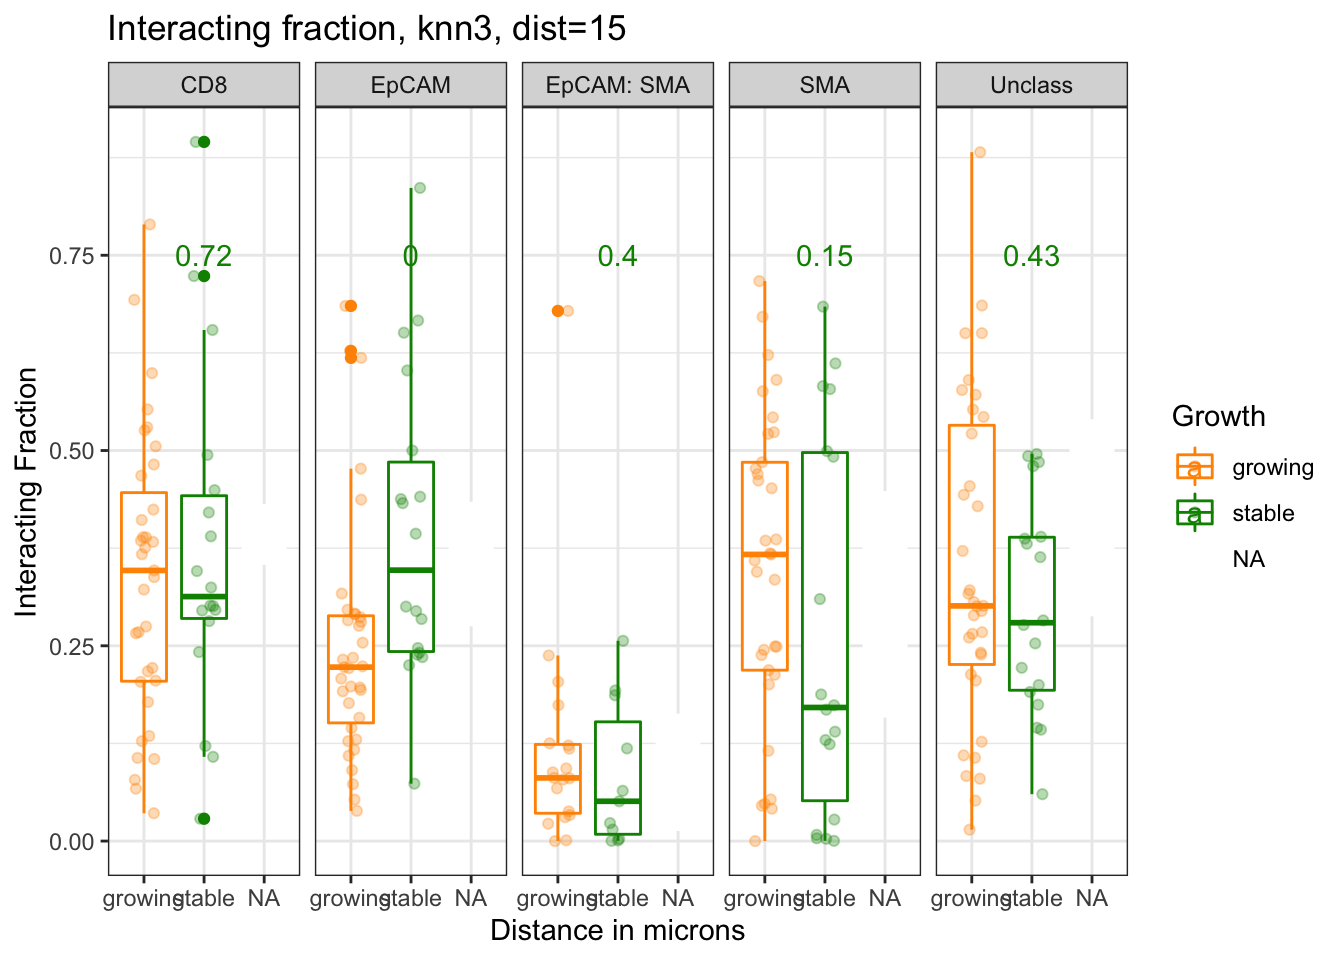
\includegraphics{RatDCIS-bookdown_files/figure-latex/if-growth-1.pdf}

None of the above metrics associate with growth. (P value by wilcox test shown)

\hypertarget{treatment}{%
\subsection{Treatment}\label{treatment}}

Similarly, compare the distances with treatment:

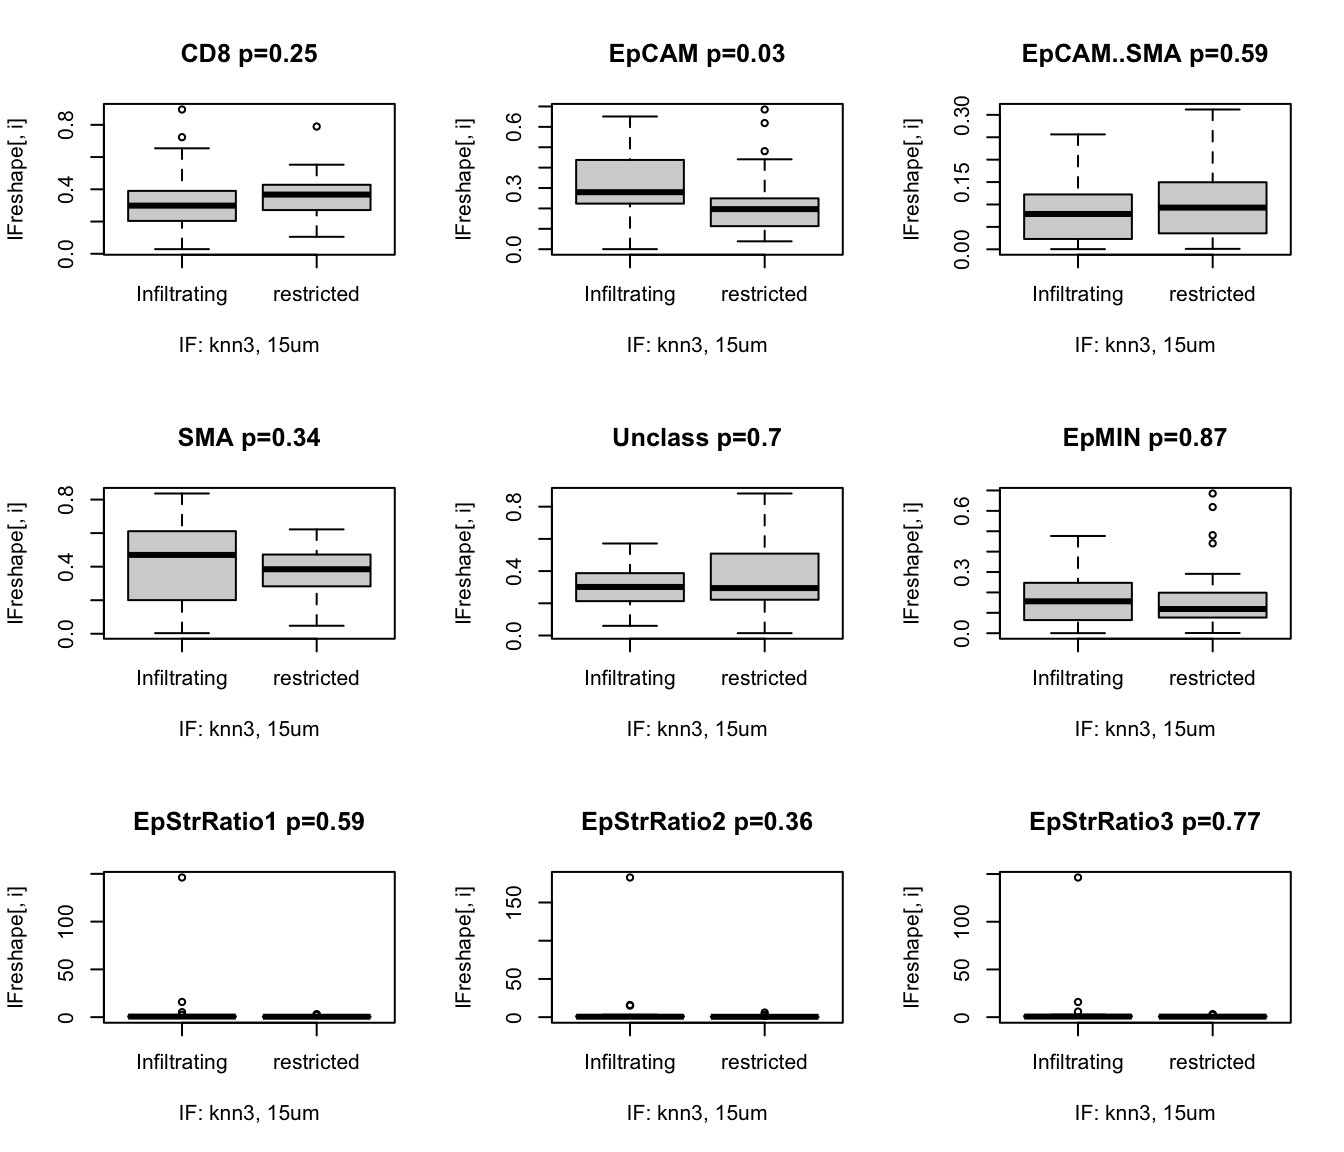
\includegraphics{RatDCIS-bookdown_files/figure-latex/unnamed-chunk-47-1.pdf} 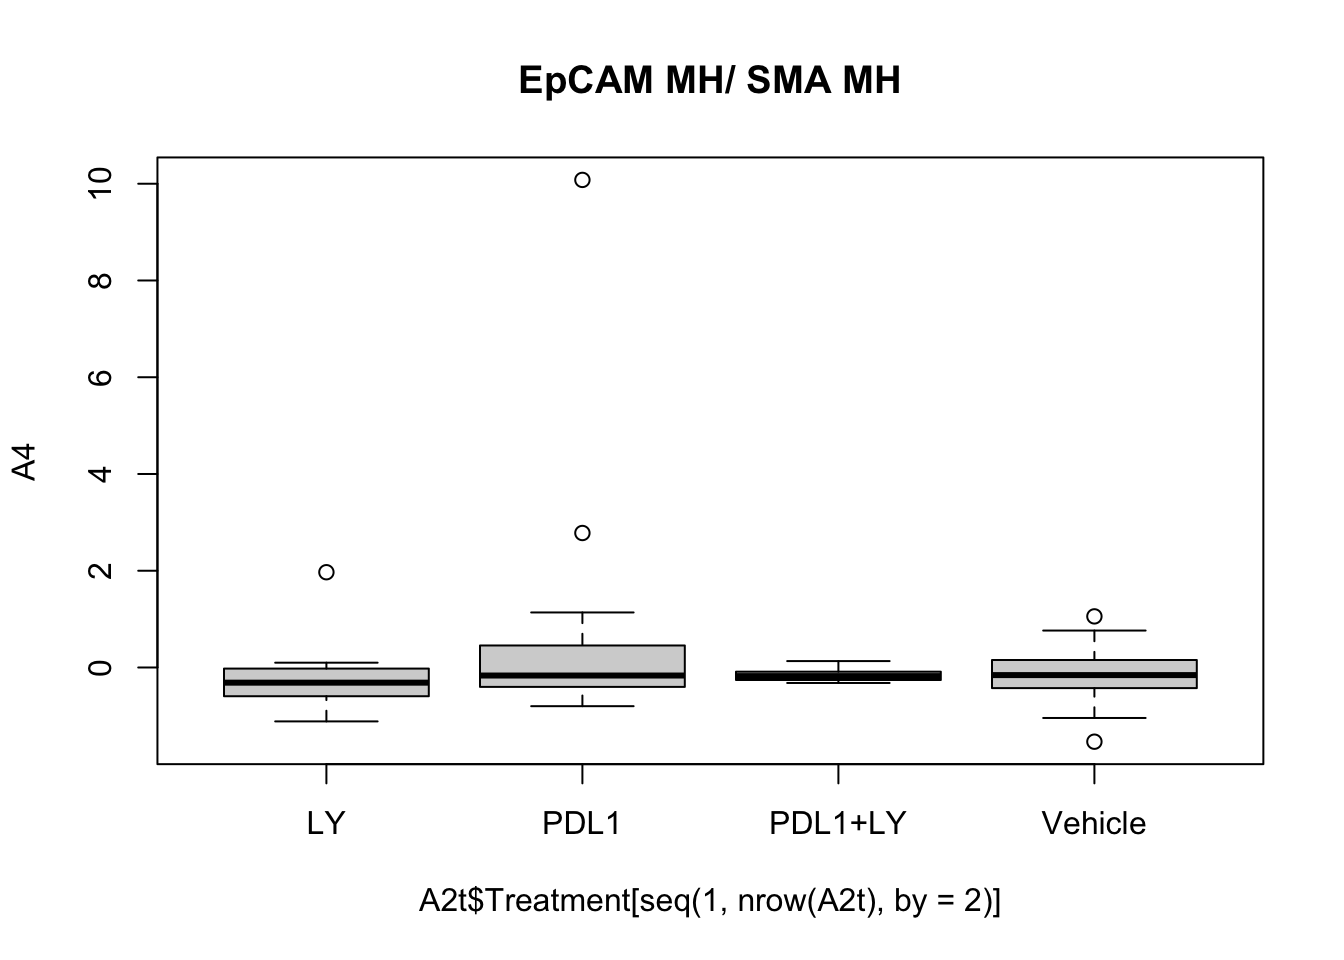
\includegraphics{RatDCIS-bookdown_files/figure-latex/unnamed-chunk-47-2.pdf}

There appears to be a difference in CD8-unclass interactions in LY treated samples (LY, PDL1+LY), but not in the other cases

\hypertarget{m-h-distances}{%
\section{M-H distances}\label{m-h-distances}}

The M-H distance (or Morisita Horn index) can be considered as a correlation coefficient in spatial distribution between cell type A and cell type B. To calculate this metric, the whole slide image is divided into grids of size 50 to 500um. Within each grid, the total number of cells A and B are determined.

The M-H index is thus determined as:

\[ \frac{2\sum_{i=1}^n a_ib_i}{(D_a+D_b)AB} \]
where \(a_i\) and \(b_i\) are the number of cells in grid \(i\), \[A\] and \[B\] the total number of cells, and \[D_x\] is the Simpson's index.

\hypertarget{comparison-to-manual-scoring}{%
\subsection{Comparison to Manual Scoring}\label{comparison-to-manual-scoring}}

Similar to the interacting fraction, we plot the MH index for increasing values of gridsize to determine an optimal metric to compare spatial patterns. Ideally, we would pick a metric has the following properties:

\begin{itemize}
\tightlist
\item
  good separation of the different values
\item
  a reasonable number of cells within each grid (avoid too small grids which give counts of 0)
\item
  avoid plateauing of MH values because the grid size is too large
\end{itemize}

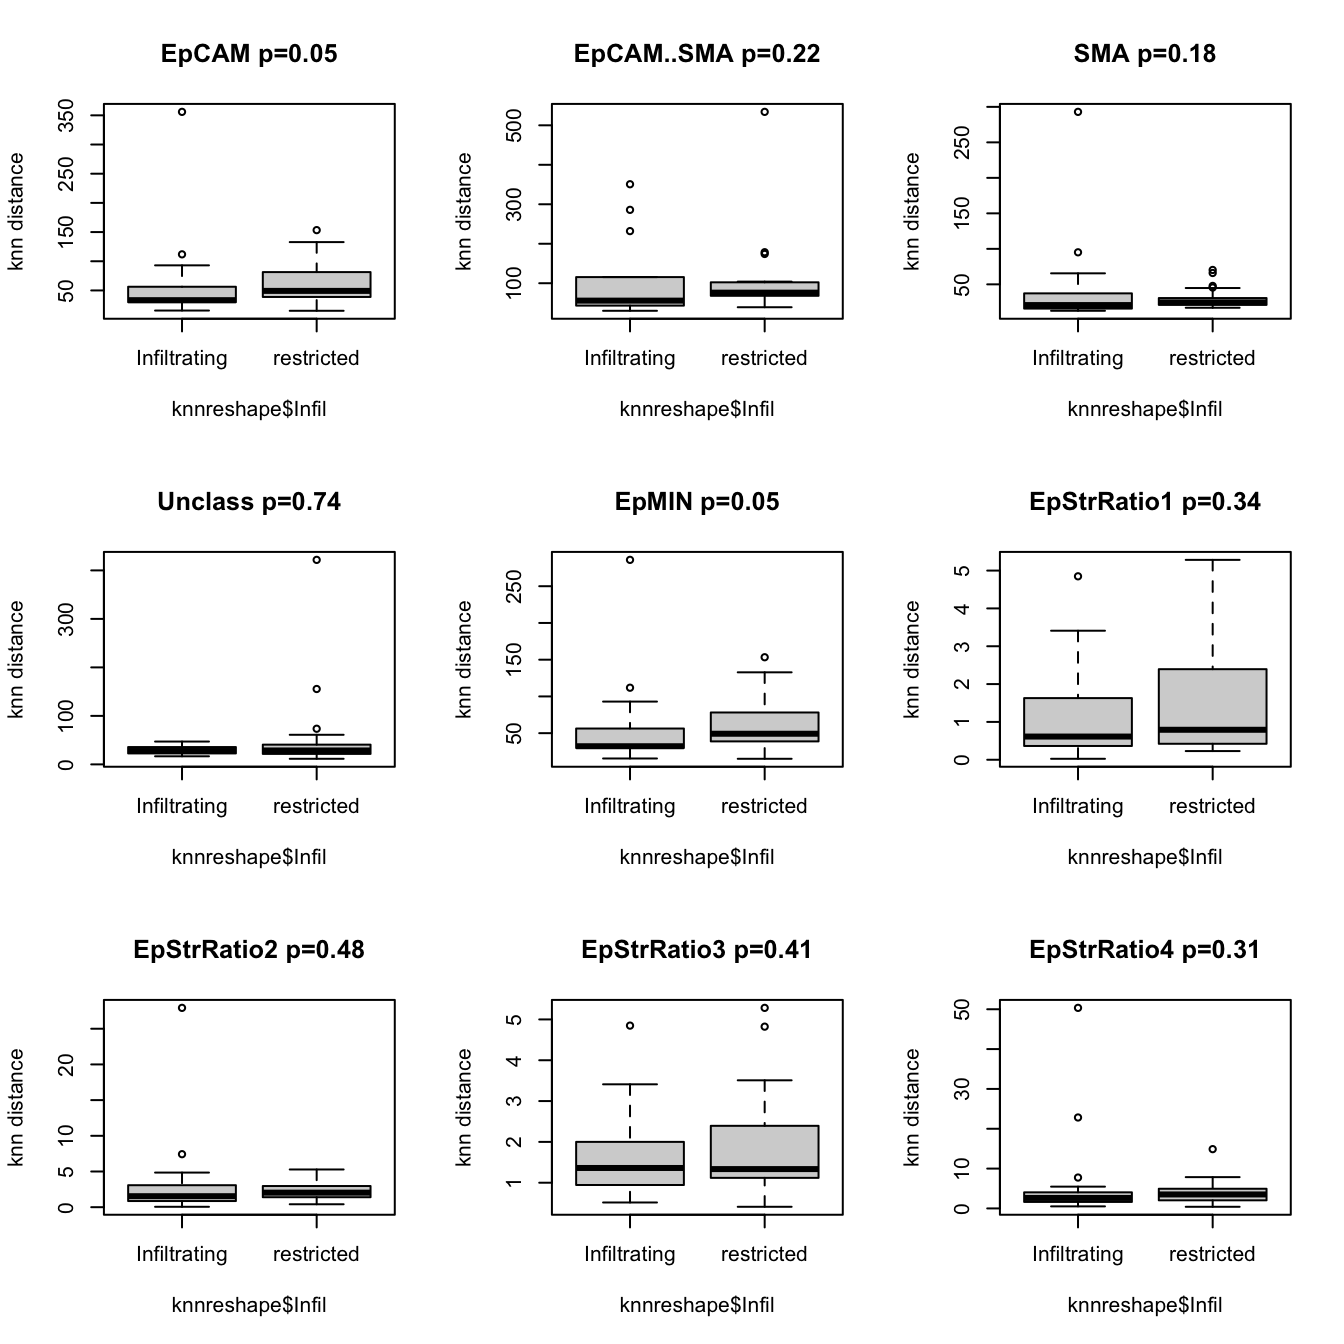
\includegraphics{RatDCIS-bookdown_files/figure-latex/unnamed-chunk-48-1.pdf} 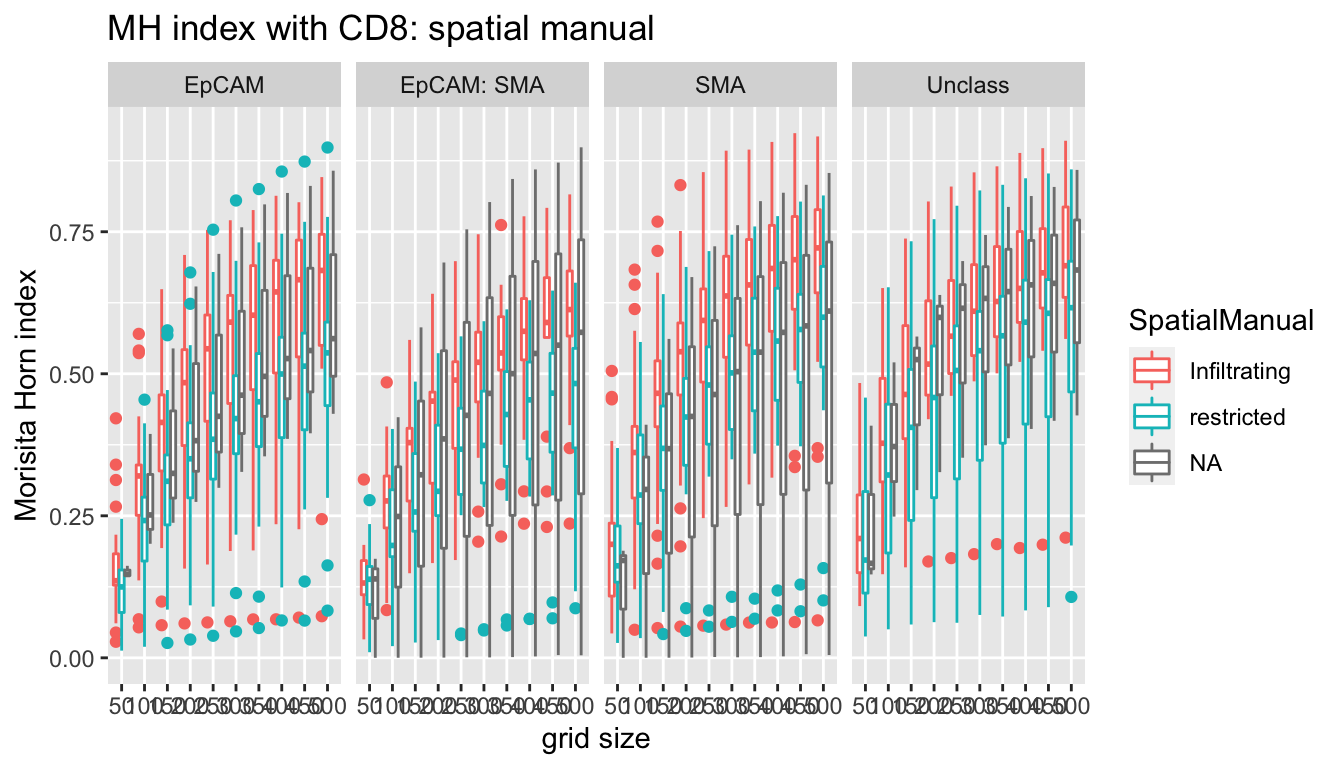
\includegraphics{RatDCIS-bookdown_files/figure-latex/unnamed-chunk-48-2.pdf} 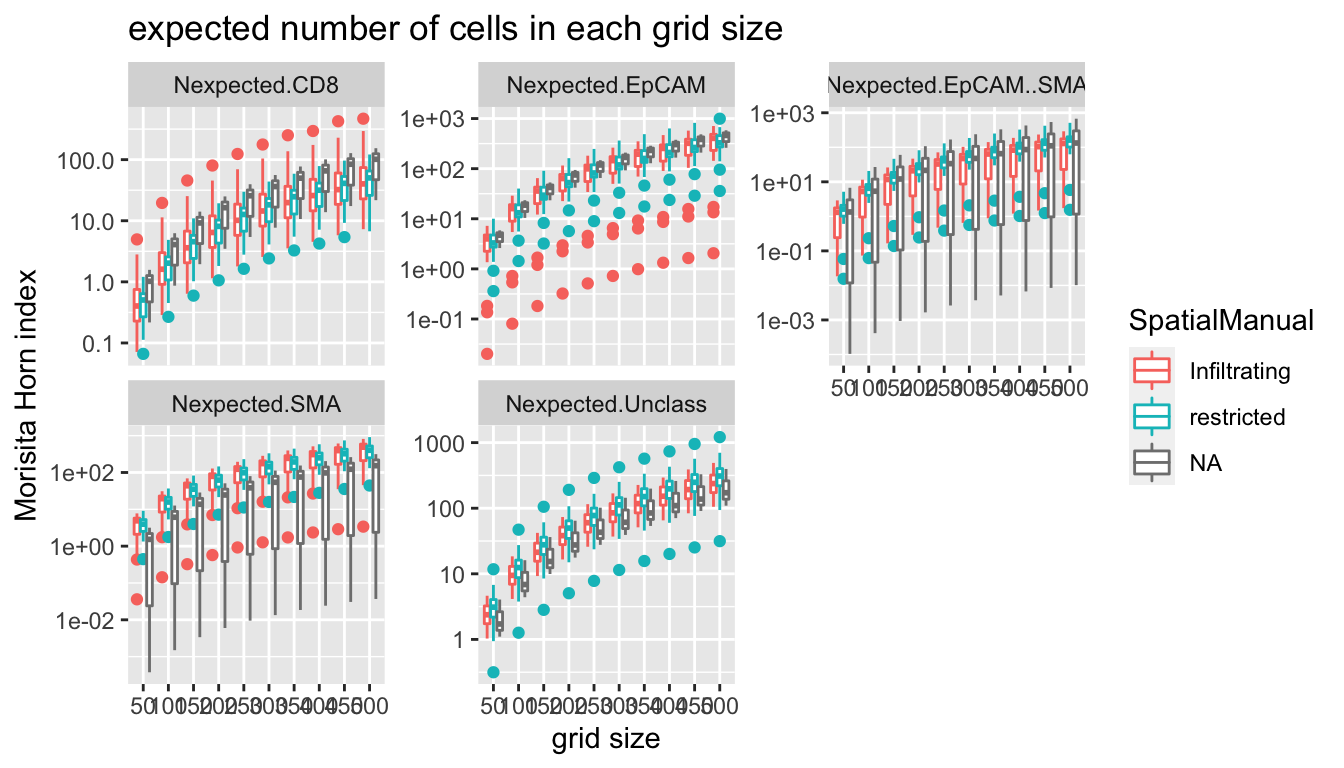
\includegraphics{RatDCIS-bookdown_files/figure-latex/unnamed-chunk-48-3.pdf}

With increasing grid size, optimal differences between infiltrating and restricted appear at the following sizes:

\begin{itemize}
\tightlist
\item
  epCAML 100um+
\item
  epcam:SMA most significant at 350+
\item
  SMA: 150+
\item
  Unclass:200+
\end{itemize}

We probably want to use a metric/gridsize of 250 um as the expected/mean number of cells in each grid is 10 here.
Other notes:

\begin{itemize}
\tightlist
\item
  double positive cells (EpCAM+SMA+) appear in predominantly the restricted cases?
\item
  higher SMA- stromal cells in restricted
\end{itemize}

Below, we check whether these metrics can differentiate between infiltrating and restricted tumors:

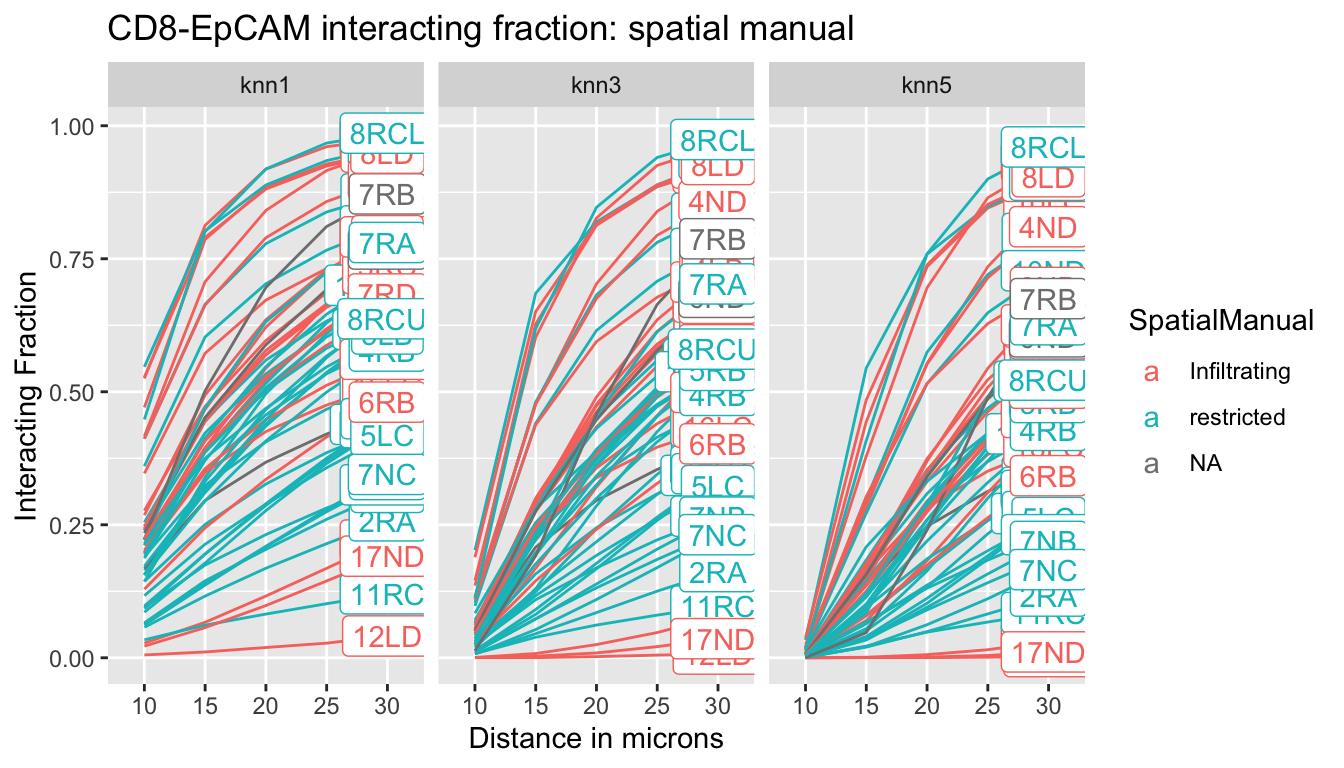
\includegraphics{RatDCIS-bookdown_files/figure-latex/unnamed-chunk-49-1.pdf}

The above analysis shows that the MH-index shows differences in mixing between CD8 cells and mixing with most cell types. However MH-CD8-to-Epcam to MH-CD8-to-stroma ratios do not support this difference.

\hypertarget{growth-2}{%
\subsection{Growth}\label{growth-2}}

Below are the MH indices with increasing grid-size for individual samples. In general, there is a subset of stable samples which have very high intermixing

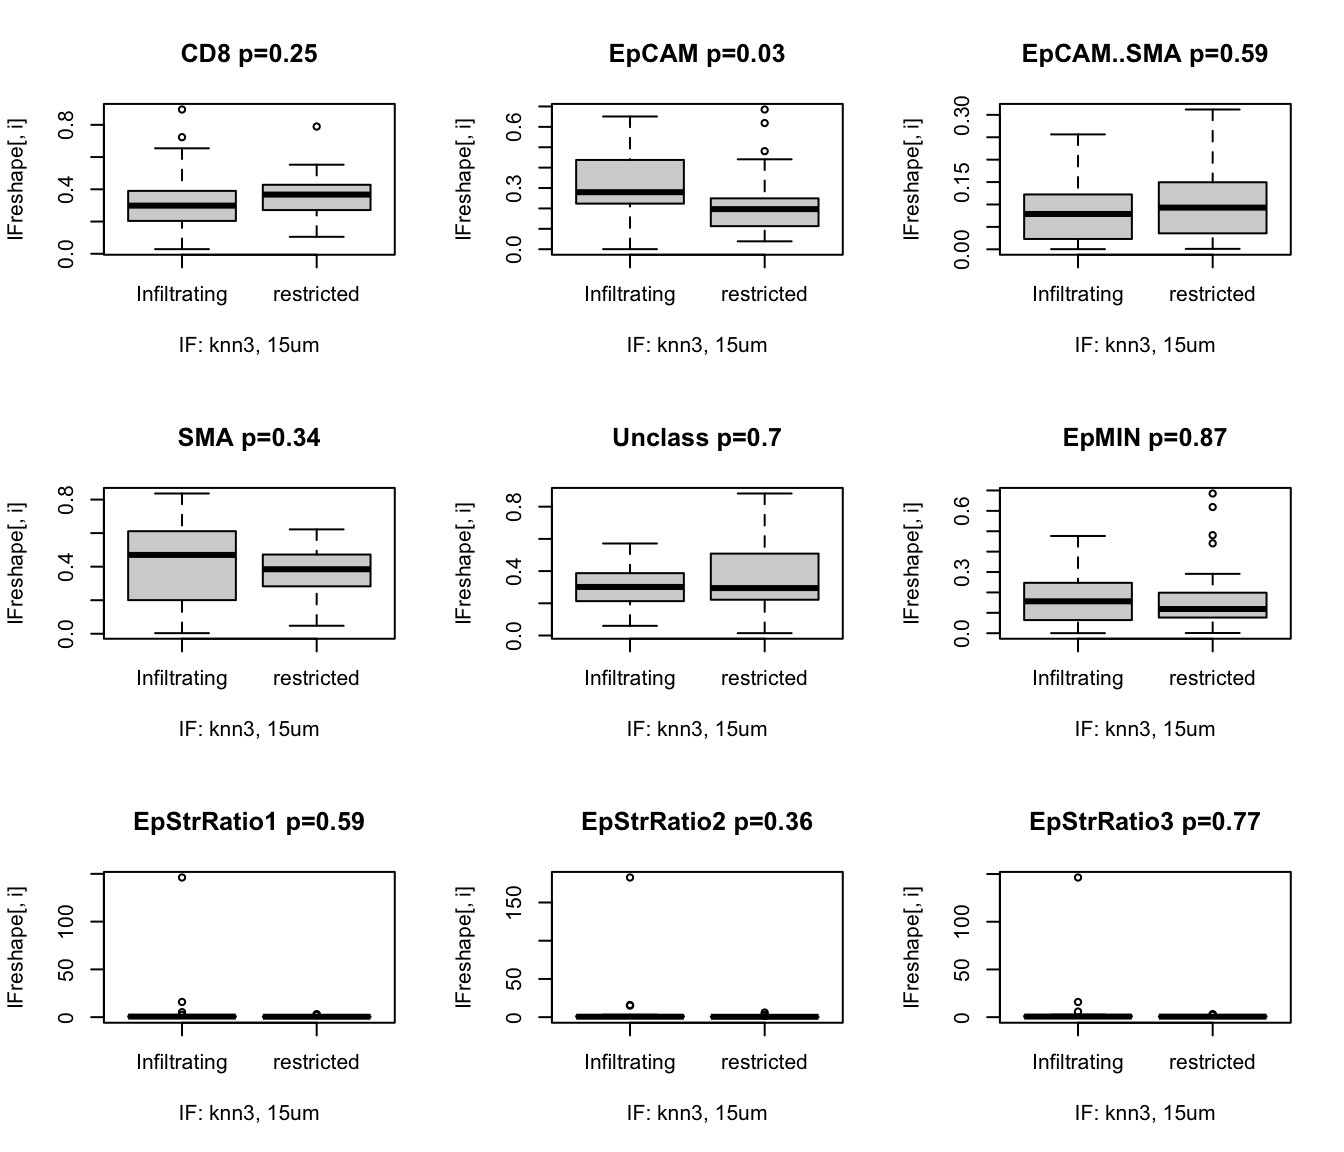
\includegraphics{RatDCIS-bookdown_files/figure-latex/unnamed-chunk-50-1.pdf} \includegraphics{RatDCIS-bookdown_files/figure-latex/unnamed-chunk-50-2.pdf}

Although the MH values for growing vs stable are not different, we can compare the mixing in epcam vs stroma in matched samples:

\includegraphics{RatDCIS-bookdown_files/figure-latex/unnamed-chunk-51-1.pdf}

\hypertarget{treatment-1}{%
\subsection{Treatment}\label{treatment-1}}

\includegraphics{RatDCIS-bookdown_files/figure-latex/unnamed-chunk-52-1.pdf} \includegraphics{RatDCIS-bookdown_files/figure-latex/unnamed-chunk-52-2.pdf}

There is no difference between the different spatial metrics compared to the vehicle, however, we can compare for a given treatment if there is a difference between the epcam and the stromal interaction scores. It appears that there is a difference only in the control, where SMA mixing is higher than EPcam mixing:

\includegraphics{RatDCIS-bookdown_files/figure-latex/unnamed-chunk-53-1.pdf}

\hypertarget{comparison-between-metrics}{%
\section{Comparison between metrics}\label{comparison-between-metrics}}

After assessing optimal parameters for each metric, in this section we assess which metric could be the best for spatial analysis.

Below is a table of the different metrics and their values for each sample

\begin{tabular}{l|r|r|r|l|l|l|r|r}
\hline
  & knn.EpCAM & IF.EpCAM & MH.EpCAM & Treatment & Growth & Infil & CD8frac & TumSize\\
\hline
10LB & 39.96193 & 0.2236555 & 0.4598790 & PDL1 & growing & Infiltrating & 0.0228977 & 35\\
\hline
10LC & 17.87345 & 0.4768745 & 0.5432610 & PDL1 & growing & Infiltrating & 0.0100341 & 25\\
\hline
10LD & 34.33110 & 0.2944373 & 0.6867357 & PDL1 & stable & Infiltrating & 0.0681088 & 10\\
\hline
10NA & 23.80977 & 0.4808547 & 0.4764461 & PDL1 & NA & restricted & 0.0465627 & 12\\
\hline
10ND & 26.20801 & 0.4408878 & 0.4181843 & PDL1 & stable & restricted & 0.0227195 & 15\\
\hline
10RBL & 44.92703 & 0.2213380 & 0.5857603 & PDL1 & growing & restricted & 0.0202715 & 40\\
\hline
10RBU & 87.12901 & 0.0816202 & 0.3840030 & PDL1 & NA & restricted & 0.0670641 & 12\\
\hline
11LB & 69.10296 & 0.2080105 & 0.2992537 & PDL1 & growing & NA & 0.1521777 & 25\\
\hline
11ND & 92.98237 & 0.0079816 & 0.5643066 & PDL1 & stable & Infiltrating & 0.3800672 & 3\\
\hline
11RC & 153.33513 & 0.0386688 & 0.0388372 & PDL1 & growing & restricted & 0.0504186 & 19\\
\hline
11RD & 73.82461 & 0.2323507 & 0.3847338 & PDL1 & growing & restricted & 0.0224452 & 25\\
\hline
12LD & 355.94915 & 0.0002809 & 0.1642608 & PDL1 & stable & Infiltrating & 0.0223693 & 6\\
\hline
13NA & 70.80101 & 0.1279338 & 0.3039013 & Vehicle & growing & restricted & 0.0355811 & 35\\
\hline
14NB & 49.22243 & 0.2540062 & 0.4353436 & PDL1+LY & growing & restricted & 0.1061520 & 23\\
\hline
14NC & 44.46686 & 0.1239597 & 0.3670808 & PDL1+LY & stable & restricted & 0.0541298 & 6\\
\hline
14RD & 31.50346 & 0.1681860 & 0.6214897 & PDL1+LY & stable & Infiltrating & 0.0103371 & 1\\
\hline
15LB & 32.69579 & 0.2226772 & 0.4642353 & PDL1+LY & growing & restricted & 0.0129612 & 10\\
\hline
15NC-D & 39.22818 & 0.1299775 & 0.4756601 & PDL1+LY & growing & restricted & 0.0107875 & 22\\
\hline
15ND & 15.54429 & 0.6025030 & 0.6063571 & PDL1+LY & stable & Infiltrating & 0.0104721 & 3\\
\hline
15RD & 91.07517 & 0.1578969 & 0.3729870 & PDL1+LY & growing & restricted & 0.0328312 & 17\\
\hline
16LA & 31.26867 & 0.2750368 & 0.3355138 & PDL1+LY & NA & Infiltrating & 0.0171528 & 5\\
\hline
16LC & 71.64542 & 0.2411490 & 0.0623470 & PDL1+LY & stable & Infiltrating & 0.0476926 & 7\\
\hline
16LD & 38.85862 & 0.3001624 & 0.5734648 & PDL1+LY & stable & Infiltrating & 0.0316168 & 24\\
\hline
16ND & 29.84045 & 0.2842939 & 0.5094333 & PDL1 & stable & Infiltrating & 0.0753308 & 25\\
\hline
16RD & 56.31604 & 0.2354937 & 0.3920871 & PDL1 & stable & Infiltrating & 0.0306486 & 3\\
\hline
17NA & 61.86642 & 0.0907525 & 0.3510232 & Vehicle & growing & restricted & 0.0472687 & 28\\
\hline
17ND & 111.85371 & 0.0029328 & 0.6112631 & Vehicle & stable & Infiltrating & 0.1115267 & 4\\
\hline
17RB & 16.70828 & 0.6275561 & 0.4630693 & Vehicle & growing & Infiltrating & 0.0411074 & 35\\
\hline
2N & 35.15413 & 0.2448721 & 0.3766073 & Vehicle & growing & restricted & 0.0301041 & 47\\
\hline
2RA & 132.80795 & 0.0452766 & 0.3252085 & Vehicle & growing & restricted & 0.0858192 & 20\\
\hline
2RD & 38.61221 & 0.1979009 & 0.6791816 & Vehicle & growing & restricted & 0.0742195 & 20\\
\hline
3LA & 46.09601 & 0.2865240 & 0.4162200 & Vehicle & growing & restricted & 0.0531246 & 12\\
\hline
3NB & 32.31159 & 0.4377911 & 0.7061056 & Vehicle & stable & Infiltrating & 0.2768299 & 6\\
\hline
3RB & 42.63162 & 0.2910751 & 0.4645950 & Vehicle & growing & restricted & 0.0266554 & 35\\
\hline
3RC & 32.11938 & 0.2962108 & 0.4965437 & Vehicle & growing & Infiltrating & 0.0232139 & 32\\
\hline
4LB & 30.99117 & 0.2903294 & 0.5447258 & Vehicle & growing & Infiltrating & 0.0244474 & 35\\
\hline
4NC & 15.33106 & 0.6851436 & 0.0901870 & Vehicle & growing & restricted & 0.0081388 & 15\\
\hline
4ND & 20.75556 & 0.4768080 & 0.5809047 & Vehicle & growing & Infiltrating & 0.0076245 & 20\\
\hline
4RB & 53.31478 & 0.1765476 & 0.3445324 & Vehicle & growing & restricted & 0.0280096 & 40\\
\hline
5LA & 41.12871 & 0.2471295 & 0.3724930 & Vehicle & stable & Infiltrating & 0.0453952 & 6\\
\hline
5LB & 41.91177 & 0.2807178 & 0.4690510 & Vehicle & growing & restricted & 0.0257830 & 4\\
\hline
5LC & 82.68448 & 0.1168545 & 0.1980203 & Vehicle & growing & restricted & 0.0515055 & 22\\
\hline
5LD & 91.41539 & 0.0735101 & 0.2028472 & Vehicle & stable & restricted & 0.0348108 & 15\\
\hline
5RB & 39.00602 & 0.1934315 & 0.4479302 & Vehicle & growing & restricted & 0.0596672 & 35\\
\hline
6LDU & 111.44785 & 0.1092889 & 0.2738092 & LY & growing & restricted & 0.0556253 & 32\\
\hline
6ND & 28.41556 & 0.2756628 & 0.4251078 & LY & growing & NA & 0.0815901 & 40\\
\hline
6RB & 76.37955 & 0.1446840 & 0.5947703 & LY & growing & Infiltrating & 0.1554804 & 18\\
\hline
6RC & 50.21453 & 0.1966022 & 0.5496400 & LY & growing & restricted & 0.0788010 & 40\\
\hline
7NB & 80.17580 & 0.0728176 & 0.1877309 & LY & growing & restricted & 0.0206734 & 31\\
\hline
7NC & 89.34399 & 0.0531233 & 0.2103338 & LY & growing & restricted & 0.0479457 & 40\\
\hline
7RA & 33.35958 & 0.2251296 & 0.4269972 & LY & stable & restricted & 0.0319310 & 8\\
\hline
7RB & 34.39737 & 0.1917334 & 0.7110689 & LY & growing & NA & 0.0169469 & 20\\
\hline
7RD & 44.13770 & 0.2386457 & 0.4019270 & LY & stable & Infiltrating & 0.0321690 & 20\\
\hline
8LD & 16.36623 & 0.6508906 & 0.7532812 & LY & stable & Infiltrating & 0.0562336 & 6\\
\hline
8RCL & 15.12966 & 0.6186366 & 0.7536385 & LY & growing & restricted & 0.0176691 & 12\\
\hline
8RCU & 50.00101 & 0.2347423 & 0.4676640 & LY & growing & restricted & 0.0287668 & 27\\
\hline
\end{tabular}

Firstly, we can compare the different metrics to determine how similar or different they are:

\includegraphics{RatDCIS-bookdown_files/figure-latex/unnamed-chunk-57-1.pdf}

Do any of these metrics associate with growth or treatments?

\includegraphics{RatDCIS-bookdown_files/figure-latex/unnamed-chunk-58-1.pdf}
We can also compare this to raw tumor size or growth rate data as well:

\includegraphics{RatDCIS-bookdown_files/figure-latex/unnamed-chunk-59-1.pdf}

\hypertarget{other-cell-types}{%
\section{Other cell types}\label{other-cell-types}}

We noted that the proportion of Unclassified cells seemed to be different between the treatments. Assess here whether the MH index for this cell type is associated with growth or treatment here:

\includegraphics{RatDCIS-bookdown_files/figure-latex/unnamed-chunk-62-1.pdf} \includegraphics{RatDCIS-bookdown_files/figure-latex/unnamed-chunk-62-2.pdf} \includegraphics{RatDCIS-bookdown_files/figure-latex/unnamed-chunk-62-3.pdf} \includegraphics{RatDCIS-bookdown_files/figure-latex/unnamed-chunk-62-4.pdf}

\hypertarget{expression-data}{%
\chapter{Expression data}\label{expression-data}}

This file looks at loading and pre-processing data for:

\begin{itemize}
\tightlist
\item
  differential gene expression analysis
\item
  PAM50 subtyping
\item
  uploading into CIBERSORT/TIMER
\end{itemize}

\hypertarget{running-alignment}{%
\section{Running alignment}\label{running-alignment}}

Samples were mapped in star using the following parameters. Note that the first two batches of samples run had shorter read lengths (\textasciitilde75 bp) whereas batch 3 had lengths of \textasciitilde150bp

\begin{Shaded}
\begin{Highlighting}[]
\CommentTok{## Not run here}
\NormalTok{STAR \textbackslash{}}
     \OperatorTok{--}\NormalTok{readFilesCommand zcat \textbackslash{}}
     \OperatorTok{--}\NormalTok{genomeDir }\OperatorTok{/}\NormalTok{n}\OperatorTok{/}\NormalTok{scratch2}\OperatorTok{/}\NormalTok{at268}\OperatorTok{/}\NormalTok{rn6_v2 \textbackslash{}}
     \OperatorTok{--}\NormalTok{sjdbGTFfile }\OperatorTok{/}\NormalTok{n}\OperatorTok{/}\NormalTok{scratch2}\OperatorTok{/}\NormalTok{at268}\OperatorTok{/}\NormalTok{rn6_v2}\OperatorTok{/}\NormalTok{rn6.refGene.gtf \textbackslash{}}
     \OperatorTok{--}\NormalTok{runThreadN }\DecValTok{10}\NormalTok{ \textbackslash{}}
     \OperatorTok{--}\NormalTok{runMode alignReads \textbackslash{}}
     \OperatorTok{--}\NormalTok{genomeLoad NoSharedMemory\textbackslash{}}
     \OperatorTok{--}\NormalTok{outSAMattributes NH HI AS nM NM\textbackslash{}}
     \OperatorTok{--}\NormalTok{outSAMstrandField intronMotif\textbackslash{}}
     \OperatorTok{--}\NormalTok{outFilterMultimapNmax }\DecValTok{20}\NormalTok{\textbackslash{}}
     \OperatorTok{--}\NormalTok{alignSJoverhangMin }\DecValTok{8}\NormalTok{\textbackslash{}}
     \OperatorTok{--}\NormalTok{readFilesIn }\OperatorTok{$}\DecValTok{1} \OperatorTok{$}\DecValTok{2}\NormalTok{ \textbackslash{}}
     \OperatorTok{--}\NormalTok{alignSJDBoverhangMin }\DecValTok{1}\NormalTok{\textbackslash{}}
     \OperatorTok{--}\NormalTok{outFilterMismatchNmax }\DecValTok{999}\NormalTok{\textbackslash{}}
     \OperatorTok{--}\NormalTok{outFilterMismatchNoverLmax }\FloatTok{0.1}\NormalTok{\textbackslash{}}
     \OperatorTok{--}\NormalTok{alignIntronMin }\DecValTok{20}\NormalTok{\textbackslash{}}
     \OperatorTok{--}\NormalTok{alignIntronMax }\DecValTok{1000000}\NormalTok{\textbackslash{}}
     \OperatorTok{--}\NormalTok{alignMatesGapMax }\DecValTok{1000000}\NormalTok{\textbackslash{}}
     \OperatorTok{--}\NormalTok{outFilterType BySJout\textbackslash{}}
     \OperatorTok{--}\NormalTok{outFilterScoreMinOverLread }\FloatTok{0.33}\NormalTok{ \textbackslash{}}
     \OperatorTok{--}\NormalTok{outFilterMatchNminOverLread }\FloatTok{0.33}\NormalTok{ \textbackslash{}}
     \OperatorTok{--}\NormalTok{limitSjdbInsertNsj }\DecValTok{1200000}\NormalTok{ \textbackslash{}}
     \OperatorTok{--}\NormalTok{outFilterIntronMotifs None \textbackslash{}}
     \OperatorTok{--}\NormalTok{alignSoftClipAtReferenceEnds Yes\textbackslash{}}
     \OperatorTok{--}\NormalTok{outSAMattrRGline ID}\OperatorTok{:}\ErrorTok{$}\DecValTok{4}\NormalTok{ SM}\OperatorTok{:}\ErrorTok{$}\DecValTok{4}\NormalTok{ \textbackslash{}}
     \OperatorTok{--}\NormalTok{chimSegmentMin }\DecValTok{15}\NormalTok{ \textbackslash{}}
     \OperatorTok{--}\NormalTok{chimJunctionOverhangMin }\DecValTok{15}\NormalTok{\textbackslash{}}
     \OperatorTok{--}\NormalTok{limitBAMsortRAM }\DecValTok{0}\NormalTok{\textbackslash{}}
     \OperatorTok{--}\NormalTok{outSAMtype BAM SortedByCoordinate\textbackslash{}}
     \OperatorTok{--}\NormalTok{outSAMunmapped Within \textbackslash{}}
     \OperatorTok{--}\NormalTok{quantMode GeneCounts transcriptomeSAM \textbackslash{}}
     \OperatorTok{--}\NormalTok{quantTranscriptomeBan IndelSoftclipSingleend \textbackslash{}}
     \OperatorTok{--}\NormalTok{outFileNamePrefix }\OperatorTok{$}\DecValTok{3}\NormalTok{ \textbackslash{}}
     \OperatorTok{--}\NormalTok{twopassMode Basic}
\end{Highlighting}
\end{Shaded}

In addition, RSEM was run to obtain TPM, rsem and FPKM counts.
Note: \href{http://hgdownload.soe.ucsc.edu/goldenPath/rn6/bigZips/genes/rn6.ncbiRefSeq.gtf.gz}{rn6.refGene.gtf.gz} was used to generate the RSEM library!(This is the may version)

\hypertarget{rna-initial-qc}{%
\section{RNA Initial QC}\label{rna-initial-qc}}

Default output from R showing the number of unique reads compared to multimapped, unmapped etc. This is shown for each batch.
Note that batch 3 has differences (high percentage of unmapped) compared to the other batches, possibly due to DNA contamination.

Below we check for three measures:

\begin{itemize}
\tightlist
\item
  mapped million reads (ideally, 10M+ reads)
\item
  Gene Sparsity: This is a measurement of the number of genes which have non-zero values. Ideally, would be greater than 10K, but values which are too high may also suggest contamination from DNA (unexpressed genes are also counted)
\item
  Varability: standard deviation of the transcriptomic counts. If this value is too low, would suggest that high DNA contamination, non-representative transcriptome.
\end{itemize}

\includegraphics{RatDCIS-bookdown_files/figure-latex/unnamed-chunk-66-1.pdf} \includegraphics{RatDCIS-bookdown_files/figure-latex/unnamed-chunk-66-2.pdf} \includegraphics{RatDCIS-bookdown_files/figure-latex/unnamed-chunk-66-3.pdf}

Samples to remove from analysis:

The thresholds indicated below are based on the above density plots, and removes cases which are \textless1.5 SD of the mean

\begin{itemize}
\tightlist
\item
  low total number of mapped reads (under 1.5M)
\item
  sparsity: less than 8K genes
\item
  variability : threshold under 500
\end{itemize}

The omitted samples are:

\begin{tabular}{l|r|r|r|r|l|l}
\hline
  & MappedReadsM & GeneSparsityK & Batch & GeneVariabilityCounts & Type & names\\
\hline
6R\_C\_CD45 & 2.287110 & 5.585 & 2 & 1063.38925 & CD45 & 6R\_C\_CD45\\
\hline
10L\_B\_DN & 0.864838 & 3.308 & 2 & 559.30659 & DN & 10L\_B\_DN\\
\hline
NMU1\_LL\_Ep & 1.032440 & 16.708 & 3 & 69.82645 & Ep & NMU1\_LL\_Ep\\
\hline
NMU5\_LA\_Ep & 0.500429 & 15.707 & 3 & 35.56084 & Ep & NMU5\_LA\_Ep\\
\hline
Control1\_\_Ep & 8.224593 & 5.800 & 1 & 3164.00515 & Ep & Control1\_\_Ep\\
\hline
NMU13\_RAU\_Ep & 3.049733 & 7.242 & 1 & 1069.99912 & Ep & NMU13\_RAU\_Ep\\
\hline
\end{tabular}

We are left with 110 samples.

There are 47, 32, 31 samples in the CD45, Ep, DN fractions.

There are 20, 49, 41 samples from batches 1, 2 and 3 respectively.

\hypertarget{normalisation}{%
\section{Normalisation}\label{normalisation}}

Run through DESEq and normalise the library. Using all samples, we run the model:

expression \textasciitilde{} Celltype + factor (Batch)

and keep the genes which have a total count of at least half the number of samples. ie.
\$ sum(gene\_i) \textgreater{} N\_\{samples\}/2 \$

\hypertarget{preliminary-visualisation-to-remove-outliers}{%
\subsection{preliminary visualisation (to remove outliers)}\label{preliminary-visualisation-to-remove-outliers}}

Below are PCA plots based on:

\begin{itemize}
\tightlist
\item
  Batch
\item
  CellType
\end{itemize}

\includegraphics{RatDCIS-bookdown_files/figure-latex/vsd-transform-1.pdf} \includegraphics{RatDCIS-bookdown_files/figure-latex/vsd-transform-2.pdf} \includegraphics{RatDCIS-bookdown_files/figure-latex/vsd-transform-3.pdf}

Batches in general separate out well, however, some samples appear to be outliers in comparison to the main group. We look in closer detail the CD45, DN and EpCAM populations.

In the CD45 population, narrow down to only immune related genes to see if there is a difference.

\includegraphics{RatDCIS-bookdown_files/figure-latex/unnamed-chunk-69-1.pdf} \includegraphics{RatDCIS-bookdown_files/figure-latex/unnamed-chunk-69-2.pdf} \includegraphics{RatDCIS-bookdown_files/figure-latex/unnamed-chunk-69-3.pdf}

Based on the above plots, we remove the following outliers and re-run the normalisation:

\begin{itemize}
\tightlist
\item
  2R\_D\_DN
\item
  4L\_B\_CD45
\end{itemize}

\hypertarget{processing-files-for-external-software}{%
\section{Processing files for external software}\label{processing-files-for-external-software}}

We also process these files for external software:

\begin{longtable}[]{@{}ll@{}}
\toprule
Software & RNA-data\tabularnewline
\midrule
\endhead
PAM50 & rsem data after quantile normalised, genes converted to human\tabularnewline
TIMER & TPM values, retain rat ids\tabularnewline
xcell & rsem data, genes converted ti human\tabularnewline
cibersort & tpm?? convert to rat genes and use lm22 rat\tabularnewline
\bottomrule
\end{longtable}

\begin{verbatim}
## named integer(0)
\end{verbatim}

\begin{verbatim}
## named integer(0)
\end{verbatim}

Save the mouse names for TIMER cistrome: check that this is actually required for TIMER

\hypertarget{rna-data-preliminary-plots}{%
\chapter{RNA data: preliminary plots}\label{rna-data-preliminary-plots}}

Prior to doing any comparative analysis, we will look at the following plots to get an overview of the data.

\hypertarget{pca-plots}{%
\section{PCA plots}\label{pca-plots}}

We can check the new PCA plots, and overlay parameters of interest including treatment, growth, tumor size, CD8 fraction, spatial distribution.

\includegraphics{RatDCIS-bookdown_files/figure-latex/vsd-corrected-1.pdf} \includegraphics{RatDCIS-bookdown_files/figure-latex/vsd-corrected-2.pdf} \includegraphics{RatDCIS-bookdown_files/figure-latex/vsd-corrected-3.pdf} \includegraphics{RatDCIS-bookdown_files/figure-latex/vsd-corrected-4.pdf} \includegraphics{RatDCIS-bookdown_files/figure-latex/vsd-corrected-5.pdf} \includegraphics{RatDCIS-bookdown_files/figure-latex/vsd-corrected-6.pdf} \includegraphics{RatDCIS-bookdown_files/figure-latex/vsd-corrected-7.pdf} \includegraphics{RatDCIS-bookdown_files/figure-latex/vsd-corrected-8.pdf}

In addition, we can look at the CD45 population and the distributions based on CD8 content and spatial infiltration

\includegraphics{RatDCIS-bookdown_files/figure-latex/unnamed-chunk-73-1.pdf} \includegraphics{RatDCIS-bookdown_files/figure-latex/unnamed-chunk-73-2.pdf} \includegraphics{RatDCIS-bookdown_files/figure-latex/unnamed-chunk-73-3.pdf} \includegraphics{RatDCIS-bookdown_files/figure-latex/unnamed-chunk-73-4.pdf}

\hypertarget{expression-patterns-by-cell-type}{%
\section{Expression patterns by cell type}\label{expression-patterns-by-cell-type}}

Below, we check whether the different fractions are expressing expected markers

The cell types are:

\begin{itemize}
\tightlist
\item
  Red: Cd45
\item
  Epcam: green
\item
  DN:blue
\end{itemize}

Reference Genes:

\begin{itemize}
\tightlist
\item
  purple: immune
\item
  blue: epithelial
\item
  green: stroma
\item
  orange: myoepithelial
\item
  red: endothelial
\end{itemize}

Below, we see that the CD45 cells separate from the Ep/DN populations have high expression of immune related genes including CD3, CD4, IFNG.

However, the DN/Ep fractions are more intermixed. The DN fraction has expression of keratins, as well as fibroblast markers (Acta1), and myeoepithelial markers (Tp63)

\includegraphics{RatDCIS-bookdown_files/figure-latex/unnamed-chunk-74-1.pdf} \includegraphics{RatDCIS-bookdown_files/figure-latex/unnamed-chunk-74-2.pdf}

\hypertarget{deseq-analysis}{%
\chapter{DESeq analysis}\label{deseq-analysis}}

This document sets up DESeq runs to compare:

\begin{itemize}
\tightlist
\item
  DN vs Ep samples
\item
  growing vs stable samples (all 3 fractions)
\item
  treatments (all 3 fractions)
\item
  spatial patterns (all 3 fractions)
\end{itemize}

The outputs of these analyses will be used for Gene Set Enrichment Analysis,
using MSigDB databases (c2, c5, hallmark), alongside pathways from Metacore (Process Networks, Pathway Maps)

\hypertarget{dn-vs-ep}{%
\section{DN vs Ep}\label{dn-vs-ep}}

What is the difference between DN and Ep fractions?
Select for genes with p value cut off of 0.05 and log2 fold change of 1.5.
Also, when visualising top genes, select for base expression greater than 100

\begin{verbatim}
## 
## out of 15301 with nonzero total read count
## adjusted p-value < 0.1
## LFC > 0 (up)       : 2172, 14%
## LFC < 0 (down)     : 1188, 7.8%
## outliers [1]       : 463, 3%
## low counts [2]     : 779, 5.1%
## (mean count < 2)
## [1] see 'cooksCutoff' argument of ?results
## [2] see 'independentFiltering' argument of ?results
\end{verbatim}

\begin{tabular}{l|r|r|r|r|r|r}
\hline
  & baseMean & log2FoldChange & lfcSE & stat & pvalue & padj\\
\hline
Fap & 147.505781 & 3.791943 & 0.6564706 & 5.776257 & 0.0000000 & 0.0000009\\
\hline
Vim & 13706.172521 & 1.832658 & 0.3361022 & 5.452680 & 0.0000000 & 0.0000035\\
\hline
RGD1565355 & 4.841686 & -2.427252 & 0.8547683 & -2.839661 & 0.0045162 & 0.0307470\\
\hline
Mme & 214.622521 & 2.418161 & 0.5763311 & 4.195784 & 0.0000272 & 0.0005517\\
\hline
Cnn1 & 618.403495 & 1.572872 & 0.4698537 & 3.347578 & 0.0008152 & 0.0081399\\
\hline
Tp63 & 145.596811 & 2.047668 & 0.4768123 & 4.294494 & 0.0000175 & 0.0003907\\
\hline
Cdh5 & 114.363936 & 1.899697 & 0.6674752 & 2.846093 & 0.0044259 & 0.0302941\\
\hline
Itgam & 289.807818 & -2.251148 & 0.5564127 & -4.045824 & 0.0000521 & 0.0009532\\
\hline
Col1a1 & 35939.383628 & 4.962384 & 0.7227443 & 6.866031 & 0.0000000 & 0.0000000\\
\hline
Krt14 & 949.200864 & 1.834436 & 0.4774425 & 3.842214 & 0.0001219 & 0.0018837\\
\hline
Acta2 & 489.516373 & 1.678424 & 0.4013367 & 4.182086 & 0.0000289 & 0.0005810\\
\hline
Cd38 & 370.418350 & 1.897076 & 0.4719555 & 4.019608 & 0.0000583 & 0.0010370\\
\hline
Cdh3 & 100.102955 & 1.705776 & 0.4293903 & 3.972553 & 0.0000711 & 0.0012132\\
\hline
\end{tabular}

\includegraphics{RatDCIS-bookdown_files/figure-latex/ep-v-dn-1.pdf} \includegraphics{RatDCIS-bookdown_files/figure-latex/ep-v-dn-2.pdf} \includegraphics{RatDCIS-bookdown_files/figure-latex/ep-v-dn-3.pdf} \includegraphics{RatDCIS-bookdown_files/figure-latex/ep-v-dn-4.pdf}

Note that there seems to be two main groups of Ep cells:

The first one is enriched for canonical tumour progression pathways: eg. expression of wnt, fox1a etc.
The second one doesn't seem to have as high expression of these genes, but have high immune related signalling pathways

\hypertarget{set-up-the-comparisons}{%
\section{Set-up the comparisons}\label{set-up-the-comparisons}}

Separate out the tables into CD45, DN and Ep fractions. Compare

\begin{enumerate}
\def\labelenumi{\arabic{enumi}.}
\tightlist
\item
  Differences based on treatment (and treatment vs control)
\item
  Specific treatments vs control
\item
  Growing vs stable (overall)
\item
  Growing vs stable (in each subgroup)
\end{enumerate}

Check there are enough samples in each subgroup:

\begin{verbatim}
## [1] "number of samples for each treatment and growth rate"
\end{verbatim}

\begin{verbatim}
## , ,  = growing
## 
##       
##        LY PDL1 PDL1+LY Vehicle
##   CD45  5    5       5      11
##   DN    3    5       4       9
##   Ep    3    4       2       2
## 
## , ,  = stable
## 
##       
##        LY PDL1 PDL1+LY Vehicle
##   CD45  2    2       3       1
##   DN    1    2       4       2
##   Ep    1    3       3       2
\end{verbatim}

\includegraphics{RatDCIS-bookdown_files/figure-latex/unnamed-chunk-75-1.pdf} \includegraphics{RatDCIS-bookdown_files/figure-latex/unnamed-chunk-75-2.pdf}

Setup the following comparisons for each cell type:

expression \textasciitilde{} growing + treatment + batch (exclude 1) (start with vehicle vs some treatment)

4 categories only: immunotherapy vs non-immuno

Separate out the tables into CD45, DN and Ep fractions. Compare:

\begin{enumerate}
\def\labelenumi{\arabic{enumi}.}
\tightlist
\item
  Treatment (EpddsTreat)
\item
  Comp4: Growth + any immunotherapy treatment (Epdds)
\item
  Comp8: Growth + immunotherapy (EpddsTreatG)
\item
  Growth alone: (EpddsGrowth)
\item
  MH index: (EpddsStrMH)
\item
  Interacting Fraction (EpddsStrIF)
\item
  knn values (EpddsStrknn)
\item
  CD8 content (EpddsCD8)
\item
  Manual scoring spatial (EpddsSpatMan)
\item
  MH index + CD8 frac (Epddscd8MH)
\end{enumerate}

We remove genes which have 0 counts in more than half the samples, and genes which have a row sum less than 10\^{}(log10(mean(rowsums))-log10(sd(rowsums)))

\includegraphics{RatDCIS-bookdown_files/figure-latex/deseq-assoc-runs-1.pdf}

temp insertion: do comparison of differences in spatial with outcome:

\hypertarget{pca-plots-1}{%
\section{PCA plots}\label{pca-plots-1}}

check whether these are needed?

Also check the variance with the different samples

\includegraphics{RatDCIS-bookdown_files/figure-latex/unnamed-chunk-76-1.pdf} \includegraphics{RatDCIS-bookdown_files/figure-latex/unnamed-chunk-76-2.pdf} \includegraphics{RatDCIS-bookdown_files/figure-latex/unnamed-chunk-76-3.pdf} \includegraphics{RatDCIS-bookdown_files/figure-latex/unnamed-chunk-76-4.pdf} \includegraphics{RatDCIS-bookdown_files/figure-latex/unnamed-chunk-76-5.pdf} \includegraphics{RatDCIS-bookdown_files/figure-latex/unnamed-chunk-76-6.pdf} \includegraphics{RatDCIS-bookdown_files/figure-latex/unnamed-chunk-76-7.pdf} \includegraphics{RatDCIS-bookdown_files/figure-latex/unnamed-chunk-76-8.pdf} \includegraphics{RatDCIS-bookdown_files/figure-latex/unnamed-chunk-76-9.pdf} \includegraphics{RatDCIS-bookdown_files/figure-latex/unnamed-chunk-76-10.pdf} \includegraphics{RatDCIS-bookdown_files/figure-latex/unnamed-chunk-76-11.pdf} \includegraphics{RatDCIS-bookdown_files/figure-latex/unnamed-chunk-76-12.pdf} \includegraphics{RatDCIS-bookdown_files/figure-latex/unnamed-chunk-76-13.pdf} \includegraphics{RatDCIS-bookdown_files/figure-latex/unnamed-chunk-76-14.pdf} \includegraphics{RatDCIS-bookdown_files/figure-latex/unnamed-chunk-76-15.pdf} \includegraphics{RatDCIS-bookdown_files/figure-latex/unnamed-chunk-76-16.pdf} \includegraphics{RatDCIS-bookdown_files/figure-latex/unnamed-chunk-76-17.pdf} \includegraphics{RatDCIS-bookdown_files/figure-latex/unnamed-chunk-76-18.pdf}

\hypertarget{results-differences-in-the-epithelial-fraction}{%
\subsection{Results : differences in the epithelial fraction}\label{results-differences-in-the-epithelial-fraction}}

Save to file the differences in the epithelial fractions

\begin{verbatim}
## 
## growingcontrol     growingimm  stablecontrol      stableimm 
##              2              9              2              7
\end{verbatim}

\hypertarget{gsea}{%
\section{GSEA}\label{gsea}}

\begin{itemize}
\tightlist
\item
  may need to convert gene names into HUGO symbols
\end{itemize}

Prepare for GSEA: This takes approximately 15 minutes

\hypertarget{cd45-comparisons}{%
\section{CD45 comparisons}\label{cd45-comparisons}}

\hypertarget{dn-comparisons}{%
\section{DN comparisons}\label{dn-comparisons}}

\includegraphics{RatDCIS-bookdown_files/figure-latex/dn-samples-gsea-1.pdf}

\hypertarget{deseq-analysis-1}{%
\chapter{DESeq analysis}\label{deseq-analysis-1}}

\hypertarget{summary-plots}{%
\subsection{Summary plots}\label{summary-plots}}

Quick plot of the differences in number of differential genes:

\begin{verbatim}
##   Frac  dir                        variable value
## 1   Ep down stablecontrol_vs_growingcontrol     1
## 2   Ep   up stablecontrol_vs_growingcontrol     1
## 3   CD down stablecontrol_vs_growingcontrol   830
## 4   CD   up stablecontrol_vs_growingcontrol   524
## 5   DN down stablecontrol_vs_growingcontrol   152
## 6   DN   up stablecontrol_vs_growingcontrol    22
\end{verbatim}

\includegraphics{RatDCIS-bookdown_files/figure-latex/unnamed-chunk-81-1.pdf}

\begin{verbatim}
##   Frac  dir                        variable value
## 1 <NA> <NA> stablecontrol_vs_growingcontrol     2
## 2 <NA> <NA> stablecontrol_vs_growingcontrol     2
## 3 <NA> <NA> stablecontrol_vs_growingcontrol     1
## 4 <NA> <NA> stablecontrol_vs_growingcontrol    11
## 5 <NA> <NA> stablecontrol_vs_growingcontrol     2
## 6 <NA> <NA> stablecontrol_vs_growingcontrol     9
\end{verbatim}

Any commonly changed genes in any of the lists?
Plot lists:
* Pearson correlation of all the samples
* Unlist all, and pick out genes which are impacted in at least 1 comparison

CD45 comparisons

DN samples:

\hypertarget{focus-mainly-on-growing-vs-stable}{%
\section{Focus mainly on growing vs stable:}\label{focus-mainly-on-growing-vs-stable}}

Check: Is the difference between stable and growing just MHC expression?

\hypertarget{comapre-dn-samples-pam50-lum-vs-basalnormal}{%
\subsection{comapre DN samples: PAM50 Lum vs Basal/Normal?}\label{comapre-dn-samples-pam50-lum-vs-basalnormal}}

  \bibliography{book.bib,packages.bib}

\end{document}
